% =====================================================================
%  Accelerating the Flux MMDiT on PLENA  (benchmarked on Open-Sora)
%  BEng final report — Imperial College London, EEE
%  Author: Ziqian Gao
%
%  Self-contained: compile with lualatex (no external .cls needed).
% =====================================================================
\documentclass[11pt]{report}

\usepackage{fontspec}
\usepackage[a4paper,margin=2.5cm]{geometry}
\usepackage{graphicx}
\usepackage{amsmath}
\usepackage{amssymb}
\usepackage{booktabs}
\usepackage{longtable}
\usepackage{array}
\usepackage{xcolor}
\usepackage{setspace}
\usepackage[hidelinks]{hyperref}
\usepackage{titlesec}
\usepackage{caption}
\usepackage[ruled,linesnumbered]{algorithm2e}
\usepackage{multirow}
\usepackage{tikz}
\usetikzlibrary{positioning,arrows.meta,fit,backgrounds,calc,decorations.pathreplacing}

\setstretch{1.15}
\graphicspath{{./}{transactional_emulator/testbench/}}

\begin{document}

% ---------------------------------------------------------------------
% TITLE PAGE
% ---------------------------------------------------------------------
\begin{titlepage}
\centering
\vspace*{1cm}

\includegraphics[height=1.6cm]{IC_New_Logo.pdf}\\[1.2cm]

{\large Imperial College London\par}
{\normalsize Department of Electrical and Electronic Engineering\par}

\vspace{2.5cm}

{\large BEng Final Year Project Report\par}
\vspace{0.4cm}
{\large Electrical and Electronic Engineering\par}

\vspace{2.5cm}

{\LARGE\bfseries Accelerating the Flux MMDiT on PLENA\par}
\vspace{0.5cm}
{\Large Benchmarked on Open-Sora\par}

\vspace{2.5cm}

{\large\bfseries Ziqian Gao\par}
\vspace{0.3cm}
{\normalsize Supervisor: Dr N.S.\ Surname\par}

\vfill

{\normalsize 2026\par}
\end{titlepage}

% ---------------------------------------------------------------------
% ABSTRACT
% ---------------------------------------------------------------------
\chapter*{Abstract}
\addcontentsline{toc}{chapter}{Abstract}

The multimodal diffusion transformer (MMDiT), introduced by Flux, has
become one of the most widely adopted backbones in modern generative AI.
It powers text-to-image and text-to-video diffusion models such as
Open-Sora, and the same structure is reused well beyond generation: large
multimodal models such as Qwen and a growing number of robotics
vision-language-action (VLA) models build on the MMDiT. It is therefore a
remarkably general and capable structure --- but also an extremely
expensive one to serve. One MMDiT pass costs about the same as a single
\emph{prefill} forward of a comparably sized language model, but producing
one output runs the backbone on the order of \textbf{150 times} (tens of
denoising steps, each evaluated on three classifier-free-guidance branches),
where the language model runs a single prefill pass per prompt. A diffusion
generation therefore pays a fixed ${\sim}150$-pass tax that a language model
does not, which is precisely why systems of this class are so costly to serve
and why the per-pass efficiency of the backbone is what matters.

This report accelerates the \textbf{Flux MMDiT} on \textbf{PLENA}, a
systolic-array accelerator, and uses \textbf{Open-Sora} --- a real model
built on the same MMDiT --- as the benchmark, running it at its true
dimensions and weights. The MMDiT is built from two block types, a
double-stream block (DSB) and a single-stream block (SSB), which together
account for essentially all of the compute; both are implemented and
analysed across the full model lifecycle: low-precision inference
(MX-E4M3 / FP8) and high-precision training (the backward pass and the
optimiser step).

The work is evaluated along three axes --- \textbf{accuracy},
\textbf{latency}, and \textbf{power}. On accuracy, the whole MMDiT runs in
FP8 at a cosine of \textbf{0.9994} against the FP32 reference with no
fine-tuning, and the error neither accumulates with depth nor over the
denoising loop. On latency and energy, a PLENA deployment matched to one
NVIDIA A100's compute budget on the same 7\,nm node reaches
\textbf{$\sim$0.8$\times$} of the A100's wall-clock at roughly
\textbf{one third} of its energy per generation. The same analysis carries
into training. Bringing both the time and the energy of this
high-demand structure down to about a third of the GPU baseline is a
result that transfers well beyond video generation, to every model that
shares the MMDiT backbone.

% ---------------------------------------------------------------------
% ORIGINALITY STATEMENT  (front matter — to fill later)
% ---------------------------------------------------------------------
\chapter*{Statement of Originality}
\addcontentsline{toc}{chapter}{Statement of Originality}

% [TO WRITE] Declaration that the work is the author's own, with all
% sources properly cited.

% ---------------------------------------------------------------------
% ACKNOWLEDGEMENTS  (front matter — to fill later)
% ---------------------------------------------------------------------
\chapter*{Acknowledgements}
\addcontentsline{toc}{chapter}{Acknowledgements}

% [TO WRITE] Thanks to supervisor, group, family, etc.

% ---------------------------------------------------------------------
% TABLE OF CONTENTS / LIST OF FIGURES / LIST OF ACRONYMS
% ---------------------------------------------------------------------
\tableofcontents

\listoffigures
\addcontentsline{toc}{chapter}{List of Figures}

% --- List of Acronyms (placeholder — to fill later) ---
\chapter*{List of Acronyms}
\addcontentsline{toc}{chapter}{List of Acronyms}

% [TO WRITE] e.g. MMDiT, DSB, SSB, DiT, VLA, ISA, HBM, SRAM, MAC,
% FP8, MX-E4M3, RoPE, QAT, PTQ, ...


% #####################################################################
% CHAPTER 1 — INTRODUCTION
% #####################################################################
\chapter{Introduction}
\label{ch:intro}

\section{Motivation}
\label{sec:motivation}

Generative diffusion models have become the dominant approach to
high-quality image and video synthesis, but they are extraordinarily
expensive to run. The reason is not that any single network evaluation is
unusually large --- one forward pass through the diffusion backbone is
comparable in cost to a single \emph{prefill} forward of a similarly sized
language model, both being one dense pass over the whole token sequence. The
reason is \emph{how many times} that pass must be repeated to produce a
single output.

It is worth being precise about this, because it is easy to misread. The
right point of comparison is an LLM's \emph{prefill} --- the one full,
dense forward it runs over the entire prompt. A text-to-image or
text-to-video prompt costs the diffusion model roughly that same prefill-cost
\emph{per denoising step}, and a generation runs \emph{tens} of such steps,
because turning noise into an output is an iterative refinement loop with no
cache and no reuse between steps: \textbf{every step re-evaluates the entire
backbone over the entire token sequence from scratch}. On top of that, each
step does not evaluate the backbone once but \emph{three} times, once for
each branch of classifier-free guidance (Section~\ref{sec:diffusion}),
batched into one forward. So where an LLM does a single prefill-class pass
per prompt, a diffusion generation does
\[
\underbrace{S}_{\text{denoising steps}} \times
\underbrace{3}_{\text{CFG branches}}
\;\approx\; 50 \times 3 \;=\; \mathbf{150}
\]
of them. \textbf{The $150\times$ is a multiplier on the \emph{number of
prefill-class passes}, not on the size of any single pass.} For modern
text-to-video systems this backbone is the \textbf{multimodal diffusion
transformer (MMDiT)}, so a generation drives a large, dense network
${\sim}150$ times over, and it is this repetition --- not any one evaluation
--- that produces the very large wall-clock and energy figures that make
video generation so costly to serve at scale. It also means the lever that
matters is the \emph{per-pass} efficiency of the backbone: shave one pass and
you shave it $150$ times.

The difficulty of the MMDiT is of a different kind from an LLM's. Its
structure is extremely regular --- a fixed stack of identical transformer
blocks over a fixed-length token sequence --- so it never runs into the
autoregressive-decode and key/value-cache problems that dominate LLM
serving. What it has instead is sheer arithmetic volume: dense
general-matrix-multiplies (GEMMs) and full bidirectional attention over a
long joint sequence, executed the same way every pass. This regularity
makes the MMDiT an ideal target for a dedicated matrix accelerator, where
a systolic array can be kept near full utilisation, but the raw cost
makes any efficiency gain valuable.

What makes the effort worthwhile is that the MMDiT is not a niche
structure. It was introduced by \textbf{Flux}~\cite{bfl2024flux} ---
itself building on the MMDiT design of Stable Diffusion~3~\cite{esser2024sd3}
and the diffusion-transformer (DiT)~\cite{peebles2023dit} --- and has since
become one of the most widely adopted backbones in generative AI: it powers
text-to-image and text-to-video diffusion models such as
\textbf{Open-Sora}~\cite{opensora2024}, it is reused in large multimodal
models such as \textbf{Qwen}~\cite{qwenimage2025}, and it underpins a growing
number of robotics \textbf{vision-language-action (VLA)}
models~\cite{openvla2024}. A single architecture
therefore carries an unusually large fraction of modern multimodal
compute. Bringing its time and energy cost down --- here, to roughly
\textbf{one third} of a GPU baseline --- is a result that transfers far
beyond any one model.

\section{The Flux MMDiT and Open-Sora as a benchmark}
\label{sec:flux-opensora}

This project accelerates the \textbf{Flux MMDiT architecture} on
\textbf{PLENA}, a systolic-array accelerator. The MMDiT is built from two
block types: a \textbf{double-stream block (DSB)}, which processes the
image and text token streams with separate weights before a single shared
attention, and a \textbf{single-stream block (SSB)}, which runs one fused
stream over the already-concatenated joint sequence. Together these two
block types account for essentially all of the model's compute, so they
are the focus throughout.

To measure on a real workload rather than a synthetic one, we use
\textbf{Open-Sora} --- an open-source text-to-video model built on the
same MMDiT --- as the benchmark, running every block at Open-Sora's true
dimensions and, for the accuracy study, its real trained weights. This
keeps the architecture (Flux MMDiT) and the benchmark (Open-Sora) cleanly
separated: the structure being accelerated is general, and Open-Sora is
simply a concrete, representative model that exercises it at scale.

\section{Objectives}
\label{sec:objectives}

The goal is to characterise the MMDiT on PLENA along the three axes that
determine whether an accelerator is worth deploying:

\begin{itemize}
\item \textbf{Accuracy.} Does the model still produce correct outputs once
its arithmetic is mapped onto the accelerator's low-precision datapath?
This is studied through the quantisation of the full MMDiT (MX-E4M3 / FP8)
and how quantisation error propagates through the model.
\item \textbf{Latency.} How fast is one block, one MMDiT pass, and a full
generation on PLENA, measured against an NVIDIA A100 matched to the same
compute budget on the same process node?
\item \textbf{Power and energy.} What is the energy per pass and per
generation, and how does it compare to the GPU baseline?
\end{itemize}

These three are analysed across the full model lifecycle: low-precision
\textbf{inference} (the forward denoising loop) and high-precision
\textbf{training} (the backward pass and the optimiser step).

\section{Contributions}
\label{sec:contributions}

This report makes the following contributions:

\begin{itemize}
\item An implementation of both MMDiT block types (DSB and SSB), forward
and backward, at the real Open-Sora dimensions, targeting PLENA.
\item A three-axis evaluation --- accuracy, latency, energy --- of the
MMDiT on PLENA against a compute-matched A100, for both inference and
training.
\item A quantisation accuracy study showing that the whole MMDiT runs in
FP8 at a cosine of \textbf{0.9994} against FP32 with no fine-tuning, and
that the error does not accumulate with model depth or across the
denoising loop.
\item A precision-aware power/latency model, validated end-to-end against
a measured A100 run to within \textbf{0.5\%}.
\end{itemize}

\section{Report structure}
\label{sec:structure}

Chapter~\ref{ch:background} provides the background: the MMDiT and its two
block types, the quantisation formats used, the PLENA accelerator, and the
compilation flow that maps kernels onto it. Chapter~\ref{ch:analysis}
analyses where the compute is and fixes the design decisions --- precision,
the A100-matched hardware budget, and how work is split across devices.
Chapter~\ref{ch:implementation} describes the forward, backward, and
optimiser implementations and the verification methodology.
Chapter~\ref{ch:results} presents the results and evaluation along the
three axes. Chapter~\ref{ch:reflections} reflects on the broader context,
and the report closes with conclusions and future directions.


% #####################################################################
% CHAPTER 2 — BACKGROUND
% #####################################################################
\chapter{Background}
\label{ch:background}

This chapter builds up, from first principles, everything needed to
follow the rest of the report. It assumes no prior knowledge of diffusion
models or of the accelerator. We start with what a diffusion model
\emph{is} and how it is both trained and used (Section~\ref{sec:diffusion}),
then open up the network at its heart --- the multimodal diffusion
transformer, or MMDiT --- and its two building blocks
(Sections~\ref{sec:mmdit}--\ref{sec:blocks}). We then explain the
low-precision number formats that make the model cheap to run
(Section~\ref{sec:quant}), describe the PLENA accelerator it is mapped
onto (Section~\ref{sec:plena}), and finish with a short note on the
software flow that turns our kernels into instructions the hardware can
execute (Section~\ref{sec:compiler}).

\section{Diffusion models: training and inference}
\label{sec:diffusion}

\subsection{The idea: turn noise into an image}

A diffusion model is a method for \emph{generating} data --- an image, or
a video --- that did not exist before. The core idea is deliberately
counter-intuitive. Instead of trying to paint a picture in one shot, the
model learns to do something much easier: \textbf{given a slightly noisy
picture, remove a little of the noise.} If a network can reliably do that
one small step, then generation is just that step repeated many times,
starting from pure random static and ending at a clean image.

It is worth separating the two things that happen in the life of such a
model, because they are very different and the rest of this report treats
them separately:

\begin{itemize}
\item \textbf{Training} (done once, expensively, in a data centre) teaches
the network \emph{how} to denoise, by showing it millions of examples.
\item \textbf{Inference} (done every time a user asks for a video) uses
the already-trained network to actually produce an output, by running the
denoising step over and over.
\end{itemize}

% FIGURE TODO fig:diffusion-overview --- two-row schematic:
%   top row "forward / training": clean image -> +noise -> +more noise -> pure noise
%   bottom row "reverse / inference": pure noise -> denoise -> ... -> clean image
%   with the network shown as the box that performs each reverse arrow.
\begin{figure}[t]
\centering
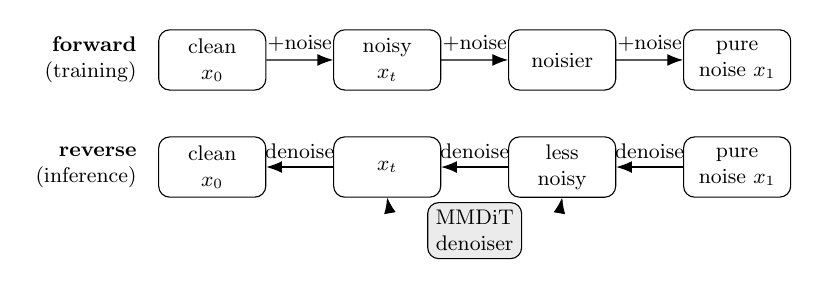
\begin{tikzpicture}[scale=0.85, transform shape, 
  font=\small,
  box/.style={draw, rounded corners, minimum width=1.6cm, minimum height=0.9cm, align=center},
  net/.style={draw, fill=black!8, rounded corners, minimum width=1.4cm, minimum height=0.7cm, align=center},
  >={Latex[length=2mm]}]
% top row: forward / noising (training)
\node[box] (a0) at (0,1.6) {clean\\$x_0$};
\node[box,right=1.0cm of a0] (a1) {noisy\\$x_t$};
\node[box,right=1.0cm of a1] (a2) {noisier};
\node[box,right=1.0cm of a2] (a3) {pure\\noise $x_1$};
\draw[->] (a0)--(a1) node[midway,above]{$+$noise};
\draw[->] (a1)--(a2) node[midway,above]{$+$noise};
\draw[->] (a2)--(a3) node[midway,above]{$+$noise};
\node[left=0.2cm of a0, align=right] {\textbf{forward}\\(training)};
% bottom row: reverse / denoising (inference)
\node[box] (b3) at (a3|-0,0) {pure\\noise $x_1$};
\node[box,left=1.0cm of b3] (b2) {less\\noisy};
\node[box,left=1.0cm of b2] (b1) {$x_t$};
\node[box,left=1.0cm of b1] (b0) {clean\\$x_0$};
\node[net] (net) at ($(b2)!0.5!(b1)+(0,-0.95)$) {MMDiT\\denoiser};
\draw[->] (b3)--(b2) node[midway,above]{denoise};
\draw[->] (b2)--(b1) node[midway,above]{denoise};
\draw[->] (b1)--(b0) node[midway,above]{denoise};
\draw[->,dashed] (net.north -| b2) to[bend left=10] (b2.south);
\draw[->,dashed] (net.north -| b1) to[bend right=10] (b1.south);
\node[left=0.2cm of b0, align=right] {\textbf{reverse}\\(inference)};
\end{tikzpicture}
\caption{The two directions of a diffusion model. Training adds noise to
real data in known amounts so the network can learn to reverse one step;
inference starts from pure noise and applies the learned reverse step
(the MMDiT denoiser) repeatedly to produce a new sample.}
\label{fig:diffusion-overview}
\end{figure}

\subsection{The forward process: how noise is added (used only in training)}

To teach the network to remove noise, we first need examples of noisy
data \emph{paired with} the clean original. These are manufactured by the
\textbf{forward process}: take a real clean image from the training set
and progressively corrupt it with random Gaussian noise. After enough
steps the image is indistinguishable from pure static.

Crucially, because \emph{we} are the ones adding the noise, we know
exactly how much was added at every step. A clean sample $x_0$ and a noise
level $t$ (think of $t$ as ``how far along the corruption we are'', from
$0$ = clean to $1$ = pure noise) give a noisy sample

\[
x_t \;=\; (1-t)\,x_0 \;+\; t\,\epsilon,
\qquad \epsilon \sim \mathcal{N}(0, I),
\]

where $\epsilon$ is the random noise. This is a simplified
\emph{flow-matching}~\cite{lipman2023flowmatching} (rectified-flow~%
\cite{liu2023rectifiedflow}) form of the forward
process~\cite{esser2024sd3}, which is the variant the Flux/Open-Sora family
uses; the exact schedule differs between diffusion formulations --- the
original \emph{denoising-diffusion} formulation~\cite{ho2020ddpm} adds noise
on a different schedule --- but the principle is identical. The key point for
this report is that the forward process is \textbf{cheap arithmetic with
no neural network in it} --- it is only used during training to make
training examples, and it never runs at inference time.

\subsection{The reverse process: how the network denoises}

The expensive, learned part is the \textbf{reverse process}. We want a
network that, given a noisy $x_t$ and the noise level $t$, predicts how to
step back towards the clean image --- in the flow-matching formulation it
predicts the \emph{velocity} $v_\theta(x_t, t)$ that points from the noisy
sample towards the clean one. This network is the \textbf{denoising
backbone}, and in modern text-to-video systems it is exactly the MMDiT
that this whole report is about.

Two extra inputs make the generation controllable and are fed to the
backbone alongside the noisy sample:

\begin{itemize}
\item the \textbf{noise level $t$}, so the network knows how corrupted its
input is (heavy denoising early, gentle touch-ups late);
\item the \textbf{text prompt}, encoded into a sequence of vectors, so the
network produces \emph{the video the user asked for} rather than an
arbitrary one. This is what makes the model \emph{multimodal} --- it
consumes both the image/video tokens and the text tokens at once.
\end{itemize}

\subsection{Training, step by step}
\label{sec:training-loop}

Training repeats the following loop millions of times. For one training
example:

\begin{enumerate}
\item Take a clean sample $x_0$ from the dataset and its text caption.
\item Pick a random noise level $t$ and a random noise $\epsilon$, and
build the noisy sample $x_t$ using the forward process above. Because we
chose $\epsilon$ and $t$, we know the \emph{true} answer the network
should produce (the target velocity).
\item \textbf{Forward pass.} Run the backbone $v_\theta(x_t, t, \text{text})$
to get the network's prediction.
\item \textbf{Loss.} Compare the prediction to the known true answer with a
simple squared-error \emph{loss} --- a single number measuring how wrong
the network was.
\item \textbf{Backward pass.} Compute, for every one of the network's
millions of weights, how a small change to that weight would change the
loss. These are the \emph{gradients}, obtained by \emph{backpropagation}
(the chain rule applied through the network, run in reverse).
\item \textbf{Optimiser step.} Nudge every weight a little in the
direction that reduces the loss. We use the \textbf{AdamW} optimiser,
which keeps a running average of recent gradients to make these nudges
smoother and more stable.
\end{enumerate}

Steps 3--6 are the four ingredients that matter for hardware, and they map
directly onto the three things this report implements and measures:
\textbf{the forward pass}, \textbf{the backward pass}, and \textbf{the
AdamW optimiser step}. The forward pass is just the network run normally;
the backward pass runs roughly twice the arithmetic of the forward (it
computes a gradient for both the inputs and the weights of every
operation); and the optimiser step is a comparatively small element-wise
update. All three are explained at the kernel level in
Chapter~\ref{ch:implementation}.

% FIGURE TODO fig:training-loop --- a labelled cycle:
%   data+text -> [add noise] -> x_t -> [FORWARD: MMDiT] -> prediction
%   -> [loss vs known target] -> [BACKWARD: gradients] -> [AdamW: update weights]
%   -> back to MMDiT. Mark which arrows are forward / backward / optimiser.
\begin{figure}[t]
\centering
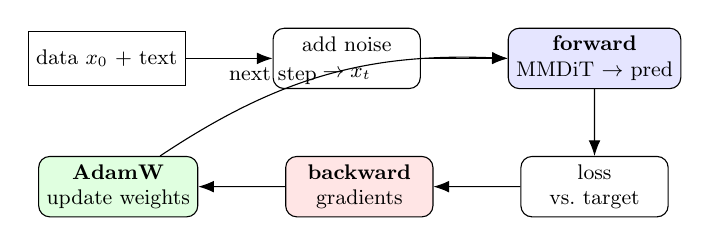
\begin{tikzpicture}[scale=0.85, transform shape, 
  font=\small,
  pstep/.style={draw, rounded corners, minimum width=2.2cm, minimum height=0.9cm, align=center},
  fwd/.style={draw, rounded corners, minimum width=2.2cm, minimum height=0.9cm, align=center, fill=blue!10},
  bwd/.style={draw, rounded corners, minimum width=2.2cm, minimum height=0.9cm, align=center, fill=red!10},
  opt/.style={draw, rounded corners, minimum width=2.2cm, minimum height=0.9cm, align=center, fill=green!12},
  data/.style={draw, minimum width=2.2cm, minimum height=0.8cm, align=center},
  >={Latex[length=2mm]}]
\node[data] (data) {data $x_0$ + text};
\node[pstep, right=1.3cm of data] (noise) {add noise\\$\to x_t$};
\node[fwd, right=1.3cm of noise] (fwd) {\textbf{forward}\\MMDiT $\to$ pred};
\node[pstep, below=1.0cm of fwd] (loss) {loss\\vs.\ target};
\node[bwd, left=1.3cm of loss] (bwd) {\textbf{backward}\\gradients};
\node[opt, left=1.3cm of bwd] (opt) {\textbf{AdamW}\\update weights};
\draw[->] (data)--(noise);
\draw[->] (noise)--(fwd);
\draw[->] (fwd)--(loss);
\draw[->] (loss)--(bwd);
\draw[->] (bwd)--(opt);
\draw[->] (opt) to[bend left=18] node[midway,left]{next step} (fwd.west|-fwd);
\end{tikzpicture}
\caption{One training step. The three stages implemented and measured in
this report --- \textcolor{blue!60!black}{forward pass},
\textcolor{red!60!black}{backward pass}, and
\textcolor{green!45!black}{AdamW optimiser step} --- are highlighted.}
\label{fig:training-loop}
\end{figure}

\subsection{Inference, step by step}
\label{sec:inference-loop}

Once trained, generating a new video does \emph{not} use the dataset, the
loss, the backward pass, or the optimiser at all. It only runs the forward
pass of the backbone, repeatedly:

\begin{enumerate}
\item Start from \textbf{pure random noise} $x_1$ --- the same Gaussian
static the forward process would have ended at.
\item Encode the user's text prompt into token vectors.
\item \textbf{Denoising loop.} For each of a fixed number of steps
(typically a few tens), from $t=1$ down towards $t=0$: run the backbone
forward to predict the velocity at the current noise level, and use it to
take one small step that makes the sample slightly cleaner.
\item After the last step, $x_0$ is a brand-new clean video matching the
prompt.
\end{enumerate}

The single most important fact about inference, for this project, is that
\textbf{the backbone runs once per denoising step}, and there are many
steps. There is also a second multiplier hiding inside each step:
\textbf{classifier-free guidance (CFG)}~\cite{ho2022cfg}. To steer the output
towards the prompt, the sampler does not evaluate the backbone once per step
but evaluates it on \emph{three} conditioning versions of the same latent ---
fully conditioned, text-dropped, and image-dropped --- and linearly combines
the three predictions to sharpen the result (Open-Sora uses a double CFG,
one guidance weight for the text condition and one for the image condition).
These three versions are stacked into the batch dimension and run through the
backbone in \emph{one} batched forward, so each denoising step is a single
backbone forward of effective batch~3. A generation of $S$ steps therefore
evaluates the backbone $3S$ times: at Open-Sora's $S=50$ this is
$3\times 50 = \mathbf{150}$ backbone evaluations, batched into 50 forwards.
This step count $\times$ CFG product is why a diffusion model's inference
cost is so much higher than a language model's --- a single prompt costs
${\sim}150$ full backbone passes rather than one --- and why the per-pass
efficiency of the backbone is what determines whether the whole system is
affordable.
Because inference is the latency- and energy-critical path that users pay
for repeatedly, it is run at \textbf{low precision}
(Section~\ref{sec:quant}); training, which happens once and must be
numerically robust, is run at \textbf{high precision}. The bridge between
them --- adapting a high-precision-trained model to run at low precision
--- is a short \emph{fine-tuning} stage that reuses the very same backward
and optimiser machinery as training.

\section{The multimodal diffusion transformer (MMDiT)}
\label{sec:mmdit}

\subsection{From transformer to diffusion transformer}

The denoising backbone is a \textbf{transformer}, the same family of
network behind modern language models~\cite{vaswani2017attention}. A
transformer operates on a \emph{sequence of tokens}, where each token is a
vector, and its central operation is \textbf{attention}: every token looks
at every other token and pulls in information from the ones relevant to it.
Stacking many such \emph{blocks} lets the network build up a rich,
context-aware representation of the whole sequence.

To use a transformer for image or video diffusion, the image is first cut
into a grid of small patches, and each patch becomes one token --- so a
picture turns into a sequence, exactly the form a transformer expects.
A transformer used this way as a diffusion backbone is called a
\textbf{diffusion transformer (DiT)}~\cite{peebles2023dit}.

\subsection{What ``multimodal'' adds}

A plain DiT handles one modality: the image tokens. A text-to-video model
must also consume the \textbf{text prompt}, which is a second sequence of
tokens of a completely different nature. The \textbf{multimodal} diffusion
transformer (MMDiT) is the design that lets image tokens and text tokens
interact properly. Rather than gluing the two together crudely, the MMDiT
lets both streams attend to each other inside a single shared attention,
so the image can be shaped by the words and vice versa.

The MMDiT design was popularised by the Flux / Stable Diffusion~3 family,
where the joint two-stream attention was introduced~\cite{esser2024sd3},
and has since become one of the most widely reused backbones in generative
AI. The same structure powers text-to-image and text-to-video diffusion
models such as \textbf{Open-Sora}~\cite{opensora2024}; it appears in large
multimodal generation models such as \textbf{Qwen}~\cite{qwenimage2025};
and it underpins a growing number of robotics
\textbf{vision--language--action (VLA)} models~\cite{openvla2024}, where the
``image'' tokens are camera frames and the ``text'' tokens are
instructions. Accelerating
the MMDiT therefore pays off across a wide span of modern systems, not
just video generation --- which is the central motivation of this report.

\subsection{How conditioning enters: modulation}

The backbone must be told the noise level $t$ and a global summary of the
prompt. The MMDiT injects these through \textbf{modulation} (also called
adaptive layer-norm, or adaLN): the conditioning is turned into a small
set of per-block scale-and-shift parameters that stretch, offset, and gate
the token vectors inside each block. This is a cheap, element-wise
mechanism, but it is how every block ``knows'' how much denoising to do
and what the prompt is about.

\subsection{The pieces inside a block}

Every block of the MMDiT is built from the same small set of operations,
which recur throughout the report:

\begin{itemize}
\item \textbf{Normalisation} (layer-norm / RMS-norm): rescales each token
vector to a stable range so the arithmetic stays well-behaved.
\item \textbf{Modulation}: applies the conditioning scale/shift/gate
described above.
\item \textbf{Linear layers (GEMMs)}: large dense matrix multiplications
that mix information across a token's features. These are the bulk of the
compute.
\item \textbf{Q/K/V projection and QK-normalisation}: produce the
\emph{query}, \emph{key}, and \emph{value} vectors used by attention, and
normalise queries and keys for stability.
\item \textbf{Rotary position embedding (RoPE)}: encodes \emph{where} each
token sits (its position in the image grid or text) by rotating the query
and key vectors, so attention is position-aware.
\item \textbf{Attention}: the all-to-all mixing operation, computed here
with the memory-efficient \emph{flash-attention} algorithm.
\item \textbf{GELU and the MLP}: a two-layer feed-forward network with a
GELU non-linearity that processes each token independently.
\item \textbf{Residual connections}: each block adds its result back onto
its input, which keeps very deep stacks trainable.
\end{itemize}

Of these, the \textbf{linear layers} and the \textbf{attention} are the
matrix-heavy operations that dominate cost; the rest are lighter
element-wise or per-row operations handled by the accelerator's vector
unit.

\section{Open-Sora: the benchmark model}
\label{sec:opensora}

To measure the MMDiT on a real workload rather than a synthetic one, this
report uses \textbf{Open-Sora}, an open-source text-to-video model, as its
benchmark. Open-Sora takes a text prompt and produces a short video clip;
every block is run at Open-Sora's true dimensions and, for the accuracy
study, with its real trained weights. Understanding what surrounds the
MMDiT inside Open-Sora makes clear why this report concentrates on the
MMDiT alone.

\subsection{What Open-Sora is made of}

A text-to-video generation in Open-Sora is a pipeline of three kinds of
component:

\begin{itemize}
\item \textbf{Text encoders} (e.g.\ T5 and CLIP) turn the user's prompt
into the sequence of text-token vectors the backbone conditions on. They
run \emph{once} per generation.
\item \textbf{The MMDiT denoising backbone} --- the Flux MMDiT described
above --- is run inside the denoising loop, \emph{many tens of times} per
generation. It operates in a compressed \emph{latent} space rather than on
raw pixels~\cite{rombach2022ldm}, which is what keeps the token sequence (and
therefore the cost) manageable.
\item \textbf{The VAE} (variational autoencoder) sits at the boundary
between that latent space and actual pixels. Its \emph{decoder} is run
\emph{once} at the very end to expand the final clean latent the MMDiT
produced into the full-resolution video.
\end{itemize}

% FIGURE: real generated inference-flow figure from the old report
\begin{figure}[t]
\centering
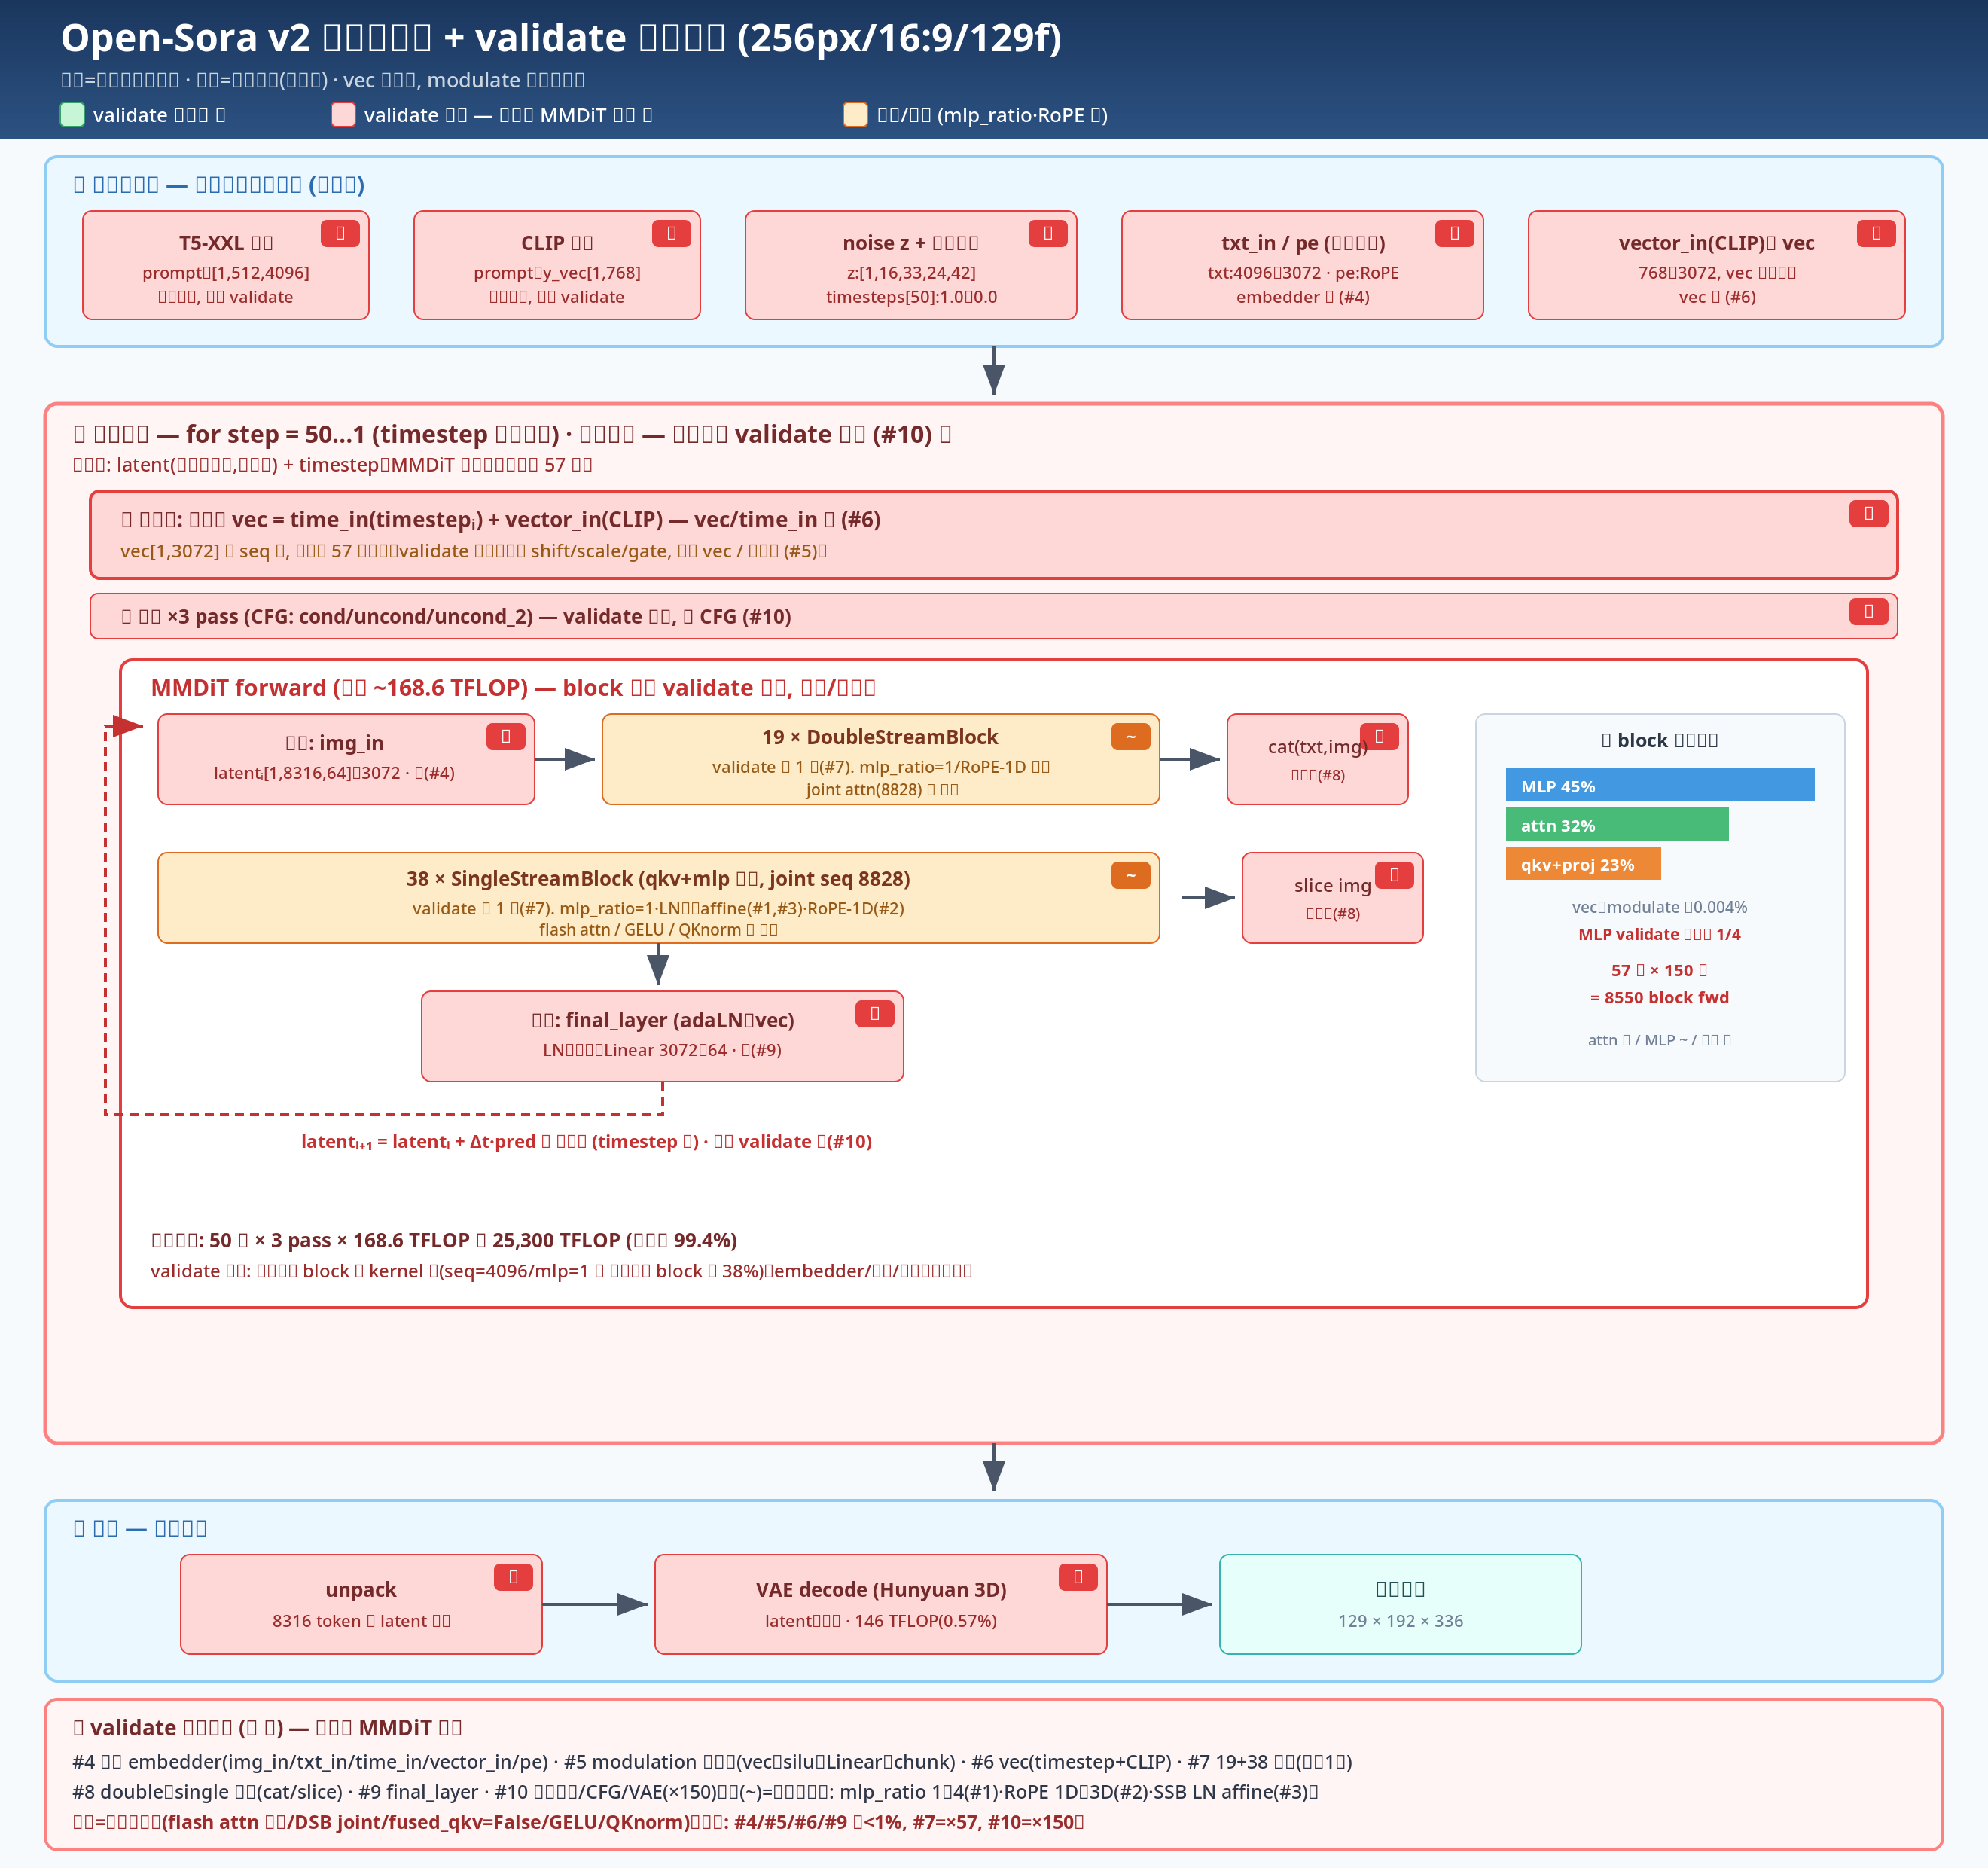
\includegraphics[width=0.92\linewidth,keepaspectratio]{transactional_emulator/testbench/MMDIT_INFERENCE_FLOW.png}
\caption{Open-Sora inference flow. The text encoders and the VAE decoder
run once each; the MMDiT backbone (centre) runs once per denoising step,
many tens of times per generation, and dominates the total cost.}
\label{fig:opensora-flow}
\end{figure}

\subsection{The role of the MMDiT --- and why the VAE is separate}

The MMDiT is the part of Open-Sora that actually performs the generation:
it is the learned denoiser that, step by step, turns noise into a coherent
video matching the prompt. Everything else is support around it. In
particular, the \textbf{VAE is a distinct model with its own, separate
training} --- it is trained independently to compress video into the
latent space and back, and in practice the VAE is often borrowed from
\emph{another} model entirely and reused, rather than trained alongside the
MMDiT. The two are only loosely coupled: the MMDiT learns to denoise in
whatever latent space the VAE defines, but the VAE itself is not part of
the backbone this report accelerates. This is why ``accelerating
Open-Sora'' reduces, almost exactly, to ``accelerating the MMDiT.''

\subsection{Where the compute is: the whole-model breakdown}
\label{sec:compute-breakdown}

This reduction is not a hand-wave; it is what a direct count of the
arithmetic shows. Counting the floating-point operations (FLOPs) across a
full generation --- roughly fifty denoising timesteps, each with a few
backbone passes --- the MMDiT overwhelmingly dominates:

\begin{center}
\begin{tabular}{@{}llr@{}}
\toprule
Stage & FLOP (full generation) & Share \\
\midrule
\textbf{MMDiT forward (the backbone)} & \textbf{25{,}300 TFLOP} & \textbf{99.40\%} \\
VAE decode (once) & 146 TFLOP & 0.58\% \\
Text encoders / embedder / unpack (once) & ${\sim}5$ TFLOP & 0.02\% \\
\bottomrule
\end{tabular}
\end{center}

A single MMDiT forward pass is about $168.6$\,TFLOP; multiplied by the
${\sim}150$ times it is invoked across a generation, this becomes the
$25{,}300$\,TFLOP that defines the inference cost. The text encoders and
the VAE decoder, run only once each, are together under $0.6\%$ of the
total and are not worth optimising. \textbf{Accelerating Open-Sora is
therefore equivalent to accelerating the MMDiT forward pass}, which is
exactly what this report does. The same conclusion is what makes the work
general: any model built on the MMDiT --- text-to-image, Qwen-style
multimodal, or a VLA policy --- spends essentially all of its compute in
the very block types analysed here.

\section{The two block types: single-stream and double-stream}
\label{sec:blocks}

The MMDiT is a stack of transformer blocks of two kinds. At Open-Sora's
real dimensions a single MMDiT pass is built almost entirely from these
two block types:

\begin{itemize}
\item \textbf{38 single-stream blocks (SSB)} --- two-thirds of the pass;
\item \textbf{19 double-stream blocks (DSB)} --- one-third of the pass;
\item a tiny output head (the \emph{final layer}) that is under 0.2\% of
the work and can be ignored for cost purposes.
\end{itemize}

A single-stream and a double-stream block cost almost the same per block
(both about $2.96$\,TFLOP at Open-Sora dimensions), so with twice as many
single-stream blocks, the SSB carries roughly \textbf{two-thirds of the
entire MMDiT pass} and the DSB the remaining third. Together they are
\textbf{99.8\%} of every pass, which is why the entire acceleration effort
in this report targets exactly these two block types. They are built from
the same set of operations listed above, so any improvement to one
transfers directly to the other.

\subsection{The single-stream block (SSB)}

The single-stream block runs \textbf{one fused stream} over the
already-concatenated joint sequence of image and text tokens (about
$9{,}216$ tokens at Open-Sora's dimensions). Its data-flow is a single
straight pipeline: one normalisation, modulation, a combined Q/K/V linear,
QK-normalisation, RoPE, flash attention, a fused projection-plus-MLP
linear, and a residual add back onto the input. Because the image and text
tokens already sit in one sequence, every operation sees both at once.

\begin{figure}[t]
\centering
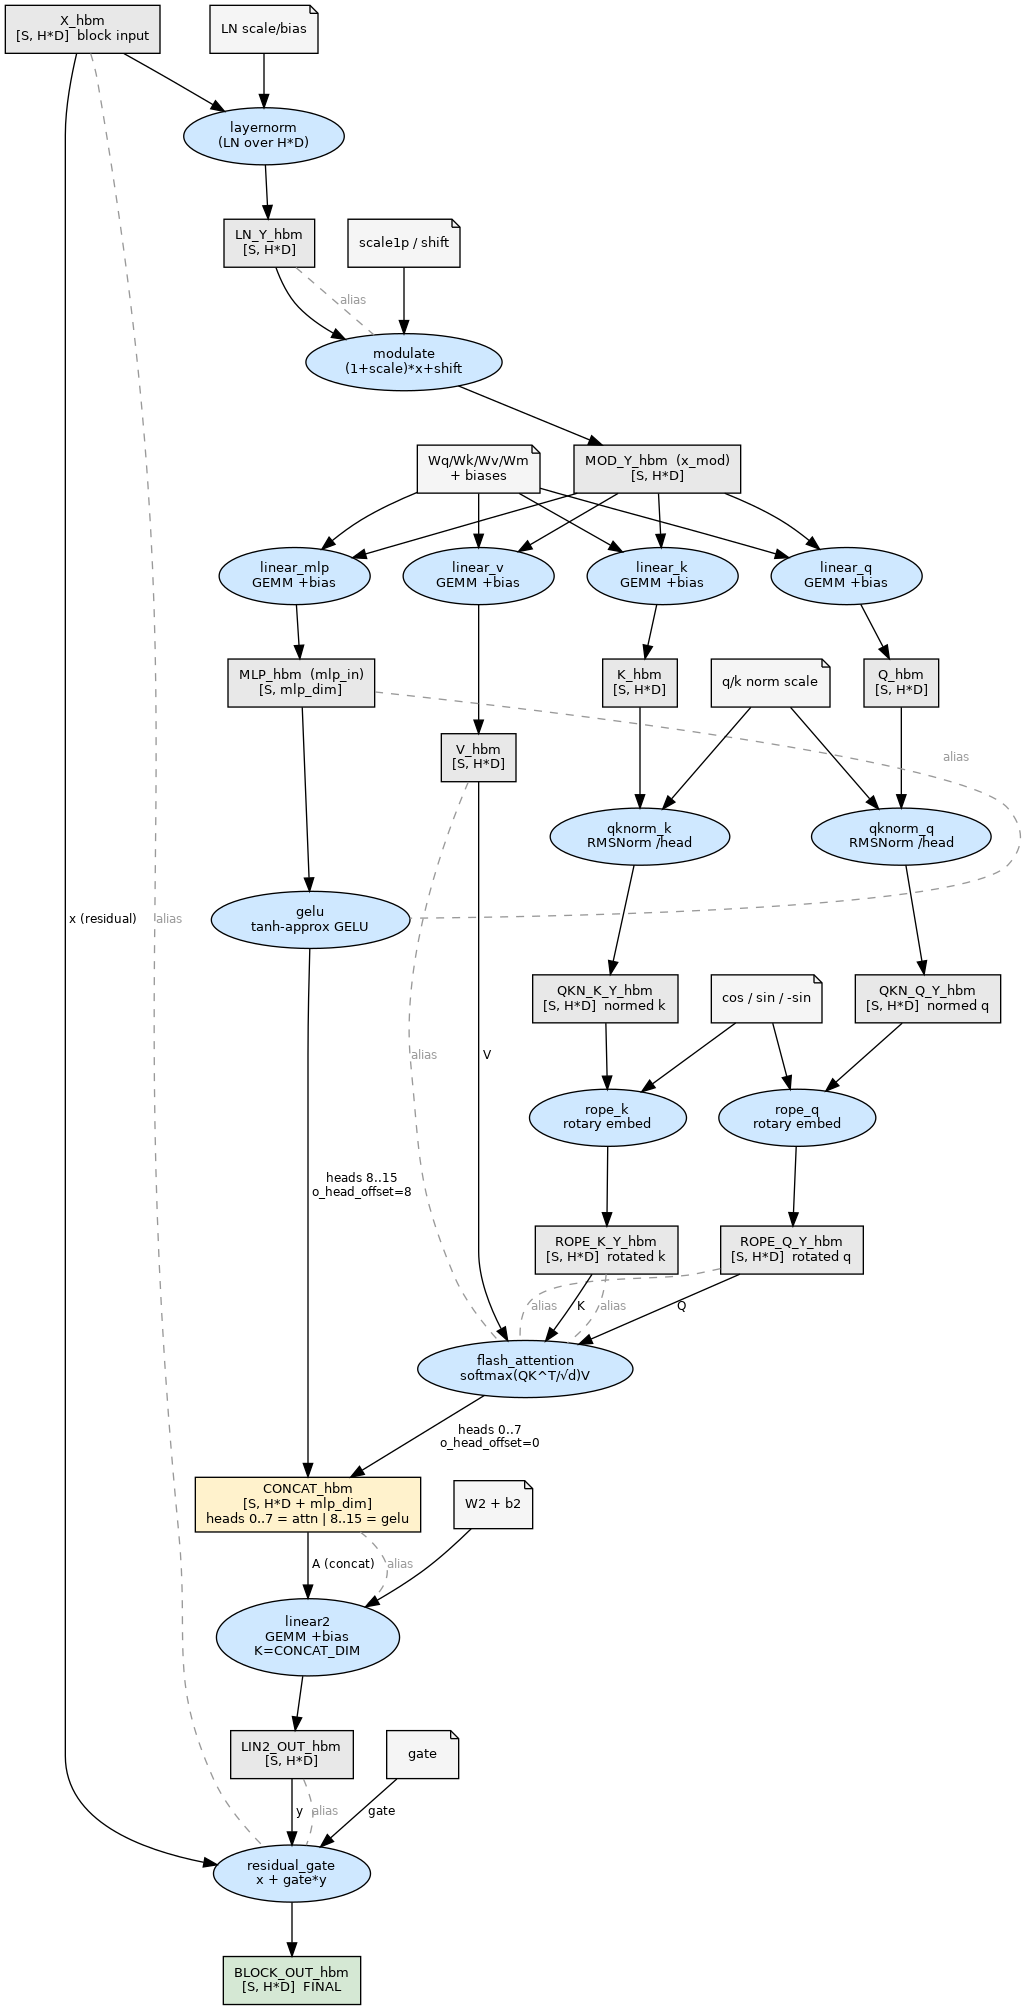
\includegraphics[width=0.62\linewidth,keepaspectratio]{transactional_emulator/testbench/single_stream_block_graph.png}
\caption{Single-stream block (SSB) data-flow graph: one fused pipeline over
the joint image+text sequence (norm $\to$ modulate $\to$ QKV linear $\to$
QK-norm $\to$ RoPE $\to$ flash attention $\to$ fused proj+MLP $\to$
residual). The flash attention is the heaviest single kernel.}
\label{fig:ssb}
\end{figure}

\subsection{The double-stream block (DSB)}

The double-stream block runs \textbf{two independent streams} --- one for
image tokens, one for text tokens --- each with \emph{its own separate
weights}. Each stream first runs its own pre-attention path (norm,
modulate, Q/K/V linear, QK-norm, RoPE). The two streams are then
\textbf{concatenated into one joint sequence for a single shared flash
attention}, so image and text mix; afterwards the result is split back
apart and each stream runs its own post-attention path (projection, MLP,
residual). It is, in effect, two single-stream pipelines that meet in the
middle for one joint attention.

\begin{figure}[p]
\centering
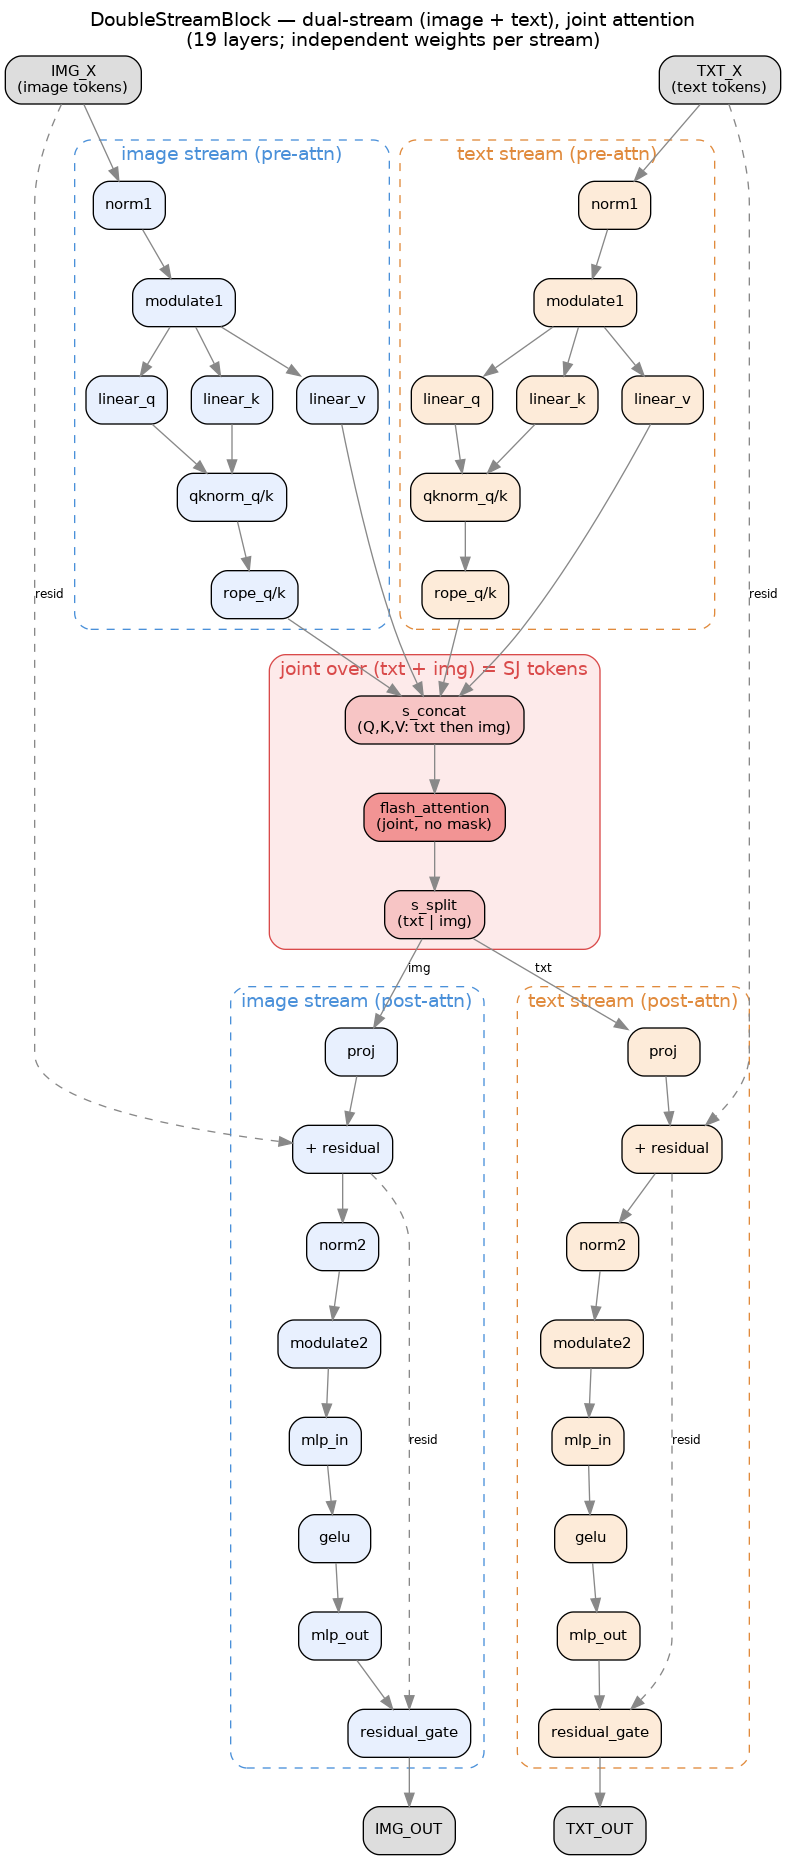
\includegraphics[height=0.82\textheight,keepaspectratio]{transactional_emulator/testbench/double_stream_block_graph.png}
\caption{Double-stream block (DSB) data-flow graph: separate image and text
streams (each with its own weights) that join for a single shared flash
attention, then split again. The shared attention is where the two
modalities interact.}
\label{fig:dsb}
\end{figure}

\paragraph{Why attention dominates both.} In both block types the heaviest
single kernel is the \textbf{joint flash attention}. Because the MMDiT is
not autoregressive, this is \emph{full bidirectional} attention over the
long joint sequence --- every token attends to every other, with no causal
mask and no key/value cache. The cost of attention grows with the square
of the sequence length, and with about ten thousand tokens this term is
large, which is why attention drives most of the matrix and vector work in
either topology.

\section{Inside a block: the kernels}
\label{sec:kernels}

This section opens up a block into the individual \emph{kernels} it is
built from --- the elementary operations the accelerator actually executes
--- and gives, for each, a short piece of pseudocode and its compute cost.
We do this twice: once for the \textbf{forward} pass (used in both
inference and training) and once for the \textbf{backward} pass and
optimiser (used only in training). All FLOP figures are for one
single-stream block at Open-Sora's real dimensions: a joint sequence of
$S = 9216$ tokens, hidden width $\mathrm{HD} = 3072$, $\mathrm{HEAD}=24$
attention heads of width $\mathrm{HLEN}=128$, and an MLP hidden width of
$4\,\mathrm{HD} = 12288$. We count a multiply--accumulate as 2 FLOP, so a
matrix product of an $m\times k$ by a $k\times n$ matrix costs $2mkn$
FLOP; the double-stream block runs essentially the same kernels twice (once
per stream) around one shared attention, so its per-kernel costs follow
directly.

It is useful to keep one distinction in mind throughout: the
\textbf{matrix kernels} (the linear layers and attention) are large dense
matrix multiplies that run on the systolic array and account for almost
all of the FLOPs, whereas the \textbf{vector kernels} (normalisation,
modulation, RoPE, GELU, the residual gate) are light, element-wise or
per-row operations that run on the vector unit and contribute a negligible
share of the arithmetic but are essential for correctness.

\subsection{Forward kernels}
\label{sec:fwd-kernels}

A forward pass through the single-stream block is the following sequence
of kernels, in order. The data-flow graph in Figure~\ref{fig:ssb} shows
the same sequence visually.

\paragraph{1. LayerNorm.} \emph{Why it is here:} a deep stack of blocks is
only trainable if the numbers flowing through it stay in a stable range; if
activations are free to grow or shrink block by block, gradients explode or
vanish and training fails. LayerNorm~\cite{ba2016layernorm} fixes this by
rescaling each token vector to zero mean and unit variance before the heavy
arithmetic, then applying a learned scale and shift so the network can still
choose the magnitude it wants. It reduces along the hidden axis (a per-row
mean and variance) and is a vector kernel.

\begin{algorithm}[H]
\DontPrintSemicolon
\KwIn{$X \in \mathbb{R}^{S\times \mathrm{HD}}$; scale $\gamma$, shift $\beta$}
\For{each row $i$}{
  $\mu_i \leftarrow \mathrm{mean}_j X_{ij}$\;
  $\sigma^2_i \leftarrow \mathrm{mean}_j (X_{ij}-\mu_i)^2$\;
  $Y_{ij} \leftarrow (X_{ij}-\mu_i)\,/\sqrt{\sigma^2_i+\epsilon}\;\cdot\gamma_j + \beta_j$\;
}
\caption{LayerNorm (vector; ${\sim}S\!\cdot\!\mathrm{HD}$ elements)}
\end{algorithm}

\paragraph{2. Modulation (adaLN).} \emph{Why it is here:} every block needs
to be told two things --- how noisy its input currently is, and what the
prompt is about --- and must be able to react differently at different
noise levels. Rather than feed this conditioning in as extra tokens,
adaptive layer-norm (adaLN) turns it into a per-block
\emph{scale-and-shift} applied right after normalisation,
$Y = (1+\text{scale})\odot X + \text{shift}$. This is the mechanism the DiT
design showed to be both cheap and effective for injecting
conditioning~\cite{peebles2023dit}; in the MMDiT it is what makes each
block noise-level- and prompt-aware. It is a cheap element-wise vector
kernel.

\paragraph{3. Q, K, V and MLP-in linear layers.} \emph{Why they are here:}
these are the block's learned ``mixing'' across a token's features. The
Q/K/V projections turn each token into the three roles attention needs ---
a \emph{query} (what am I looking for), a \emph{key} (what do I offer), and
a \emph{value} (what I pass on if attended to) --- while the MLP-in
projection lifts the token into a wider space where the non-linearity can
act. They are dense matrix multiplies $Y = X W^\top + b$ and are the first
of the big matrix kernels that carry the bulk of the compute.

\begin{algorithm}[H]
\DontPrintSemicolon
\KwIn{$X \in \mathbb{R}^{S\times \mathrm{HD}}$; weight $W \in \mathbb{R}^{N\times \mathrm{HD}}$; bias $b$}
$Y \leftarrow X\,W^\top + b$ \tcp*{$S\times N$ output, tiled onto the systolic array}
\caption{Linear layer ($Y=XW^\top+b$)}
\end{algorithm}

For Q/K/V, $N=\mathrm{HD}=3072$; for the MLP input, $N=4\,\mathrm{HD}=12288$.

\paragraph{4. QK-normalisation.} Its role is stability. The dot products
inside attention can grow large enough to make the softmax numerically
unstable, so each query and key vector is first rescaled to a controlled
magnitude. This uses RMS-normalisation~\cite{zhang2019rmsnorm} --- a
cheaper variant of LayerNorm that divides by the root-mean-square without
subtracting the mean --- applied once per head. It keeps the attention
scores in a well-behaved range and is a cheap per-row vector kernel.

\paragraph{5. RoPE --- giving attention a sense of position.} Attention,
as defined above, is completely \emph{order-blind}: the score between two
tokens depends only on their content, not on \emph{where} they sit. Yet
position is essential --- in a video the same patch means something
different at the top-left of an early frame than at the bottom-right of a
later one, and in text the order of words carries the meaning. Some
mechanism must tell attention where each token is.

Rotary Position Embedding (RoPE)~\cite{su2021roformer} is an elegant way to
do this. Instead of
\emph{adding} a position signal to the token (the older approach, which
the network then has to disentangle), RoPE \emph{rotates} each query and
key vector by an angle proportional to that token's position. Pairs of
coordinates within the vector are treated as points in a plane and turned
by position-dependent angles --- early tokens are barely rotated, later
tokens turned further. The beauty of the scheme is what happens when two
such vectors are then compared inside attention: because a dot product of
two rotated vectors depends only on the \emph{difference} of their
rotation angles, the attention score between token $i$ and token $j$
automatically becomes a function of their \emph{relative} position
$i-j$. In other words, RoPE injects absolute position into each vector
yet makes attention respond to relative distance --- and it does so
without any extra parameters, without changing the size of anything, and
without a separate term to be learned. Applied once to the queries and
once to the keys just before attention, it is a light vector kernel whose
effect on the model's quality is large.

\paragraph{6. GELU --- the non-linearity.} Between its two MLP layers the
block needs a non-linear function; without one, two stacked linear layers
would collapse into a single linear map and the MLP would add nothing.
GELU~\cite{hendrycks2016gelu} is the smooth non-linearity used here: it
passes large positive values through almost unchanged and suppresses
negative ones gently rather than clipping them hard, which makes its
gradient smoother than a hard-gating ReLU. It is applied element-wise to every MLP hidden
activation and is a vector kernel.

\paragraph{7. Attention.} The all-to-all mixing step, and the single
heaviest kernel in the block. For each of the 24 heads it forms the
attention scores $QK^\top$, applies a softmax over the sequence, and mixes
the values with $PV$. In its plain mathematical form the kernel is just
three steps per head:

\begin{algorithm}[H]
\DontPrintSemicolon
\KwIn{$Q,K,V \in \mathbb{R}^{S\times \mathrm{HLEN}}$ per head}
\For{each head}{
  $S \leftarrow Q K^\top \cdot \text{scale}$ \tcp*{scores, $S\times S$ (matrix)}
  $P \leftarrow \mathrm{softmax}(S)$ \tcp*{row-wise softmax (vector)}
  $O \leftarrow P\,V$ \tcp*{value mix, $S\times \mathrm{HLEN}$ (matrix)}
}
\caption{Attention (full bidirectional, no mask, no KV cache)}
\end{algorithm}

\noindent This is the operation being computed. Because the full
$S\times S$ score matrix is far too large to store at $S=9216$, the actual
implementation never forms it explicitly; it uses the memory-efficient
\emph{flash-attention} algorithm~\cite{dao2022flashattention}, which streams
over the sequence in tiles and fuses the softmax into the matrix
multiplies. That optimisation belongs
to the implementation and is described in
Chapter~\ref{ch:implementation}; here we treat it as the attention kernel
defined above.

\paragraph{8. Concat.} Joins the attention output and the GELU'd MLP
activations along the feature axis into one $5\,\mathrm{HD}$-wide tensor ---
a pure data-movement vector kernel, no arithmetic.

\paragraph{9. Output linear (proj+MLP-out).} A single fused matrix multiply
that projects the concatenated $5\,\mathrm{HD}$ tensor back to the hidden
width $\mathrm{HD}$. This is the largest single linear in the block because
its contraction dimension is $5\,\mathrm{HD}=15360$.

\paragraph{10. Residual gate.} Adds the block's result back onto its input
through a learned gate, $\text{out} = X + \text{gate}\odot Y$ --- a cheap
element-wise vector kernel that closes the residual connection.

\begin{table}[t]
\centering
\caption{Forward kernels of one single-stream block at Open-Sora
dimensions ($S{=}9216$, $\mathrm{HD}{=}3072$, 24 heads). Matrix kernels
dominate; vector kernels are individually below ${\sim}0.05$\,TFLOP.}
\label{tab:fwd-kernels}
\begin{tabular}{@{}llr@{}}
\toprule
Kernel & Type & FLOP \\
\midrule
LayerNorm & vector & negligible \\
Modulation & vector & negligible \\
Linear Q / K / V (each) & matrix & 0.17\,TFLOP \\
Linear MLP-in ($\mathrm{HD}\!\to\!4\mathrm{HD}$) & matrix & 0.70\,TFLOP \\
QK-norm (RMS, $\times 2$) & vector & negligible \\
RoPE ($\times 2$) & vector & negligible \\
GELU & vector & negligible \\
Attention ($QK^\top$ + $PV$) & matrix & 1.04\,TFLOP \\
Concat & vector (copy) & 0 \\
Output linear ($5\mathrm{HD}\!\to\!\mathrm{HD}$) & matrix & 0.87\,TFLOP \\
Residual gate & vector & negligible \\
\midrule
\textbf{Forward total} & & \textbf{${\sim}3.1$\,TFLOP} \\
\bottomrule
\end{tabular}
\end{table}

Table~\ref{tab:fwd-kernels} collects the costs. Two things stand out and
recur for the rest of the report: \textbf{attention is the single
biggest kernel} ($1.04$\,TFLOP, a third of the block), and \textbf{the
matrix kernels carry essentially all of the FLOPs} while the seven vector
kernels together are under a few percent. This is exactly the profile a
matrix accelerator is built for.

\subsection{Backward and optimiser kernels}
\label{sec:bwd-kernels}

Training adds two more stages on top of the forward pass: the
\textbf{backward pass}, which computes a gradient for every weight, and the
\textbf{optimiser step}, which uses those gradients to update the weights.
The backward pass runs the block ``in reverse'': it starts from the
gradient of the loss with respect to the block's output and propagates it
back through every kernel, in the opposite order, producing two gradients
at each linear layer.

% FIGURE TODO fig:ssb-bwd --- backward data-flow graph of the SSB:
%   reverse order, each fwd op replaced by its bwd kernel; the two grads
%   (dX, dW) split at each linear; the 5-GEMM flash-attention bwd; the
%   AdamW update consuming each dW. (To be generated like the fwd graph.)
\begin{figure}[t]
\centering
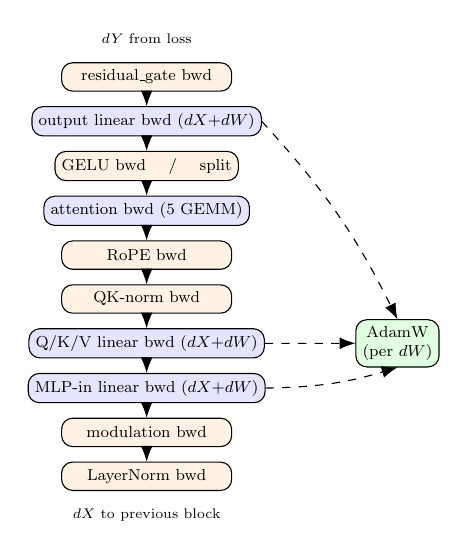
\begin{tikzpicture}[scale=0.72, transform shape, font=\footnotesize, node distance=2.6mm, >={Latex[length=2mm]},
  mat/.style={draw, rounded corners, minimum width=3.0cm, minimum height=0.5cm, align=center, fill=blue!10},
  vec/.style={draw, rounded corners, minimum width=3.0cm, minimum height=0.5cm, align=center, fill=orange!10},
  adam/.style={draw, rounded corners, minimum height=0.5cm, align=center, fill=green!12}]
% reverse-order chain (top = loss side, bottom = input side)
\node[vec] (rg) {residual\_gate bwd};
\node[mat, below=of rg] (l2) {output linear bwd ($dX{+}dW$)};
\node[vec, below=of l2] (gelu) {GELU bwd \quad / \quad split};
\node[mat, below=of gelu] (attn) {attention bwd (5 GEMM)};
\node[vec, below=of attn] (rope) {RoPE bwd};
\node[vec, below=of rope] (qkn) {QK-norm bwd};
\node[mat, below=of qkn] (qkv) {Q/K/V linear bwd ($dX{+}dW$)};
\node[mat, below=of qkv] (mlp) {MLP-in linear bwd ($dX{+}dW$)};
\node[vec, below=of mlp] (mod) {modulation bwd};
\node[vec, below=of mod] (ln) {LayerNorm bwd};
\foreach \a/\b in {rg/l2,l2/gelu,gelu/attn,attn/rope,rope/qkn,qkn/qkv,qkv/mlp,mlp/mod,mod/ln}
  \draw[->] (\a)--(\b);
\node[above=2mm of rg] {\scriptsize $dY$ from loss};
\node[below=2mm of ln] {\scriptsize $dX$ to previous block};
% AdamW consumes each dW
\node[adam, right=1.6cm of qkv] (adam) {AdamW\\(per $dW$)};
\draw[->,dashed] (l2.east) to[bend left=8] (adam.north);
\draw[->,dashed] (qkv.east) -- (adam.west);
\draw[->,dashed] (mlp.east) to[bend right=8] (adam.south);
\end{tikzpicture}
\caption{Backward (training) data-flow of the single-stream block. The
forward kernels are traversed in reverse; each linear (blue) splits into its
input-gradient and weight-gradient GEMMs, attention expands to five GEMMs,
the vector kernels (orange) give their Jacobians, and AdamW consumes each
weight gradient $dW$.}
\label{fig:ssb-bwd}
\end{figure}

\paragraph{The ``one forward, two backward'' rule.} The key fact about
backward cost is that every forward matrix multiply becomes \emph{two}
matrix multiplies on the way back. A linear layer $Y = X W^\top$ must
produce both the gradient flowing to its input and the gradient for its own
weights:

\begin{algorithm}[H]
\DontPrintSemicolon
\KwIn{output gradient $dY$; forward inputs $X$, weight $W$}
$dX \leftarrow dY\,W$ \tcp*{input gradient (matrix), contract $N$}
$dW \leftarrow dY^\top X$ \tcp*{weight gradient (matrix), contract $S$}
\caption{Linear backward (two GEMMs per forward linear)}
\end{algorithm}

This is why the backward pass costs roughly \textbf{twice} the forward in
matrix work. Each vector kernel likewise has a backward counterpart, but
those stay cheap. The full mapping is:

\begin{center}
\begin{tabular}{@{}lll@{}}
\toprule
Forward kernel & Backward kernel(s) & Cost \\
\midrule
Linear (Q/K/V, MLP, output) & \texttt{linear\_bwd\_dx} + \texttt{linear\_bwd\_dw} & 2 GEMMs each \\
Attention & \texttt{flash\_attention\_bwd} & 5 GEMMs \\
RoPE & \texttt{rope\_bwd} & 1 shuffle-GEMM \\
QK-norm (RMS) & \texttt{rmsnorm\_bwd} & vector \\
LayerNorm & \texttt{layernorm\_bwd} & vector \\
GELU & \texttt{gelu\_bwd} & vector \\
Modulation, residual gate & \texttt{affine\_bwd} & vector \\
\bottomrule
\end{tabular}
\end{center}

\paragraph{Attention backward.} Attention is the only kernel whose
backward is not a simple doubling: it expands into \textbf{five} matrix
multiplies to produce the gradients $dQ$, $dK$, and $dV$. As in the
forward pass, the implementation uses the flash-attention algorithm and
computes the scores in \emph{transposed} form so that four of the five
GEMMs need no transpose and only the final $dQ$ does, which matches the
accelerator's matrix-RAM layout (the implementation detail is in
Chapter~\ref{ch:implementation}):

\begin{algorithm}[H]
\DontPrintSemicolon
\KwIn{forward $Q,K,V$; output gradient $dO$; softmax stats $L,D$}
$S^\top \leftarrow K\,Q^\top \cdot \text{scale}$;\quad $P^\top \leftarrow \exp(S^\top - L)$\;
$dP^\top \leftarrow V\,dO^\top$\;
$dV \mathrel{+}= P^\top dO$ \tcp*{no transpose}
$dS^\top \leftarrow P^\top \odot (dP^\top - D)$\;
$dK \mathrel{+}= dS^\top Q$ \tcp*{no transpose}
$dQ \leftarrow (dS^\top)^\top K$ \tcp*{one transpose}
\caption{Attention backward (five head-fused GEMMs)}
\end{algorithm}

\paragraph{The vector backward kernels.} The remaining kernels each have a
backward that stays on the vector unit --- cheap relative to the matrix
work above, but needed for a correct gradient. They are worth stating
because each is the exact analytic derivative of its forward kernel, not an
approximation:

\begin{itemize}
\item \textbf{LayerNorm / RMS-norm backward.} Differentiating a
normalisation is not element-wise, because every output of a row depends on
the row's mean and variance. The exact input gradient therefore contains
two extra per-row reductions. For RMS-norm, with $\mathrm{inv}=1/\mathrm{rms}$,
\[
dx_i = \mathrm{inv}\,(dy_i\,g_i) \;-\; x_i\,\mathrm{inv}^3\,\tfrac{1}{H}\textstyle\sum_j dy_j\,g_j\,x_j,
\]
and LayerNorm backward has the analogous form with one more term for the
mean subtraction. Both reduce along the hidden axis and run as vector
kernels.
\item \textbf{RoPE backward.} Because a rotation is orthogonal, undoing it
is just rotating by the negative angle --- so the backward is the same
shuffle-and-multiply as the forward, run with the opposite sign. It costs
the same as the forward RoPE (a $1\times$, not $2\times$, kernel) and needs
no matrix multiply.
\item \textbf{GELU backward.} Element-wise: the incoming gradient is scaled
by the exact derivative of the GELU curve, $dx = dy\cdot\mathrm{gelu}'(x)$,
evaluated from the same $\exp$-based form as the forward.
\item \textbf{Affine backward (modulation, residual gate).} The forward is
an element-wise scale-and-shift, so the backward simply multiplies the
incoming gradient by that same scale --- the cheapest kernel of all, no
reduction and no matrix multiply.
\end{itemize}

\paragraph{Optimiser: AdamW.} After the backward pass has produced a
gradient $g$ for every weight, the optimiser updates the weights. We use
\textbf{AdamW}~\cite{loshchilov2019adamw}, which keeps two running averages
per weight --- a smoothed gradient $m$ and a smoothed squared gradient $v$
--- and steps each weight by a normalised amount, with weight decay applied
separately from the gradient step. It is a purely element-wise vector kernel, applied
once per weight tensor:

\begin{algorithm}[H]
\DontPrintSemicolon
\KwIn{weight $w$, gradient $g$, states $m,v$, step $t$}
$m \leftarrow \beta_1 m + (1-\beta_1)\,g$;\quad
$v \leftarrow \beta_2 v + (1-\beta_2)\,g^2$\;
$\hat m \leftarrow m/(1-\beta_1^t)$;\quad
$\hat v \leftarrow v/(1-\beta_2^t)$\;
$w \leftarrow w - \mathrm{lr}\,\hat m\,/(\sqrt{\hat v}+\epsilon)$\;
\caption{AdamW update (vector, element-wise per weight)}
\end{algorithm}

\noindent One hardware subtlety surfaces here: PLENA's vector unit has no
element-wise square root, so the $1/(\sqrt{\hat v}+\epsilon)$ term is
computed with a single Newton--Raphson reciprocal-square-root iteration
built from multiplies, adds, and a reciprocal. This and the other
ISA-level details are deferred to Chapter~\ref{ch:implementation}.

\begin{table}[t]
\centering
\caption{Backward matrix cost of one single-stream block at Open-Sora
dimensions. The backward pass is ${\sim}2.2\times$ the forward matrix
work, following the ``one forward, two backward'' rule; AdamW and the
vector backward kernels are negligible by comparison.}
\label{tab:bwd-kernels}
\begin{tabular}{@{}llr@{}}
\toprule
Backward kernel & GEMMs & FLOP \\
\midrule
Linear Q/K/V backward ($dX{+}dW$, $\times 3$) & 6 & 1.04\,TFLOP \\
Linear MLP backward ($dX{+}dW$) & 2 & 1.39\,TFLOP \\
Output linear backward ($dX{+}dW$) & 2 & 1.74\,TFLOP \\
Attention backward & 5 & 2.61\,TFLOP \\
RoPE / norm / GELU / affine backward & --- & negligible \\
AdamW update (per weight) & --- & negligible (vector) \\
\midrule
\textbf{Backward total} & & \textbf{${\sim}6.8$\,TFLOP} \\
\textbf{(forward was ${\sim}3.1$\,TFLOP)} & & \textbf{${\sim}2.2\times$ forward} \\
\bottomrule
\end{tabular}
\end{table}

Table~\ref{tab:bwd-kernels} gives the backward costs. The headline is the
$2.2\times$ ratio: one training step (forward + backward) costs about three
times a single inference pass in matrix work, which --- together with the
high-precision arithmetic training requires (Section~\ref{sec:quant}) --- is
why the training analysis in Chapter~\ref{ch:results} is the high-cost end
of the study.

\subsection{The double-stream block: same kernels, two streams}
\label{sec:dsb-kernels}

Everything above describes the single-stream block. The double-stream
block uses \emph{the very same kernels} --- the same linear, attention,
norm, RoPE, GELU, and affine kernels, forward and backward --- but arranges
them differently: it runs them \textbf{twice}, once for the image stream
and once for the text stream (each with its own weights), with a single
shared attention in the middle where the two streams meet.

\paragraph{Forward.} Each stream first runs its own pre-attention path
(LayerNorm, modulation, Q/K/V linear, QK-norm, RoPE) on its own tokens.
The two streams' queries, keys, and values are then \textbf{concatenated}
into one joint sequence and a \emph{single} attention kernel mixes them, so
image tokens can attend to text tokens and vice versa. The result is
\textbf{split} back into the two streams, and each runs its own
post-attention path (output linear, MLP, residual gate). Structurally it is
two single-stream pipelines that share one attention, so the only new
kernels relative to the SSB are the cheap \emph{concat} and \emph{split}
data-movement steps.

\paragraph{Backward.} The backward pass mirrors this exactly, in reverse:
each stream's post-attention path is differentiated (each linear again
splitting into its $dX$ and $dW$ GEMMs), the gradients are concatenated
back into the joint sequence, the \emph{single} attention-backward kernel
(the same five GEMMs as before) produces the gradients for the joint Q/K/V,
these are split back to the two streams, and each stream's pre-attention
path is differentiated. The split/concat of the forward become
concat/split of the backward. AdamW then updates every weight tensor of
both streams identically to the single-stream case.

% FIGURE TODO fig:dsb-bwd --- backward data-flow graph of the DSB:
%   two reversed post-attn paths -> concat grads -> shared attention bwd
%   (5 GEMMs) -> split grads -> two reversed pre-attn paths; AdamW on each dW.
\begin{figure}[t]
\centering
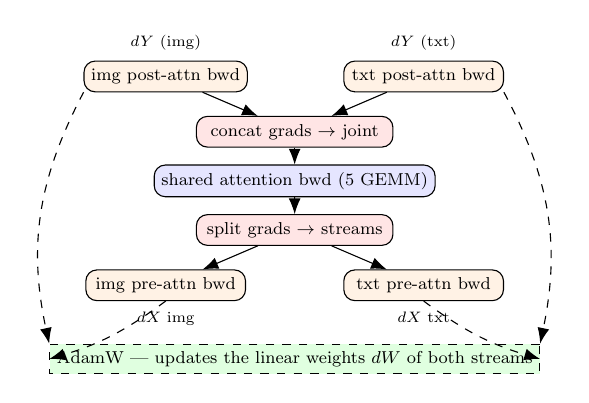
\begin{tikzpicture}[scale=0.78, transform shape, font=\footnotesize, >={Latex[length=2mm]},
  vec/.style={draw, rounded corners, minimum width=2.6cm, minimum height=0.5cm, align=center, fill=orange!10},
  mat/.style={draw, rounded corners, minimum width=2.6cm, minimum height=0.5cm, align=center, fill=blue!10},
  joint/.style={draw, rounded corners, minimum width=3.2cm, minimum height=0.5cm, align=center, fill=red!10}]
\node[vec] (ipost) at (-2.1,2.7) {img post-attn bwd};
\node[vec] (tpost) at (2.1,2.7) {txt post-attn bwd};
\node[joint] (cat) at (0,1.8) {concat grads $\to$ joint};
\node[mat] (attn) at (0,1.0) {shared attention bwd (5 GEMM)};
\node[joint] (split) at (0,0.2) {split grads $\to$ streams};
\node[vec] (ipre) at (-2.1,-0.7) {img pre-attn bwd};
\node[vec] (tpre) at (2.1,-0.7) {txt pre-attn bwd};
\draw[->] (ipost)--(cat); \draw[->] (tpost)--(cat);
\draw[->] (cat)--(attn); \draw[->] (attn)--(split);
\draw[->] (split)--(ipre); \draw[->] (split)--(tpre);
\node[above=0.5mm of ipost] {\scriptsize $dY$ (img)}; \node[above=0.5mm of tpost] {\scriptsize $dY$ (txt)};
\node[below=0.5mm of ipre] {\scriptsize $dX$ img}; \node[below=0.5mm of tpre] {\scriptsize $dX$ txt};
% AdamW consumes the dW of the linears inside ALL four pre/post-attn paths
% of BOTH streams (NOT attention -- attention has no weights).
\node[draw, dashed, fill=green!12, align=center] (adam) at (0,-1.9) {AdamW --- updates the linear weights $dW$ of both streams};
\draw[->,dashed] (ipost.south west) to[bend right=20] (adam.north west);
\draw[->,dashed] (tpost.south east) to[bend left=20] (adam.north east);
\draw[->,dashed] (ipre.south) to[bend left=10] (adam.west);
\draw[->,dashed] (tpre.south) to[bend right=10] (adam.east);
\end{tikzpicture}
\caption{Backward (training) data-flow of the double-stream block. It reuses
the single-stream block's kernels --- including the \emph{same} shared
attention backward (the reverse of the forward's one joint flash attention,
not a DSB-specific kernel) --- run once per stream. The only additions over
the SSB are the concat/split of gradients into and out of the joint sequence;
AdamW updates every weight of both streams.}
\label{fig:dsb-bwd}
\end{figure}

\paragraph{Cost.} Because the double-stream block runs the per-stream
kernels twice but over shorter sequences (the image and text streams are
each a fraction of the joint length) and shares one attention, its total
per-block cost works out close to the single-stream block's --- about
$2.96$\,TFLOP forward, and again roughly $2.2\times$ that for the backward.
The two block types therefore have essentially the same per-block cost
profile; the difference between them is topological, not arithmetic, which
is why an optimisation that helps one helps the other.

\section{Low-precision number formats for inference}
\label{sec:quant}

\subsection{Why precision matters for cost}

Every number the model computes with is stored in some number of bits. The
default for training is 32-bit floating point (FP32), which is accurate but
expensive: it moves a lot of bytes and burns a lot of energy per
operation. Running the model in fewer bits --- \textbf{quantisation} ---
makes each operation cheaper and each memory transfer smaller. The
challenge is doing so without the output visibly degrading.

Because inference runs the backbone tens of times per generation and is
what users pay for, it is the natural place to spend a low-precision
budget. Training, run once and needing numerical robustness, stays at high
precision.

\subsection{FP8 and the MX-E4M3 format}

The low-precision format used here is \textbf{FP8} --- an 8-bit floating
point number --- in the specific \textbf{MX-E4M3} variant. ``E4M3'' means
each 8-bit number has a 4-bit exponent and a 3-bit mantissa, giving it a
wide dynamic range but only coarse precision. On its own, 8 bits is too
coarse for neural-network tensors, so the \textbf{MX} (microscaling)
scheme~\cite{ocp2023mx} adds a shared scale factor for each small block of
values: a group of
elements is stored as 8-bit values plus one E8M0 (8-bit, exponent-only)
\emph{block scale}, so the group can collectively cover whatever magnitude
range it needs. This gives most of the cheapness of 8-bit storage while
recovering much of the accuracy that a flat 8-bit format would lose.

\subsection{Accumulation precision: the key subtlety}

A matrix multiply multiplies many 8-bit numbers and \emph{sums} the
products. Even when the inputs are FP8, that running sum is kept in a wider
format (FP16 or FP32) so the accumulation does not lose precision --- only
the inputs and the final stored result are 8-bit. This distinction matters
for the power model in Chapter~\ref{ch:analysis}: the matrix-multiply
hardware's energy is set by the \emph{accumulation} width (FP8 inputs that
accumulate in FP16 cost the same as an FP16 multiply --- they are not
cheaper on the multiplier), whereas the vector unit and the on-chip and
off-chip memories scale with the \emph{element} bit-width (an 8-bit element
is half the bytes and roughly half the energy of a 16-bit one). The result
is that low-precision inference is the low-energy operating point and
high-precision training is the high-energy one, at \emph{identical} cycle
counts --- precision changes energy, not latency. Section~\ref{sec:quant}
here sets up the formats; Chapter~\ref{ch:analysis} turns them into the
two-leg power model used throughout the results.

\subsection{Calibrating without retraining}

A model trained in FP32 will not, in general, run perfectly in FP8 if
simply truncated, because the most extreme values --- long-tail attention
scores and MLP activations --- are the most sensitive to coarse rounding,
the same activation-outlier problem that motivates post-training methods such
as SmoothQuant~\cite{xiao2023smoothquant} in the LLM setting.
Two standard remedies bridge the gap, both of which reuse the training
machinery rather than introducing anything new: \textbf{post-training
calibration} (collect activation statistics on a small calibration set and
choose good per-block MX scales, with no weight update), and
\textbf{quantisation-aware fine-tuning} (a short run of the normal training
loop with the FP8 quantiser simulated in the forward pass, so the weights
learn to tolerate it). Both are bounded, short stages built from the same
backward and optimiser kernels as full training. As Chapter~\ref{ch:results}
shows, the Open-Sora MMDiT in fact runs in FP8 with no fine-tuning at all
to a cosine of $0.9994$ against the FP32 reference, so for this model
calibration is a safety margin rather than a necessity.

\section{The PLENA accelerator}
\label{sec:plena}

PLENA is the hardware target of this project: a dedicated
\textbf{systolic-array accelerator} for the dense matrix and vector work
that a transformer is made of. Where a GPU is a general-purpose massively
parallel processor, an accelerator like PLENA is specialised --- it does
fewer things, but does the operations a transformer needs with much less
overhead per operation, which is the source of its energy advantage.

% FIGURE TODO fig:plena-arch --- to be supplied by the author:
%   block diagram of one PLENA device (systolic array, vector unit,
%   FPRAM/VRAM/MRAM SRAMs, HBM, instruction/control path).
\begin{figure}[t]
\centering
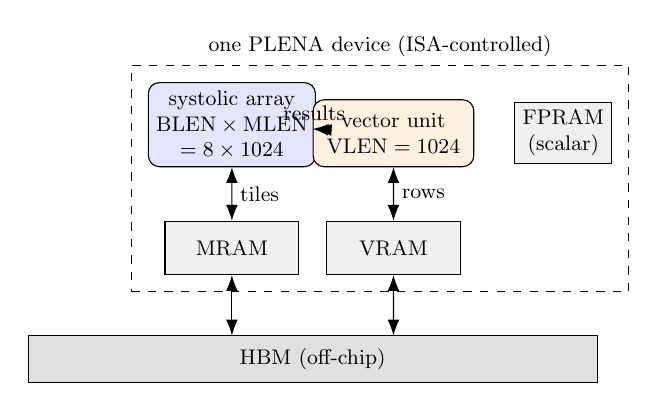
\begin{tikzpicture}[scale=0.85, transform shape, 
  font=\small,
  unit/.style={draw, rounded corners, minimum width=2.4cm, minimum height=1.0cm, align=center},
  sram/.style={draw, fill=black!6, minimum width=2.0cm, minimum height=0.8cm, align=center},
  hbm/.style={draw, fill=black!12, minimum width=8.5cm, minimum height=0.7cm, align=center},
  >={Latex[length=2mm]}]
\node[hbm] (hbm) at (0,0) {HBM (off-chip)};
\node[sram, above left=0.9cm and 0.2cm of hbm.north] (mram) {MRAM};
\node[sram, above right=0.9cm and 0.2cm of hbm.north] (vram) {VRAM};
\node[unit, above=0.8cm of mram, fill=blue!10] (mcu) {systolic array\\$\text{BLEN}\times\text{MLEN}$\\$=8\times1024$};
\node[unit, above=0.8cm of vram, fill=orange!12] (vec) {vector unit\\$\text{VLEN}=1024$};
\node[sram, right=0.6cm of vec, minimum width=1.3cm] (fpram) {FPRAM\\(scalar)};
\draw[<->] (hbm.north -| mram) -- (mram);
\draw[<->] (hbm.north -| vram) -- (vram);
\draw[<->] (mram) -- (mcu) node[midway,right]{tiles};
\draw[<->] (vram) -- (vec) node[midway,right]{rows};
\draw[<->] (mcu) -- (vec) node[midway,above]{results};
\node[draw, dashed, fit=(mcu)(vec)(fpram)(mram)(vram), inner sep=6pt, label=above:{one PLENA device (ISA-controlled)}] {};
\end{tikzpicture}
\caption{Architecture of one PLENA device: the $\text{BLEN}\times\text{MLEN}$
systolic matrix core fed from MRAM, the VLEN-wide vector unit fed from VRAM,
the scalar FPRAM, and the off-chip HBM, all driven by one ISA stream.}
\label{fig:plena-arch}
\end{figure}

\subsection{The matrix core}

The heart of PLENA is a \textbf{systolic array}: a two-dimensional grid of
$\text{BLEN} \times \text{MLEN}$ small multiply-accumulate (MAC) units that
streams a matrix through itself, with each cell multiplying a pair of
inputs and adding to a running sum. The systolic array is a long-established
dataflow for dense linear algebra and the basis of production deep-learning
accelerators such as Google's TPU~\cite{jouppi2017tpu}; PLENA applies the same
principle to the MMDiT. A systolic array is extremely
efficient on exactly the operation a transformer spends most of its time
on --- large dense GEMMs and attention --- because data flows directly
between neighbouring cells with almost no instruction or memory overhead.
At the dimensions used here the array is $\text{BLEN}=8$ wide and
$\text{MLEN}=1024$, so one device performs many thousands of MACs per
cycle. The array's \emph{cycle count} for a given matrix is fixed by these
dimensions and the operation's size --- and, importantly, is the same
whether the data is FP8 or FP32. Only the energy per cycle changes with
precision.

\subsection{The vector unit}

Not everything is a matrix multiply. Normalisation, modulation, GELU, the
softmax inside attention, RoPE rotations, and the AdamW update are all
\textbf{element-wise or per-row} operations. PLENA handles these on a
separate \textbf{vector unit} of width $\text{VLEN}=1024$, which applies
the same operation across a whole row of elements at once. Some of these
operations are awkward on the hardware --- for example there is no vector
square-root instruction, so normalisation computes a reciprocal
square-root with a short Newton--Raphson iteration --- and these details
are dealt with at the kernel level in Chapter~\ref{ch:implementation}.

\subsection{The memory hierarchy}

Data lives at several levels, fastest and smallest first: small on-chip
register and scratch memories feed the matrix and vector units directly; a
larger on-chip \textbf{SRAM} (split into a matrix-side and a vector-side
store) holds the tiles currently being worked on; and a large off-chip
\textbf{HBM} (high-bandwidth memory) holds the full weights and
activations. A central concern when mapping a model is keeping the matrix
core fed: if data cannot be staged from HBM through SRAM into the array
fast enough, the array stalls. For the Open-Sora blocks this turns out not
to be the bottleneck --- the workload is firmly \emph{compute-bound}, with
the matrix core, not the memory, as the limiting resource ---
which is what makes a matrix accelerator the right choice for it.

\subsection{The instruction set and multi-device execution}

PLENA is programmed through a custom \textbf{instruction set (ISA)}: matrix
instructions that drive the systolic array, vector instructions for the
element-wise work, and load/store and control instructions that move data
and manage loops. Our kernels are ultimately expressed as sequences of
these instructions, and Chapter~\ref{ch:implementation} measures latency
and energy by analysing exactly the compiled instruction stream.

Finally, one PLENA device is small relative to a whole MMDiT block, so work
is spread across \textbf{many devices in parallel}. The model is naturally
parallel --- a block applies the same computation across many tokens and
attention heads --- so a single kernel is split across a set of devices,
with each device handling a slice of the work and the remainder folded into
a loop when there are more slices than devices. Chapter~\ref{ch:analysis}
sizes this device count so that the PLENA system is matched to one NVIDIA
A100's compute budget on the same process node, which is the basis for
every latency and energy comparison in the report.

\section{The compilation flow}
\label{sec:compiler}

The kernels in this report are not written directly as PLENA instructions.
They are written in an ordinary, high-level GPU-style form using
\textbf{TileLang} --- the same way one would write a kernel for a GPU ---
and a \textbf{compiler} lowers that high-level description down to the
PLENA ISA. This compiler is itself a significant part of the wider project,
but it is a \emph{tool} this report uses rather than its subject, so this
section describes only its core function and the two ideas that make it
effective; it is not a pass-by-pass account.

\subsection{The core problem: a SIMT language on a SIMD machine}

TileLang is normally compiled for NVIDIA GPUs, whose execution model is
\textbf{SIMT} (single-instruction, multiple-thread): many independent
threads, each with its own program counter, grouped into warps and blocks.
PLENA is instead a \textbf{SIMD} (single-instruction, multiple-data)
machine: one instruction stream drives wide vector and tile datapaths,
with no per-thread divergence. The central job of the compiler is to take a
program written in the GPU-flavoured SIMT style and map it efficiently onto
PLENA's SIMD units, \emph{without} requiring the author to learn a new
language. The payoff of preserving the familiar style is real: SIMT kernels
are far easier to write --- and to optimise --- than hand-written SIMD, so
keeping that front-end is a feature, not a compromise. Concretely, the
compiler maps TileLang's GPU memory scopes onto PLENA's storage units
(shared memory onto the matrix and vector SRAMs, fragments onto the vector
or scalar RAMs), so the usual global-to-shared GPU idioms carry over
unchanged.

\subsection{The frontend: block fusion}

The compiler's most important optimisation is \textbf{block fusion}:
merging adjacent operations of a kernel so that the hardware does less
redundant work. It takes two complementary forms.

\begin{itemize}
\item \textbf{Memory-access fusion.} A naive lowering moves a tensor out to
memory after each operation and reads it back for the next. Because the
transformer blocks here are long chains of operations over the same tiles,
that round-tripping dominates. Block fusion merges these accesses ---
keeping a tile resident and combining its loads and stores --- so the
memory system is touched once for a run of operations instead of once per
operation. On a compute-bound workload this is what keeps the memory path
off the critical path.
\item \textbf{Compute fusion.} Where consecutive arithmetic operations act
on data already in the datapath, the compiler fuses them into a single
pass rather than emitting, and re-reading, an intermediate result for each.
This keeps values in registers and the vector unit across an operation
chain (for example a normalise--modulate--activation sequence), cutting
both the instruction count and the traffic to on-chip memory.
\end{itemize}

Together these two fusions are what let generated code beat a hand-written
baseline: the author writes each operation plainly, and the compiler
removes the boundaries between them.

\subsection{The backend: an LLVM-style optimiser}

After fusion, the kernel still contains a great deal of integer
\emph{address arithmetic} --- the index computations that locate each tile
in memory, generated mechanically and full of redundancy. The backend
lowers this to a low-level, register-based intermediate representation in
the spirit of \textbf{LLVM}, in \textbf{static single-assignment (SSA)}
form, and runs the same classical scalar optimisations a general-purpose
compiler would: \textbf{constant folding}, \textbf{dead-code elimination},
\textbf{common-subexpression elimination (CSE)}, \textbf{reassociation},
and \textbf{loop-invariant code motion (LICM)} to hoist address
computations out of inner loops. These run to a fixed point before the
final stage assigns physical registers and emits the \texttt{.isa} text.
The effect is large: the bulk of a transformer kernel's non-matrix
instructions are address arithmetic, and treating it with a real
optimising backend --- rather than emitting it verbatim --- is what makes
the compiled instruction stream tight enough to be competitive.

\medskip
The only facts the rest of the report depends on are these: kernels are
authored once in high-level TileLang; block fusion merges their memory
accesses and compute; and an LLVM-style backend optimises the resulting
address arithmetic before emitting the exact ISA stream that the latency
and energy analysis in Chapters~\ref{ch:implementation}--\ref{ch:results}
is measured on.


% #####################################################################
% CHAPTER 3 — ANALYSIS AND DESIGN
% #####################################################################
\chapter{Analysis and Design}
\label{ch:analysis}

Chapter~\ref{ch:background} established \emph{what} the MMDiT computes.
This chapter fixes the design decisions that turn it into a measurable
acceleration study. It begins by pinning down the model's exact dimensions
(Section~\ref{sec:model-shape}), since every later number --- compute
counts, memory layout, device geometry --- is derived from them. It then
identifies which kernels are worth targeting
(Section~\ref{sec:targets}), at what numerical precision each phase runs
and how precision scales energy (Section~\ref{sec:precision-design}), what
hardware the result is compared against (Section~\ref{sec:a100-match}), how
the per-device geometry and compute balance are chosen
(Sections~\ref{sec:mem-angle}--\ref{sec:compute-angle}), and how a single
block is spread across many devices (Section~\ref{sec:device-alloc}).
Together these define the experimental setup measured in
Chapter~\ref{ch:results}.

\section{Model shape}
\label{sec:model-shape}

Almost everything in this chapter --- the FLOP counts, the memory layout,
the choice of device geometry --- follows arithmetically from a handful of
model dimensions. We therefore state them once, here, and refer back to
them throughout. The numbers are Open-Sora's real values; where the true
sizes are not a multiple of the hardware lane width they are padded up, and
both the real and padded figures are given.

\subsection{The dimensions that matter}

A single MMDiT pass operates on a \textbf{sequence of tokens}, each of which
is a vector of \textbf{hidden width} $\text{HD}$. The hidden width is itself
a stack of attention \textbf{heads}: $\text{HEAD}$ heads, each of dimension
$\text{HLEN}$, so $\text{HD}=\text{HEAD}\times\text{HLEN}$. Inside the MLP,
each token is temporarily widened by an $\text{mlp\_ratio}$ factor. The
concrete values are:

\begin{table}[h]
\centering
\caption{Open-Sora model dimensions used throughout this report. Padded
values round the true size up to a multiple of the hardware lane width
$\text{MLEN}=1024$; the difference is masked out and does not affect
correctness.}
\label{tab:model-shape}
\begin{tabular}{@{}llr@{}}
\toprule
Symbol & Meaning & Value \\
\midrule
$\text{HLEN}$ & head dimension & 128 \\
$\text{HEAD}$ & number of attention heads & 24 \\
$\text{HD}$ & hidden width $=\text{HEAD}\cdot\text{HLEN}$ & 3072 \\
$\text{mlp\_ratio}$ & MLP widening factor & 4 \\
$\text{MHD}$ & MLP hidden width $=4\,\text{HD}$ & 12288 \\
$5\,\text{HD}$ & fused proj+MLP-out contraction $=\text{HD}+\text{MHD}$ & 15360 \\
\midrule
\multicolumn{3}{@{}l}{\emph{Sequence lengths (real $\to$ padded to a multiple of 1024):}}\\
$S_{\text{SSB}}$ & single-stream joint sequence & $8828 \to 9216$ \\
$S_{\text{img}}$ & double-stream image stream & $8316 \to 9216$ \\
$S_{\text{txt}}$ & double-stream text stream & $512 \to 1024$ \\
$S_{\text{joint}}$ & double-stream concatenated sequence & $10240$ \\
\bottomrule
\end{tabular}
\end{table}

\subsection{Why these two numbers dominate everything}

Two of these dimensions deserve emphasis, because the rest of the chapter
turns on them:

\begin{itemize}
\item \textbf{The sequence length $S \approx 9216$ is what makes the model
expensive.} The dense linear layers cost grows \emph{linearly} in $S$, but
attention grows with $S^2$ --- every token attends to every other. At
roughly nine thousand tokens the $S^2$ term is enormous, which is why
attention is the single heaviest kernel (Section~\ref{sec:targets}) and why
its mixed matrix/vector profile dominates the compute-balance analysis
(Section~\ref{sec:compute-angle}). A long sequence is the defining feature
of a video MMDiT and the root cause of its cost.
\item \textbf{The head dimension $\text{HLEN}=128$ is what dictates the
hardware layout.} As Section~\ref{sec:mem-angle} shows, the on-chip memory
must pack whole $128$-wide heads into its lanes without padding, which forces
the device width to be a multiple of $128$ --- and ultimately fixes
$\text{MLEN}=\text{VLEN}=1024$. The head dimension is the bridge between the
model and the machine.
\end{itemize}

With these dimensions fixed, the FLOP counts, the memory layout, and the
device geometry in the rest of the chapter all follow as arithmetic.

\section{Where the compute is, and what to target}
\label{sec:targets}

The whole-model breakdown in Section~\ref{sec:compute-breakdown} already
settled the first design question. Across a full generation the MMDiT
forward pass is \textbf{99.4\%} of the arithmetic; the VAE decode and the
text encoders together are under $0.6\%$. Accelerating Open-Sora is thus,
to within rounding, accelerating the MMDiT --- so the VAE and encoders are
deliberately left out of scope, and all hardware effort goes to the
backbone.

Zooming one level in, the per-block analysis of Section~\ref{sec:blocks}
settled the second. Within one MMDiT pass the single- and double-stream
blocks are $99.8\%$ of the work, split roughly two-thirds to the
single-stream block and one-third to the double-stream block, with the tiny
output head negligible. And within a block, Tables~\ref{tab:fwd-kernels}
and~\ref{tab:bwd-kernels} showed that the \textbf{matrix kernels} --- the
linear layers and attention --- carry essentially all of the FLOPs, while
the seven vector kernels are a few percent combined. The design conclusion
is therefore sharp:

\begin{itemize}
\item \textbf{Target the two block types}, not the model scaffolding. The
same kernel set serves both, so the implementation effort is shared.
\item \textbf{Optimise for the matrix kernels.} The accelerator must keep
its systolic array busy on the linear layers and attention; the vector
kernels must merely keep up without stalling it.
\item \textbf{Both phases matter.} Inference (forward only) is the
latency-critical path run tens of times per generation; training (forward
+ backward + optimiser) is ${\sim}3\times$ the per-step matrix work and is
the high-cost end of the study. Both are implemented and measured.
\end{itemize}

\section{Precision design: low-precision inference, high-precision training}
\label{sec:precision-design}

\subsection{The two operating points}

The two phases run at two different numerical precisions, for the reasons
introduced in Section~\ref{sec:quant}:

\begin{itemize}
\item \textbf{Inference $\to$ MX-E4M3 (low precision).} The denoising loop
runs the backbone ${\sim}150$ times per generation and is what users pay
for, so it runs at the cheapest viable format. All HBM tensors are stored
in MX-E4M3 (8-bit element plus an E8M0 block scale). This is the
low-energy operating point.
\item \textbf{Training $\to$ FP32 (high precision).} Gradients span a wide
dynamic range and low-precision accumulation degrades convergence, so the
backward pass and the optimiser keep full 32-bit floating point. This is
the high-energy operating point.
\end{itemize}

\subsection{What precision changes --- and what it does not}

The key modelling fact is that \textbf{precision is cycle-invariant but not
energy-invariant}. The number of cycles a kernel takes is fixed by the
systolic-array geometry ($\text{BLEN}\times\text{MLEN}$) and the operation
size: an FP32 GEMM and an FP8 GEMM of the same shape take the \emph{same}
number of cycles, so \textbf{latency does not depend on precision}. What
changes is the energy per cycle, and it does so along \textbf{two separate
legs}, anchored to an FP16 baseline (MAC $=1$\,mW, vector lane $=0.5$\,mW,
SRAM $=0.055$\,pJ/bit):

\begin{itemize}
\item \textbf{The matrix core scales with \emph{accumulation} precision.}
FP8 inputs accumulate into FP16, so the MAC array stays at the FP16 energy
level --- FP8 matrix work is $1\times$, \emph{not} halved; only FP32
accumulation doubles it to $2\times$.
\item \textbf{The vector unit and the SRAMs scale with \emph{element}
bit-width.} An 8-bit element is half the bytes and roughly half the energy
of a 16-bit one: FP8 $=0.5\times$, FP16 $=1\times$, FP32 $=2\times$. The
HBM byte count tracks the same factor and scales memory time.
\end{itemize}

\begin{table}[t]
\centering
\caption{The two-leg precision scaling, relative to the FP16 baseline. The
matrix (MCU) leg follows accumulation precision; the vector/SRAM/HBM leg
follows element bit-width. Cycle count --- and therefore latency --- is
unchanged across all rows.}
\label{tab:precision}
\begin{tabular}{@{}lccc@{}}
\toprule
Phase / format & MCU (matmul) & Vector + SRAM + HBM & Latency \\
\midrule
Inference --- MX-E4M3 / FP8 & $1\times$ & $0.5\times$ & unchanged \\
(FP16 baseline) & $1\times$ & $1\times$ & unchanged \\
Training --- FP32 & $2\times$ & $2\times$ & unchanged \\
\bottomrule
\end{tabular}
\end{table}

Table~\ref{tab:precision} summarises the scaling. The consequence is that
inference sits at the low-energy corner (matrix $1\times$, vector/memory
$0.5\times$) and training at the high-energy corner (everything $2\times$),
at \emph{identical} cycle counts. Precision is therefore modelled as an
explicit, first-class knob in the energy tool rather than baked in, which
is what lets Chapter~\ref{ch:results} report inference and training energy
from the same compiled kernels.

\section{Sizing the hardware}
\label{sec:hw-sizing}

Fixing the PLENA configuration --- the shape of one device and how many of
them to deploy --- is the central hardware-design decision of the project.
The shape of a single device is settled by a \textbf{memory angle}
(Section~\ref{sec:mem-angle}): the on-chip geometry must let a block's
tensors be laid out and streamed at the highest possible bandwidth
\emph{without padding}, because any padded lane is bandwidth and energy
spent moving zeros. This pins the per-device geometry to
$\text{MLEN}=\text{VLEN}=1024$.

Separately, the experiment needs a fair baseline: the total PLENA hardware
must be of comparable size to the A100 it is measured against
(Section~\ref{sec:a100-match}), which fixes how many devices are deployed.
On top of these two --- a fixed device shape and a fixed device budget ---
sits the \textbf{compute angle} (Section~\ref{sec:compute-angle}), which
decides how the work itself is shaped and distributed across that hardware.

\section{The memory angle: head layout and the no-padding geometry}
\label{sec:mem-angle}

\subsection{Why padding is the enemy}

A PLENA device moves data in fixed-width lanes: the matrix and vector
datapaths are $\text{MLEN}=\text{VLEN}=1024$ elements wide, and a transfer
either fills those lanes or wastes the unused ones. If a tensor's natural
shape does not tile evenly onto the lane width, the spare lanes must be
\emph{padded} with zeros --- and those zeros are loaded, stored, and
computed on exactly as if they were data. Padding therefore costs real
bandwidth and real energy while contributing nothing. The first design
goal is consequently \textbf{maximum effective bandwidth with zero
padding}: every lane of every transfer should carry a useful element.

For a transformer the quantity that must tile cleanly is the
\textbf{attention head}. The model's hidden width is a stack of $\text{HEAD}$
heads each of width $\text{HLEN}$ (head dimension); at Open-Sora's
dimensions $\text{HEAD}=24$ and $\text{HLEN}=128$, so the hidden width is
$\text{HD}=\text{HEAD}\cdot\text{HLEN}=3072$. The question the memory
angle must answer is: \emph{how should these heads be arranged across the
on-chip memories so that a head-structured tensor fills the lanes exactly?}

\subsection{How heads are laid out in MRAM and VRAM}

PLENA stores a head-structured tensor by \textbf{packing several heads
side by side across the lane width}. The lane dimension of width $1024$ is
divided into $\text{lane\_count}$ slots, each $\text{HLEN}=128$ elements
wide, so that $\text{lane\_count}$ whole heads sit next to one another in
one lane-width transfer. With a head dimension of $128$, a $1024$-wide
datapath holds
\[
\text{lane\_count} = \frac{\text{MLEN}}{\text{HLEN}} = \frac{1024}{128} = 8
\]
heads at once. The remaining heads (here $24/8 = 3$ groups of eight) are
stacked along the orthogonal, row direction. The same packing applies on
both sides of the on-chip memory, with the two memories playing
complementary roles in a matrix multiply: the \textbf{MRAM} (matrix RAM)
holds the operand that streams \emph{stationary} into the systolic array,
and the \textbf{VRAM} (vector RAM) holds the operand and results that the
vector unit reads and writes per row. Laying the heads out identically in
both --- eight packed across the lanes, the rest stacked down the rows ---
is what lets attention and the linear layers hand tensors back and forth
between the matrix core and the vector unit without ever re-shuffling them.

% FIGURE TODO fig:head-layout --- to be drawn:
%   show the 1024-wide lane dimension split into 8 slots of HLEN=128
%   (8 heads packed across lanes), the remaining head-groups stacked
%   down the rows, mirrored in MRAM (stationary matrix operand) and
%   VRAM (vector operand/result). Annotate lane_count=8, HLEN=128,
%   MLEN=VLEN=1024, and the "no padding" fit.
\begin{figure}[t]
\centering
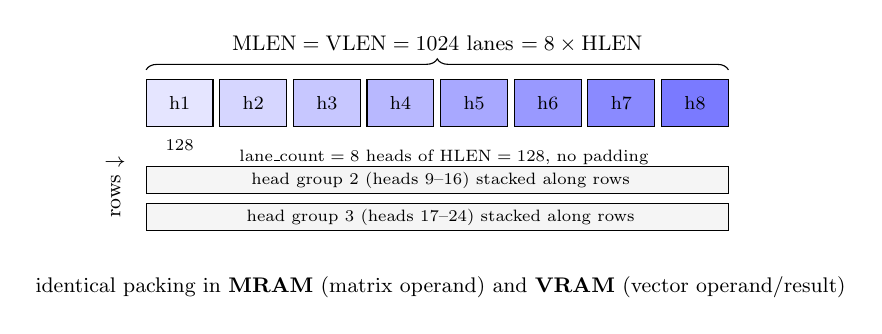
\begin{tikzpicture}[scale=0.85, transform shape, font=\small, >={Latex[length=2mm]}]
% 8 head slots across the 1024-wide lane dimension
\foreach \i in {0,...,7}{
  \fill[blue!\the\numexpr10+\i*6\relax] (\i*1.1,0) rectangle ++(1.0,0.7);
  \draw (\i*1.1,0) rectangle ++(1.0,0.7);
  \node at (\i*1.1+0.5,0.35) {\footnotesize h\the\numexpr\i+1\relax};
}
% lane-width brace
\draw[decorate,decoration={brace,amplitude=4pt}] (0,0.85) -- (8*1.1-0.1,0.85)
  node[midway,above=4pt]{$\text{MLEN}=\text{VLEN}=1024$ lanes $=8\times\text{HLEN}$};
\node[below=2pt] at (0.5,0) {\scriptsize 128};
\node[below=2pt] at (4.45,-0.15) {\scriptsize $\text{lane\_count}=8$ heads of $\text{HLEN}=128$, no padding};
% row stacking: further head groups stacked downward
\foreach \r in {1,2}{
  \draw[fill=black!4] (0,-\r*0.55-0.45) rectangle ++(8*1.1-0.1,0.4);
  \node at (4.4,-\r*0.55-0.25) {\scriptsize head group \the\numexpr\r+1\relax\ (heads \the\numexpr\r*8+1\relax--\the\numexpr\r*8+8\relax) stacked along rows};
}
\node[left=0.2cm of {(0,-0.9)}, rotate=90, anchor=south] {rows $\downarrow$};
% mirrored in MRAM/VRAM note
\node[align=center] at (4.4,-2.4) {identical packing in \textbf{MRAM} (matrix operand) and \textbf{VRAM} (vector operand/result)};
\end{tikzpicture}
\caption{Head layout across MRAM and VRAM. Eight heads of width
$\text{HLEN}=128$ pack exactly into the $\text{MLEN}=\text{VLEN}=1024$ lane
width ($\text{lane\_count}=8$), with no padding; the remaining heads
($24/8=3$ groups in total) stack along the row direction. The same packing
is mirrored in both memories, so tensors pass between the matrix core and the
vector unit with no re-shuffling.}
\label{fig:head-layout}
\end{figure}

\subsection{The optimal geometry: $\text{MLEN}=\text{VLEN}=\text{lane\_count}\times\text{HLEN}=1024$}

This layout is only padding-free when the lane width is an exact multiple
of the head dimension. That single requirement fixes the whole per-device
geometry. Reading it off the layout:

\[
\boxed{\;\text{MLEN} \;=\; \text{VLEN} \;=\; \text{lane\_count} \times \text{HLEN} \;=\; 8 \times 128 \;=\; 1024.\;}
\]

Each term is forced for a concrete reason:

\begin{itemize}
\item \textbf{$\text{HLEN}=128$} is the model's head dimension --- given, not
chosen.
\item \textbf{$\text{MLEN}=\text{VLEN}$.} The matrix datapath and the vector
datapath must be the \emph{same} width, or every tensor handed from the
matrix core to the vector unit (and back) would need re-tiling; equal
widths make the hand-off a no-op, which matters because every block
alternates matrix and vector kernels.
\item \textbf{$\text{lane\_count}=8$.} Packing $\text{MLEN}/\text{HLEN}=8$
heads across the lanes is the largest whole number of heads that fits a
$1024$-wide datapath exactly. Choosing a width that was not a multiple of
$128$ would strand a partial head in the spare lanes and force padding;
$8\times128=1024$ fits perfectly.
\item \textbf{$1024$} is therefore the smallest lane width that packs a
whole number of $128$-wide heads \emph{and} keeps the two datapaths equal.
A wider datapath would only help if it stayed a multiple of $128$ and the
extra lanes were always filled --- otherwise it reintroduces padding.
\end{itemize}

In short, the memory angle does not leave the device shape free: requiring a
padding-free head layout with matched matrix and vector widths forces
$\text{MLEN}=\text{VLEN}=1024$ and $\text{lane\_count}=8$ at the model's
$\text{HLEN}=128$. This is the per-device shape used everywhere in the
report. (The same relation also sets the broadcast amount used by the
modulation and norm kernels, $\text{broadcast}=\text{MLEN}/\text{HLEN}=8$,
which is why these geometry terms are always derived from the head
dimension rather than hard-coded.) What the memory angle leaves open is
\emph{how many} such devices to deploy --- which is fixed later, by the
comparison budget of Section~\ref{sec:a100-match}.

\subsection{Consequence: a wide, padding-free device does not hit the memory wall}

The payoff of this geometry is bandwidth. Because every lane of every
transfer carries a useful head element --- no zeros are moved and no lane
is wasted --- a single device's \emph{effective} memory bandwidth is close
to its peak, not the fraction left after padding. A device that can stage
operands into the systolic array this efficiently is rarely starved: the
matrix core is fed fast enough that it, not the memory path, is the
limiting resource. In other words, the no-padding head layout is what keeps
the MMDiT workload firmly \textbf{compute-bound} on PLENA rather than
\emph{memory-bound} --- it does not hit the ``memory wall'' where a kernel
spends most of its time waiting on data movement. This is the design-side
reason behind the compute-bound behaviour already noted for the memory
hierarchy in Section~\ref{sec:plena}, and it is precisely the regime in
which a matrix accelerator is the right tool: if the workload were
memory-bound, a bigger systolic array would buy nothing, but because it is
compute-bound, adding matrix throughput --- by deploying more devices,
fixed later in Section~\ref{sec:a100-match} --- translates directly into
speed.

\section{The compute angle: compute balance}
\label{sec:compute-angle}

The memory angle fixed the shape of a device; the compute angle is about how
well that hardware is actually \emph{used}, and it is what fixes the
\emph{internal} throughput split that a balanced device needs (how much
matrix versus vector versus scalar capability to provision). Its central
concept is \textbf{compute balance}, and it is what ties the design directly
to latency. With the device shape and its internal balance both settled, the
remaining question --- how many devices to deploy --- is then fixed by the
comparison budget in Section~\ref{sec:a100-match}.

\subsection{The barrel principle}

A PLENA device is not one engine but three that run \textbf{in series, with
no overlap}: the \textbf{matrix} unit (the systolic array), the
\textbf{vector} unit, and the \textbf{scalar} unit. A kernel that needs all
three runs its matrix work, then its vector work, then its scalar work ---
they do not execute concurrently. The latency of a kernel is therefore the
\emph{sum} of the time each unit is busy, and the latency of a block is the
sum over its kernels.

This makes throughput allocation inside a device behave like a barrel made
of staves of different heights: the amount of water it holds is set by the
\emph{shortest} stave, not the average. If the matrix unit is enormously
powerful but the vector unit is weak, then any kernel with a non-trivial
vector phase stalls waiting on the vector unit, and the matrix unit's power
is wasted for that stretch. Balancing the per-cycle throughput of the
matrix, vector, and scalar units against the \emph{mix of work the model
actually presents} is therefore the key compute-side design decision: a
device tuned for one kernel can be badly mismatched to another.

To decide that balance we need to know, kernel by kernel, how much of each
kind of work the block contains.

\subsection{Per-kernel compute breakdown}

Table~\ref{tab:compute-balance} gives a pure-FLOP analysis of \textbf{one
full MMDiT forward pass} --- all 38 single-stream blocks, all 19
double-stream blocks, and the final output layer --- at the Open-Sora
dimensions of Table~\ref{tab:model-shape}. This is the quantity introduced
in Section~\ref{sec:compute-breakdown} ($168.9$\,TFLOP per pass); here we
break it down by kernel class so the device can be balanced against the
real mix of work. (The backward pass, used only in training, was analysed
separately in Section~\ref{sec:bwd-kernels}; here we size the device for the
latency-critical forward path.)

Each kernel class's work is split into the part that lands on the matrix
unit (dense GEMMs) and the part that lands on the vector unit (element-wise
and per-row operations, including the attention softmax). Every matrix
kernel is annotated with its per-block GEMM \textbf{shape}
$m\times k\times n$, from which the FLOP count follows exactly as $2mkn$;
the totals then aggregate that over all 57 blocks. The shapes use the real
sequence length $S=8828$, so the per-block figure is $2.96$\,TFLOP and the
pass total is $168.9$\,TFLOP, matching Section~\ref{sec:compute-breakdown}.
Writing the shapes out makes the source of every number explicit: they are
nothing more than the model dimensions of Table~\ref{tab:model-shape}
substituted in and multiplied by the block counts.

\begin{table}[t]
\centering
\caption{Pure-FLOP compute breakdown of \textbf{one full MMDiT forward pass}
(38 SSB + 19 DSB + final layer) at Open-Sora dimensions, real sequence
$S=8828$. Matrix kernels show their per-block GEMM shape $m\times k\times n$
(FLOP $=2mkn$); attention shapes are per head, over $\text{HEAD}=24$ heads.
The ``Pass total'' column aggregates each kernel class over all 57 blocks.
``Vector'' work (norms, RoPE, GELU, softmax, gates) is well under $1\%$ of
the FLOPs but, as the text explains, not of the time.}
\label{tab:compute-balance}
\begin{tabular}{@{}llrl@{}}
\toprule
Kernel class & Per-block shape ($m{\times}k{\times}n$) & Pass total & Bound \\
 & & (TFLOP) & \\
\midrule
Q / K / V linears ($\times3$) & $8828\times3072\times3072$ & 28.5 & matrix \\
MLP-in linear & $8828\times3072\times12288$ & 38.0 & matrix \\
\textbf{Attention} $QK^\top$ & $24\times(8828{\times}128{\times}8828)$ & 27.3 & matrix \\
\textbf{Attention} softmax & $24\times(8828{\times}8828)$ & vector & vector \\
\textbf{Attention} $PV$ & $24\times(8828{\times}8828{\times}128)$ & 27.3 & matrix \\
Output linear & $8828\times15360\times3072$ & 47.5 & matrix \\
LayerNorm / mod / QK-norm / RoPE / GELU / gate & per-row over the tensor & $<1$ & vector \\
final layer (adaLN + output proj) & --- & 0.34 & matrix \\
\midrule
\textbf{MMDiT forward pass total} & & \textbf{168.9} & matrix-dom. \\
\bottomrule
\end{tabular}
\end{table}

Two readings of this table matter, and they are different:

\begin{itemize}
\item \textbf{By raw FLOP count, the pass is overwhelmingly matrix work.}
The dense linears and the attention GEMMs are the full $168.9$\,TFLOP; the
vector kernels are a fraction of a percent of the FLOPs. A pure-FLOP view
says ``build a big matrix unit and the vector unit barely matters.''
\item \textbf{By time, the picture is less one-sided}, because of the
barrel principle. The vector unit processes far fewer elements per cycle
than the matrix array does MACs per cycle, so a vector kernel takes many
more cycles per FLOP than a matrix kernel. A vector phase that is tiny in
FLOPs can still consume real time --- and since the units do not overlap,
that time adds directly to latency. This is why the vector
unit cannot simply be starved to feed the matrix unit: under-provision it
and the short stave shortens the whole barrel.
\end{itemize}

\subsection{Why attention is the hard case}

Every other kernel is \emph{pure}: the linears are matrix-only, the norms
and RoPE and GELU are vector-only, so each one exercises a single unit and
is easy to reason about. \textbf{Attention is the exception, and it is the
single hardest kernel to balance for three compounding reasons:}

\begin{enumerate}
\item \textbf{It is genuinely mixed.} A single attention kernel contains
both large matrix work --- the $QK^\top$ scores and the $PV$ value mix,
together the biggest matrix term in the pass at $54.6$\,TFLOP ($27.3+27.3$),
about a third of all matrix work --- \emph{and} a substantial vector phase,
the softmax over those scores. No other kernel forces the matrix and vector
units to hand off back and forth within one operation.
\item \textbf{The two phases cannot overlap.} Because the units run in
series, the softmax cannot be hidden behind the GEMMs: the kernel must do
matrix work, then vector work, then more matrix work, paying for each in
full. The softmax operates on all $\text{HEAD}\times S \times S$ scores ---
a number that grows with the \emph{square} of the sequence length --- so at
Open-Sora's $S\approx9216$ this vector phase is far from negligible.
\item \textbf{It dominates the block.} Taken together, attention's matrix
and serial vector phases typically account for around \textbf{half of a
block's wall-clock time}: it is the largest matrix term \emph{and} the only
one carrying a non-trivial, non-overlappable vector phase, so by time --- not
just FLOPs --- it is the heaviest part of the block. It is therefore the
kernel whose balance matters most: a device tuned so that attention runs
without stalling --- enough vector throughput to keep its softmax phase
short relative to its GEMMs --- will run the whole block well, whereas a
device that balances for the pure linears alone will stall badly inside
attention.
\end{enumerate}

Attention is thus the kernel that sets the compute-balance target. The
matrix unit must be sized for its GEMMs (the dominant FLOP term), but the
vector unit must be sized so that attention's softmax does not become the
short stave --- and this trade-off, rather than the raw FLOP majority, is
what the per-device throughput allocation must satisfy.

\subsection{The backward pass}
\label{sec:compute-backward}

The analysis so far is for the forward pass, which is also inference. Training
adds the backward pass, and the device must serve it too, so its compute is
analysed the same way. The defining property is the \emph{one-forward,
two-backward} rule: every forward linear becomes two backward GEMMs (an
input-gradient $dX$ and a weight-gradient $dW$), and attention's backward
expands to five GEMMs (Section~\ref{sec:bwd-kernels}). Substituting the same
model dimensions gives Table~\ref{tab:compute-backward}.

\begin{table}[h]
\centering
\caption{Pure-FLOP compute breakdown of \textbf{one full MMDiT backward pass}
(real sequence $S=8828$, aggregated over all 57 blocks). Each forward linear
becomes two GEMMs ($dX{+}dW$); attention becomes five. The backward is
$2.16\times$ the forward matrix work.}
\label{tab:compute-backward}
\begin{tabular}{@{}llr@{}}
\toprule
Backward kernel class & GEMMs & Pass total (TFLOP) \\
\midrule
Q / K / V linears ($dX{+}dW$, $\times3$) & 6 & 57.0 \\
MLP-in linear ($dX{+}dW$) & 2 & 76.0 \\
Output linear ($dX{+}dW$) & 2 & 95.0 \\
Attention ($dQ,dK,dV$) & 5 & 136.5 \\
Norm / RoPE / GELU / affine backward & --- & $<1$ (vector) \\
\midrule
\textbf{MMDiT backward pass total} & & \textbf{364.4} \\
\textbf{(forward was 168.9)} & & \textbf{$2.16\times$ forward} \\
\bottomrule
\end{tabular}
\end{table}

Two design consequences follow. First, the backward roughly \emph{doubles}
the per-step matrix work, so a training step (forward $+$ backward) is about
three times the matrix cost of an inference pass --- which, combined with the
FP32 precision tier (Section~\ref{sec:precision-design}), makes training the
high-cost end of the workload. Second, the backward is \emph{even more
matrix-bound} than the forward: the extra GEMMs add matrix work without
adding vector work (the attention backward reuses the saved softmax
statistics rather than recomputing the reductions,
Section~\ref{sec:bwd-kernels}), so the compute-balance pressure on the vector
unit is, if anything, lower in the backward than in the forward. The device
sized for the forward's attention balance therefore also serves the backward
without a separate balancing target.

\section{Edge computation: what to offload to the host}
\label{sec:edge}

Not every operation in a forward or backward pass belongs on the
accelerator. PLENA exists to do dense matrix work; some operations are so
\emph{small and irregular} that placing them on it wastes the systolic array
and the on-chip memory, and they are better done on a general-purpose host
(the ``edge'' of the computation). Deciding what to offload is a real design
choice, and the compute analysis makes the cut clear.

\paragraph{The conditioning (adaLN) parameter generation belongs on the
host.} The clearest example is how the modulation parameters are produced.
Each block is conditioned by a single \emph{vector} (the noise-level and
prompt summary), which is expanded --- through a SiLU and a small linear ---
into the per-block \textbf{shift, scale, and gate} parameters that the
modulation and residual-gate kernels consume. This expansion has three
awkward properties: it operates on a single $1\times\text{HD}$ \emph{row}
(not a full $S\times\text{HD}$ tensor), so it cannot fill the matrix array;
it produces a \emph{different} set of parameters for every block and every
denoising step, so there is nothing to amortise; and it is a tiny fraction of
the arithmetic. Running this on the systolic array would occupy it with a
near-empty, one-row computation that changes every iteration. It is therefore
treated as an \textbf{edge computation}: the per-block shift/scale/gate are
generated on the host and supplied to the accelerator alongside the weights,
so PLENA only ever \emph{applies} the modulation (a cheap whole-tensor vector
op) and never spends matrix cycles \emph{computing} it. The same reasoning
applies to other small, per-step, host-side bookkeeping (assembling the vecs,
the sampler's loop control), which never touches the accelerator at all.

\paragraph{The final layer stays on the accelerator --- and is provably
tiny.} Not every small operation is offloaded. The MMDiT \emph{final layer}
(a LayerNorm, an adaLN modulation, and a single output projection from
$\text{HD}=3072$ to the 64-wide patch output) \emph{is} run on PLENA, because
it operates on the full $S\times\text{HD}$ token tensor and reuses exactly the
block kernels --- there is no benefit to moving it off-chip. The design
question it raises is the opposite one: is it small enough to \emph{ignore in
the cost analysis}? Our judgement is yes --- it is one small layer against 57
full blocks --- so it is excluded from the FLOP, latency, and energy budgets
while still being implemented for functional correctness (its kernels are
described in Section~\ref{sec:impl-final}). Section~\ref{sec:results-finallayer}
confirms this judgement with measured numbers: the final layer is
\textbf{$0.03\%$} of the pass, three orders of magnitude below the blocks, so
ignoring it costs nothing.

In short, the small irregular per-step work (conditioning generation, loop
control) is pushed to the host, while the one small \emph{full-tensor} layer
that does belong on-chip (the final layer) is kept there but verified to be
negligible. Everything the cost analysis counts is then genuinely the
matrix/vector work of the 57 blocks.

\section{Matching the hardware budget to an A100}
\label{sec:a100-match}

The memory and compute angles fixed the \emph{shape} of one device and its
internal balance. What remains is how \emph{many} of them to deploy, and
that is set not by the model but by the experiment: the total PLENA hardware
must be of \emph{comparable size} to the chip it is measured against. Every
latency and energy number in this report is stated relative to one NVIDIA
A100, and for that comparison to be fair the two sides must carry a
comparable amount of matrix-compute hardware --- otherwise the comparison
would measure chip size, not architecture. We fix the budget by counting
multiply--accumulate (MAC) units on each side and choosing the number of
PLENA devices that brings the totals into the same class.

\subsection{The A100 side}

The A100~\cite{nvidia2020a100} has 108 streaming multiprocessors, each with
4 Tensor Cores (432 total), and each Tensor Core performs 256 MACs per cycle
for FP16/BF16:
\[
\text{A100 MACs} = 108 \times 4 \times 256 = 110{,}592 \text{ MAC}.
\]
Counting one MAC as 2 FLOP at the 1.41\,GHz boost clock gives
$110{,}592 \times 2 \times 1.41\,\text{GHz} = 312$\,TFLOPS, which matches
NVIDIA's published 312\,TFLOPS FP16/BF16 Tensor-Core peak exactly ---
confirming the count.

\subsection{The PLENA side}

A single PLENA device is a $\text{BLEN}\times\text{MLEN}$ systolic array.
With $\text{MLEN}=1024$ and $\text{BLEN}=8$, one device holds
\[
\text{PLENA MACs (per device)} = 8 \times 1024 = 8{,}192 \text{ MAC},
\]
only ${\sim}7\%$ of the A100's budget. PLENA's design philosophy is to
match a large GPU not by building one big die but by \textbf{replicating
small, high-yield devices} and running them in parallel. To reach the
A100's MAC budget we deploy \textbf{12 devices}:
\[
12 \times 8{,}192 = 98{,}304 \text{ MAC} \approx 0.89\times \text{ the A100's } 110{,}592.
\]

\begin{table}[t]
\centering
\caption{Compute-matched comparison budget. Twelve BLEN-8 PLENA devices sit
in the same hardware class as one A100 ($0.89\times$ the MAC count), on the
same 7\,nm node, so the comparison in Chapter~\ref{ch:results} reflects
architecture and dataflow rather than a process or chip-size gap.}
\label{tab:a100-match}
\begin{tabular}{@{}lccc@{}}
\toprule
 & NVIDIA A100 & PLENA ($12\times$ BLEN-8) & Ratio \\
\midrule
MAC array & $432\,\text{TC}\times256 = 110{,}592$ & $12\times(8{\times}1024)=98{,}304$ & $0.89\times$ \\
Clock & 1.41\,GHz & 1.0\,GHz & $0.71\times$ \\
Peak FP16/BF16 & 312\,TFLOPS & 197\,TFLOPS & $0.63\times$ \\
Process node & 7\,nm (TSMC N7) & 7\,nm & --- \\
\bottomrule
\end{tabular}
\end{table}

Table~\ref{tab:a100-match} gives the matched budget. The 12-device PLENA
deployment carries ${\sim}11\%$ fewer MAC units than an A100 and runs at a
lower clock ($0.71\times$), for an aggregate peak of $0.63\times$ the
A100's FP16 throughput. Crucially, both sit on a \textbf{7\,nm node} (the
A100 is the Ampere GA100 on TSMC N7), so any difference Chapter~\ref{ch:results}
measures is attributable to architecture and dataflow, not to a smaller
transistor. This 12-device, BLEN-8 configuration is the deployment behind
every PLENA result in the report.

\paragraph{The latency result is a utilisation win, and that is the point.}
It is worth being explicit about an apparent tension in
Table~\ref{tab:a100-match}: PLENA has only $0.63\times$ the A100's
\emph{peak} throughput, yet Chapter~\ref{ch:results} measures it at
$0.82\times$ the A100's \emph{wall-clock} on the MMDiT. Delivering $0.82$ of
the speed from $0.63$ of the peak FLOPS means PLENA is running at a markedly
\emph{higher fraction of its own peak} than the A100 is of its --- roughly
$0.82/0.63 \approx 1.3\times$ the effective utilisation. This is not an
artefact; it is exactly the property a systolic array is built for. The MMDiT
is almost entirely large, regular, dense GEMMs (Section~\ref{sec:compute-breakdown}),
and a systolic array streams such GEMMs through its PEs at near-100\%
occupancy with no instruction-issue, scheduling, or cache-miss overhead,
whereas a general-purpose GPU leaves a substantial slice of its Tensor-Core
peak on the table to launch overhead, memory stalls, and imperfect tiling.
The matched-MAC comparison deliberately includes this effect rather than
hiding it: it asks ``for the same number of multiply-accumulate units on the
same node, which architecture turns more of them into useful work on this
workload?'', and the answer --- a dataflow win, not a transistor or clock
win --- is the substantive result. (A peak-FLOPS-matched comparison would
instead credit PLENA with this utilisation advantage \emph{for free}, which
is why MAC count, not peak TFLOPS, is the conservative invariant to match
on.)

\paragraph{On the choice of baseline.} The comparison throughout is against
an A100 and only an A100. This is deliberate: every PLENA figure in this
report is read from a real compiled instruction stream and every A100 figure
from a real measured run, and the A100 is the hardware that was actually
available to measure. A wider survey against other accelerators (TPU, Wafer-
scale, transformer-specific ASICs, or a newer FP8-capable GPU) would have to
rely on \emph{published vendor numbers} measured under different conditions,
which would break the report's one firm rule --- that nothing is estimated or
quoted second-hand, only compiled and measured. A like-for-like study against
such parts is left as future work (Section~\ref{sec:future}); it is an
availability limit, not an oversight.

\section{Device allocation: splitting one block across devices}
\label{sec:device-alloc}

The final design decision is how one block --- compiled as a single kernel
--- is spread across the 12 devices so that its latency falls while its
total energy stays fixed. This needs almost no new machinery, because it
rides the \textbf{block-parallel structure the GPU programming model
already exposes}.

A TileLang kernel launches a grid of independent thread-blocks indexed by
\texttt{blockIdx}; each block is a self-contained unit of work over a tile
of the problem --- a chunk of the token sequence, or a group of attention
heads. Because the blocks are independent by construction, distributing
them is just a matter of deciding which device runs which block. The whole
mechanism is a single step at the end of the mid-level IR: the
multi-threaded \texttt{blockIdx} is \textbf{instantiated per device}, each
device taking a contiguous slice of the block range. With $B$ blocks and
$N$ devices, device $d$ runs blocks $[\,d\cdot B/N,\ (d{+}1)\cdot B/N)$.
Nothing in the kernel body changes, and the per-device ISA is identical.

When there are more blocks than devices ($N < B$), the surplus is absorbed
by a \textbf{block-id loop}: a device that owns several blocks simply
iterates over its assigned ids serially. The two regimes are one code path
--- $N \ge B$ gives one block per device (latency $\div N$), and $N < B$
loops $\lceil B/N\rceil$ blocks per device. This is why the device scaling
in Chapter~\ref{ch:results} is clean and linear: it is the GPU's own
block-parallel execution model, re-targeted onto $N$ PLENA devices at the
mid-IR boundary, with a loop covering any remainder. Total work --- and
therefore total energy --- is invariant to $N$; only the wall-clock divides.

\subsection{Specialised devices}
\label{sec:specialised-devices}

Once a block is split across devices, a second opportunity appears: the
devices need not all be \emph{identical}. The per-kernel analysis showed that
each kernel class uses only some of a device's units --- the linears use the
matrix array and the matrix SRAM (MRAM) but almost no vector work, while the
vector kernels use only the vector unit and the vector SRAM (VRAM) and never
touch the matrix array at all (Section~\ref{sec:compute-angle}). A general
device carries all units so that it can run any kernel, but a device that is
only ever asked to run \emph{one} class of kernel is carrying silicon it
never uses.

\textbf{Specialising a device to a kernel class lets the unused units be
trimmed, saving area and power.} Two cases are clear:

\begin{itemize}
\item A \textbf{vector-specialised device} runs only the vector kernels
(normalisation, modulation, RoPE, GELU, gates). It needs no matrix array and
no MRAM at all, and because vector kernels stream a row at a time with little
reuse, its VRAM can be small. Removing the most power-hungry unit --- the
matrix array carries ${\sim}88\%$ of a device's energy
(Section~\ref{sec:results-power}) --- and the MRAM makes such a device far
cheaper to run for the work it does.
\item A \textbf{linear-specialised device} runs only the dense GEMMs. It
keeps the matrix array but, because a tiled GEMM reuses each loaded tile many
times, it needs far less SRAM staging than a general device --- both the VRAM
and the MRAM can be smaller.
\end{itemize}

This rides directly on the device-allocation mechanism above: the mid-IR
already partitions a block into per-kernel work, so routing each kernel to a
device specialised for its class is a placement decision, not a new
programming model. It is a design direction the analysis enables rather than
a configuration measured in this report --- the results in
Chapter~\ref{ch:results} are all on the general 12-device deployment --- but
it follows naturally from the same per-kernel breakdown, and is noted here as
the design space the device allocation opens up.

\section{A SIMT/SIMD hybrid: motivation and design}
\label{sec:simt}

The compute-balance analysis of Section~\ref{sec:compute-angle} pointed at a
structural improvement the baseline machine cannot express. This section
motivates it and sketches the design; the hardware realisation is described
in Chapter~\ref{ch:implementation}.

\subsection{Why a hybrid is wanted}

Recall the barrel principle: a device's units run in series, so its latency
is set by whichever unit is the short stave. The per-kernel data
(Section~\ref{sec:compute-angle}) shows the matrix unit is the long, expensive
stave and the vector and scalar units are short and cheap --- yet the design
provisions \emph{one} of each. The natural improvement is to break that
one-to-one coupling: pair a single matrix unit with \textbf{several vector
units, and more scalar units still}, so that while the matrix array streams
one large GEMM, several vector lanes work the element-wise tails in parallel
and the cheap-but-frequent scalar work never becomes the bottleneck. Matching
the \emph{number} of each unit type to the \emph{ratio} of work each does is
exactly what the barrel principle asks for, and it is the role of a SIMT
layer: one instruction stream driving many parallel execution contexts.

\subsection{Why it is not free --- the design problems}

Bolting a GPU-style SIMT model onto PLENA naively does not work; several
concrete problems have to be solved first.

\begin{itemize}
\item \textbf{One instruction, many vector units.} The ISA must be able to
drive several vector units from a single instruction stream. How does one
instruction address $N$ vector units at once without $N$-fold instruction
bloat?
\item \textbf{Reduce and broadcast across units.} A row reduction (softmax
sum, norm statistic) or a broadcast now has to cross \emph{between} vector
units, not just within one. These cross-unit collectives have no meaning in
the single-vector-unit ISA and must be added.
\item \textbf{Register pressure.} Driving many units in lockstep multiplies
the live state. The architectural register file is small; a naive replication
would exhaust it. The design must share or stream state rather than replicate
it per context.
\item \textbf{The scalar unit can become the new short stave.} If the
matrix and vector units are widened but the scalar unit is not, the
once-negligible scalar work (address arithmetic, loop control, the per-row
FP chains) can become the limiting stave --- the barrel problem simply moves.
The scalar provisioning has to be widened in proportion too.
\end{itemize}

\subsection{A PLENA-compatible SIMT}

The design therefore is \emph{not} a generic GPU SIMT but a minimal one
chosen to be compatible with PLENA's existing dataflow and, crucially, easy
to add in the compiler that already exists (Section~\ref{sec:compiler}). It
keeps the familiar GPU programming surface --- \texttt{blockIdx} and a thread
index \texttt{tid} are ordinary registers, exactly as in PTX --- and adds
only the few primitives that the problems above require:

\begin{itemize}
\item \textbf{Synchronisation} (a barrier across the parallel contexts), so
that a reduce/broadcast has a well-defined point at which all units have
produced their partial results;
\item \textbf{Memory barriers}, so that the staged loads and stores of the
parallel contexts order correctly against one another.
\end{itemize}

With \texttt{blockIdx}/\texttt{tid} as plain registers and \texttt{sync} plus
memory-barrier instructions added, the existing block-parallel lowering
(Section~\ref{sec:device-alloc}) extends to multiple execution contexts
without a new programming model: the same TileLang kernels compile through the
same pipeline. The hardware underneath is substantially more complex than the
pure-SIMD baseline, but --- by design --- the \emph{use} of it is no harder,
because the complexity is hidden behind these few primitives and the compiler.

\subsection{Status of this work}
\label{sec:simt-status}

This SIMT layer is at an earlier stage than the rest of the report. The
\textbf{compiler support} (the \texttt{sync} / memory-barrier primitives,
\texttt{blockIdx}/\texttt{tid} as registers, and the lowering) is implemented,
and the \textbf{analytic model} can already estimate its latency effect ---
which is the source of the SIMT latency sweep in
Section~\ref{sec:results-simt}. What is \emph{not} yet available is a
\textbf{correctness check}: of the four pieces a result rests on --- ISA,
compiler, analytic model, and cycle-accurate simulator --- the first three
exist for the SIMT path, and only the simulator is missing. Building a
cycle-accurate simulator for a multi-issue SIMT datapath (modelling the warp
scheduler, the split VRAM banks, and the cross-unit collectives) is itself a
substantial engineering project --- larger than any single kernel in this
report --- and is best scoped as its own piece of work rather than rushed
here. Until it exists, the SIMT results are reported as an \textbf{analytic
latency projection only}, and the functional numerics in
Chapter~\ref{ch:results} are all at SIMT $=1$ (pure SIMD, where the existing
transactional simulator \emph{is} bit-faithful). The detailed hardware design
is the subject of Chapter~\ref{ch:implementation}; here it is enough that the
motivation (match unit counts to the work ratio) and the minimal compatible
mechanism (sync + barriers + thread registers) are fixed. The simulator, and
the verified SIMT speed-ups it would unlock, are the central item of future
work (Section~\ref{sec:future}).


% #####################################################################
% CHAPTER 4 — IMPLEMENTATION
% #####################################################################
\chapter{Implementation}
\label{ch:implementation}

Chapter~\ref{ch:background} described the kernels as mathematics --- what
each one \emph{computes}. This chapter is about something different: how
each kernel is actually realised \emph{on the hardware}, which is a separate
problem with its own constraints. The same matrix multiply that is one line
of algebra becomes, on the accelerator, a carefully tiled, pipelined
sequence of memory transfers and compute instructions, and getting that
sequence right is most of the implementation effort.

The chapter first explains the one idea that underlies every kernel ---
tiling for overlap (Section~\ref{sec:tiling}) --- and then works through the
three stages of the model lifecycle in turn: the forward kernels
(Section~\ref{sec:impl-forward}), the backward kernels
(Section~\ref{sec:impl-backward}), and the optimiser step
(Section~\ref{sec:impl-adamw}). Within each stage the kernels are grouped
into the three classes that behave differently on the hardware ---
\textbf{linear}, \textbf{attention}, and \textbf{everything else}. The
chapter closes with the verification methodology that lets a fast GPU
accuracy measurement stand in for the accelerator
(Section~\ref{sec:impl-verify}). Throughout, the principle is that
\emph{nothing is estimated}: every kernel, forward and backward, is compiled
end-to-end to real PLENA ISA, and every gradient is the exact analytic
backward of its forward operator.

\section{The core idea: tiling for overlap}
\label{sec:tiling}

A kernel has two costs that happen on different hardware: the
\textbf{compute} (matrix and vector instructions) and the \textbf{memory
traffic} (moving operands between off-chip HBM and the on-chip SRAMs). If
these run one after the other --- load all the data, then compute on it ---
the kernel pays for both in full and is slow. The single most important
implementation technique is to \textbf{overlap} them, so that the memory
system is fetching the \emph{next} piece of data while the compute units
work on the \emph{current} one, and whichever of the two is shorter is
hidden behind the other.

This overlap is made possible by \textbf{tiling}. When we write a kernel in
TileLang we do not operate on the whole tensor at once; we cut the
computation into \textbf{tiles} sized to the on-chip memories
($\text{MLEN}\times\text{MLEN}$ blocks for the matrix path), and the kernel
becomes a \emph{loop over tiles}. Once the work is a loop, the hardware can
run it as a \textbf{pipeline}: while tile $k$ is being computed, the
asynchronous copy of tile $k{+}1$ from HBM into the on-chip buffer is
already in flight. Because the Open-Sora blocks are compute-bound
(Section~\ref{sec:mem-angle}), the memory transfers slot underneath the
matrix work and the kernel's latency collapses towards its compute time
alone --- the memory latency is hidden.

Every kernel in this chapter is structured this way. In the pseudocode that
follows, three TileLang primitives recur and are worth naming up front:

\begin{itemize}
\item \texttt{T.Kernel(...)} declares the \textbf{grid of tiles} --- the
independent units of work that Section~\ref{sec:device-alloc} later spreads
across devices;
\item \texttt{T.alloc\_shared} / \texttt{T.alloc\_fragment} allocate the
\textbf{on-chip tile buffers} (in the matrix/vector SRAMs and the scalar
registers respectively);
\item \texttt{T.copy} issues an \textbf{asynchronous} HBM$\leftrightarrow$on-chip
transfer that the pipeline overlaps with the \texttt{T.gemm} (matrix) and
vector operations.
\end{itemize}

\section{Forward kernels}
\label{sec:impl-forward}

Both block types were implemented in TileLang at the real Open-Sora
dimensions (Table~\ref{tab:model-shape}). The forward kernels fall into the
three hardware classes named above.

\subsection{Linear kernels}

A linear layer is a tiled GEMM. The output is cut into
$\text{MLEN}\times\text{MLEN}$ tiles; each output tile is produced by a loop
over the shared (contraction) dimension that streams one $A$ tile and one
$B$ tile in at a time and accumulates their product in an on-chip fragment.
The tiling is exactly what enables the load of the next $k$-tile to overlap
the GEMM on the current one.

\begin{algorithm}[H]
\DontPrintSemicolon
\KwIn{$A$ (activation, $M\times K$), $B$ (weight, $N\times K$), bias}
\For{each output tile $(m,n)$ \textnormal{[grid, one per device-block]}}{
  allocate on-chip $A_{\text{sh}}, B_{\text{sh}}$, accumulator $C_{\text{loc}}$\;
  \For{each $k$ tile \textnormal{[pipelined]}}{
    \texttt{T.copy} $A[m,k] \to A_{\text{sh}}$;\quad \texttt{T.copy} $B[n,k] \to B_{\text{sh}}$ \tcp*{async, overlapped}
    \texttt{T.gemm}$(A_{\text{sh}}, B_{\text{sh}}^\top) \mathrel{+}= C_{\text{loc}}$ \tcp*{matrix unit}
  }
  add bias; \texttt{T.copy} $C_{\text{loc}} \to C[m,n]$\;
}
\caption{Linear forward ($C = A B^\top + \text{bias}$), tiled and pipelined}
\end{algorithm}

\noindent The weight is stored in the $(N,K)$ layout of a standard linear
layer; the transpose needed for $A B^\top$ is done \emph{inside} the
systolic array by the matrix-side transpose unit, so no separate transpose
pass is needed on the forward path. All of Q/K/V, MLP-in, and the output
projection use this one kernel at different shapes.

\subsection{Attention}

Attention is the hardest forward kernel, for the reasons of
Section~\ref{sec:compute-angle}: it mixes matrix and vector work, and at the
real sequence length the $S\times S$ score matrix --- over eighty million
entries per head --- cannot be stored. It is implemented with the
\textbf{flash-attention} algorithm~\cite{dao2022flashattention}, which never
materialises the full score matrix. The kernel tiles the query sequence
across the grid and, for each query tile, \emph{streams} over the key/value
tiles, maintaining a running (``online'') softmax: as each new key tile
shifts the running maximum, the partial output accumulated so far is
rescaled, so the result is exact without ever holding more than a few tiles
on chip.

\begin{algorithm}[H]
\DontPrintSemicolon
\KwIn{$Q,K,V$ per head}
\For{each $(q\text{ tile}, \text{head})$ \textnormal{[grid]}}{
  \texttt{T.copy} $Q$ tile $\to Q_{\text{sh}}$; init running max $m$, sum $\ell$, output $O$\;
  \For{each $kv$ tile \textnormal{[pipelined stream]}}{
    \texttt{T.copy} $K,V$ tiles $\to K_{\text{sh}},V_{\text{sh}}$ \tcp*{async}
    \texttt{T.gemm} $S = Q_{\text{sh}} K_{\text{sh}}^\top$ \tcp*{matrix}
    $m' \leftarrow \max(m, \text{rowmax}\,S)$; $P \leftarrow \exp(S - m')$ \tcp*{vector}
    rescale $O$ and $\ell$ by $\exp(m - m')$; $\ell \mathrel{+}= \text{rowsum}\,P$\;
    \texttt{T.gemm} $O \mathrel{+}= P\,V_{\text{sh}}$ \tcp*{matrix}
  }
  $O \leftarrow O/\ell$; \texttt{T.copy} $O \to$ HBM\;
}
\caption{Flash attention, forward (online softmax, tiled stream)}
\end{algorithm}

\noindent The matrix and vector phases alternate \emph{within} the
inner loop, which is exactly why attention's balance dominates the device
sizing: the two units cannot hide behind each other here, only the memory
transfers can.

\subsection{Everything else (vector kernels)}

The remaining forward kernels --- LayerNorm, modulation, QK-norm (RMS-norm),
RoPE, GELU, concatenation, and the residual gate --- all run on the vector
unit, but they are \emph{not} tiled the same way. How a kernel is cut into
tiles depends on whether it needs a reduction, and over which axis, and
this differs markedly between them. The cases below are the ones where the
tiling, or the hardware mapping, is non-obvious.

\paragraph{LayerNorm: reduce over the whole hidden width.} LayerNorm
normalises each token over its \emph{entire} hidden width $\text{HD}=3072$,
which spans three $\text{MLEN}=1024$ tiles. Its tiling therefore has to
reduce \emph{across} tiles: each row's mean and variance are partial-summed
tile by tile and only combined once the whole row has been seen. It also
needs \emph{two} passes of reduction --- one for the mean, then, after
subtracting it, one for the variance --- so a LayerNorm tile cannot be a
simple one-shot element-wise pass.

\begin{algorithm}[H]
\DontPrintSemicolon
\For{each row tile \textnormal{[grid]}}{
  $\mu \leftarrow \tfrac1{\text{HD}}\sum_{\text{tiles}} \text{rowsum}(X)$ \tcp*{reduce \#1, across tiles}
  $\sigma^2 \leftarrow \tfrac1{\text{HD}}\sum_{\text{tiles}} \text{rowsum}((X-\mu)^2)$ \tcp*{reduce \#2}
  $Y \leftarrow (X-\mu)\,\text{rsqrt}(\sigma^2+\epsilon)\cdot\gamma + \beta$\;
}
\caption{LayerNorm: full-hidden-width reduction (two passes)}
\end{algorithm}

\paragraph{RMS-norm (QK-norm): reduce per head.} RMS-norm is cut
differently. It normalises \emph{per attention head}, over a width of just
$\text{HLEN}=128$, so its grid runs over $(\text{seq tile},\text{head})$ and
the reduction stays \emph{inside} one head --- no cross-tile accumulation,
and only \emph{one} reduction (the mean of $x^2$, with no mean-subtraction).
The same mathematics as LayerNorm, but a completely different tile shape and
a cheaper reduction, purely because the normalisation axis is the head
rather than the full hidden width.

\begin{algorithm}[H]
\DontPrintSemicolon
\For{each $(\text{seq tile},\text{head})$ \textnormal{[grid]}}{
  \texttt{T.copy} the head's $X$ tile $\to X_{\text{sh}}$ \tcp*{one head, $\text{HLEN}=128$ wide}
  $\text{ss} \leftarrow \tfrac1{\text{HLEN}}\,\text{rowsum}(X_{\text{sh}}^2)$ \tcp*{single reduction, within head}
  $\text{inv} \leftarrow \text{rsqrt}(\text{ss}+\epsilon)$ \tcp*{Newton--Raphson}
  $Y_{\text{sh}} \leftarrow X_{\text{sh}}\cdot\gamma\cdot\text{inv}$;\quad \texttt{T.copy} $Y_{\text{sh}}\to$ HBM\;
}
\caption{RMS-norm (QK-norm): per-head reduction, single pass}
\end{algorithm}

\paragraph{GELU: no reduction at all.} GELU is purely element-wise --- each
output depends only on its own input --- so it needs no reduction and no
cross-tile communication. Its tiles are independent one-shot passes, the
simplest shape of the three. The only complication is the function itself:
the ISA has no $\tanh$, so the tanh-approximation GELU is rebuilt from
$\exp$ and reciprocal, using the identity $\tanh(u)=1-2/(e^{2u}+1)$. GELU
also writes its result straight into a column-slice of the concatenated
$[\,\text{attn},\text{mlp}\,]$ tensor, so the later ``concatenation'' costs
no kernel of its own --- it is just an output offset.

\begin{algorithm}[H]
\DontPrintSemicolon
\For{each tile \textnormal{[grid; no reduction, fully parallel]}}{
  \texttt{T.copy} $X$ tile $\to X_{\text{sh}}$\;
  $u \leftarrow \sqrt{2/\pi}\,(X_{\text{sh}} + 0.044715\,X_{\text{sh}}^3)$\;
  $t \leftarrow 1 - 2/(\exp(2u)+1)$ \tcp*{$\tanh$ via $\exp$ + reciprocal}
  $Y \leftarrow 0.5\,X_{\text{sh}}\,(1+t)$\;
  \texttt{T.copy} $Y \to$ column-slice of $[\,\text{attn},\text{mlp}\,]$ \tcp*{free concat}
}
\caption{GELU (tanh approximation): element-wise, no reduction}
\end{algorithm}

\paragraph{The missing square root.} LayerNorm and RMS-norm both need
$1/\sqrt{\,\cdot\,}$, but the vector unit has only $\exp$ and reciprocal.
The reciprocal square root is computed with one \textbf{Newton--Raphson}
step, $r \leftarrow y_0(1.5 - 0.5\,x\,y_0^2)$, which doubles the number of
correct digits and converges in a single iteration at the precision needed
here.

\paragraph{RoPE: two ways to do the pair-swap.} RoPE is the most
interesting of the vector kernels because there are two genuinely different
ways to implement it, and the choice has a large performance impact. RoPE
rotates adjacent coordinate pairs, which means each output coordinate
depends on its \emph{pair partner} --- a ``swap'' of neighbouring elements
inside each head. The two implementations differ in how that swap is done:

\textbf{Method 1 --- scalar pair-swap in FPRAM (rejected).} The direct
method maps each vector row into the scalar memory and does a per-element
fused multiply--add that reads each element and its partner.

\begin{algorithm}[H]
\DontPrintSemicolon
\For{each row}{
  map row $X$ from VRAM into scalar memory (FPRAM)\;
  \For{each element $d$ \textnormal{[scalar, serial]}}{
    $\text{OUT}[d] \leftarrow X[d]\cos[d] + \text{sgn}(d)\,X[d{\oplus}1]\sin[d]$ \tcp*{reads pair partner $d{\oplus}1$}
  }
  map result back to VRAM\;
}
\caption{RoPE, Method 1: scalar pair-swap (faithful but slow)}
\end{algorithm}

\noindent This is faithful but slow: a scalar chain over every element, with
a vector-to-scalar memory transfer per row, and it \emph{dominated} the
kernel's latency (on the order of tens of milliseconds at full size) because
none of it uses the wide vector or matrix datapaths.

\textbf{Method 2 --- shuffle as a matrix multiply (adopted).} The method we
adopt expresses the whole rotation as
$\text{OUT} = X \odot \cos + (X P)\odot \text{sgnsin}$, where $P$ is a fixed
\textbf{pair-swap permutation matrix} (a block-diagonal stack of $2\times2$
swaps). The swap $XP$ becomes a GEMM, and the $\odot$ multiplies and the add
become whole-tile vector operations.

\begin{algorithm}[H]
\DontPrintSemicolon
\For{each tile \textnormal{[grid]}}{
  \texttt{T.copy} $X$ tile $\to X_{\text{sh}}$\;
  \texttt{T.gemm} $X_P \leftarrow X_{\text{sh}}\,P$ \tcp*{pair-swap = GEMM, matrix unit}
  $\text{OUT} \leftarrow X_{\text{sh}}\odot\cos + X_P\odot\text{sgnsin}$ \tcp*{whole-tile vector}
  \texttt{T.copy} $\text{OUT}\to$ HBM\;
}
\caption{RoPE, Method 2: pair-swap as a permutation GEMM (adopted)}
\end{algorithm}

\noindent \textbf{We use the second method.} Recasting the pair-swap as a
permutation GEMM moves RoPE off the slow scalar path and onto the matrix and
vector units it shares with every other kernel, turning a latency-dominating
operation into a cheap one. It is a good illustration of the chapter's
theme: the mathematics of RoPE is fixed, but choosing the right hardware
\emph{mapping} for it is what makes it fast.

All of these rewrites are exact to working precision.

\subsection{The final layer (functional correctness)}
\label{sec:impl-final}

As Section~\ref{sec:edge} argued, the final layer is too small to matter for
cost but is required for the model to produce any output, so it must be
implemented \emph{correctly} even though it is never on a performance path.
Its structure is: a final LayerNorm (with no affine parameters), an adaLN
modulation whose scale and shift come from a SiLU-plus-linear of the
conditioning vector, and an output linear that projects each token from
$\text{HD}=3072$ down to the 64-wide patch output.

The implementation idea is simply to \textbf{reuse, not reinvent}. Every
piece of the final layer is an instance of a kernel already written and
validated for the blocks: the LayerNorm and modulation kernels of
Section~\ref{sec:impl-forward} cover the first two steps verbatim, and the
output projection is the linear kernel at a new shape.

\begin{algorithm}[H]
\DontPrintSemicolon
\KwIn{block output $X$ ($S\times\text{HD}$), conditioning vector $c$}
$s, b \leftarrow$ \texttt{linear}(\texttt{SiLU}($c$)) \tcp*{adaLN params, reused linear kernel}
$X \leftarrow$ \texttt{layernorm}($X$, $\gamma{=}1, \beta{=}0$) \tcp*{no-affine: identity scale, zero bias as constants}
$X \leftarrow$ \texttt{modulate}($X$, $s, b$) \tcp*{reused modulate kernel}
$Y \leftarrow$ \texttt{linear}($X$, $W_{\text{out}}$) \tcp*{$\text{HD}{=}3072 \to 64$, padded to one MLEN tile}
\Return $Y$ (surplus padded columns masked out)\;
\caption{Final layer: built entirely from already-validated block kernels}
\end{algorithm}

\noindent The only two wrinkles are visible in the pseudocode: the final
LayerNorm has no learned scale/shift, handled by passing an identity scale
and zero bias as constants so the \emph{same} kernel applies; and the output
width of 64 is far below $\text{MLEN}=1024$, so it is padded to one
$\text{MLEN}$ tile and the surplus columns masked out. Because every kernel
it uses was already verified inside the blocks, correctness follows by
construction and the final layer needed no new kernel of its own --- the
cheapest possible way to satisfy a functional requirement that carries no
performance weight.

\section{Backward kernels}
\label{sec:impl-backward}

Training adds the backward pass, which propagates the loss gradient back
through every kernel in reverse. The backward kernels reuse the forward
operator set with gradient-specific work, and --- like the forward --- they
are tiled and pipelined for overlap, so the same compute/memory hiding
applies. They fall into the same three hardware classes. All of them were
compiled to ISA (the 19 single-stream and 47 double-stream backward kernels),
so the training numbers in Chapter~\ref{ch:results} are measured, not
estimated. The defining property of the backward pass is the
\emph{one-forward-two-backward} rule: each forward matrix multiply becomes
two on the way back.

\subsection{Linear backward}

A forward linear $Y = X W^\top$ produces two gradients, each its own tiled
GEMM: the input gradient $dX = dY\,W$ (which flows on to the previous
kernel) and the weight gradient $dW = dY^\top X$ (which the optimiser
consumes). This doubling is why the backward matrix cost is roughly twice
the forward.

\begin{algorithm}[H]
\DontPrintSemicolon
\KwIn{output gradient $dY$; forward inputs $X$, weight $W$}
\tcp{$dX = dY\,W$ (contract $N$, plain matmul)}
\For{each $dX$ tile \textnormal{[grid]}}{
  \For{each contraction tile \textnormal{[pipelined]}}{
    \texttt{T.copy} $dY,W$ tiles $\to$ on-chip; \texttt{T.gemm} accumulate\;
  }
  \texttt{T.copy} $dX$ tile $\to$ HBM \tcp*{written back as each tile finishes}
}
\tcp{$dW = dY^\top X$ (contract $M$; $dY$ transposed on the VRAM side)}
\For{each $dW$ tile \textnormal{[grid]}}{
  \For{each contraction tile \textnormal{[pipelined]}}{
    \texttt{T.copy} $dY,X$ tiles $\to$ on-chip; \texttt{T.gemm} accumulate\;
  }
  \texttt{T.copy} $dW$ tile $\to$ HBM\;
}
\caption{Linear backward: two tiled GEMMs ($dX$, $dW$), streamed to HBM}
\end{algorithm}

\paragraph{Both transposes are handled in the datapath.} The two gradients
transpose on opposite operands. $dX = dY\,W$ contracts $N$ with the weight
$W$ (stored $[N,K]$) as the matrix-side operand, an ordinary tiled matmul.
$dW = dY^\top X$ contracts $M$ and needs $dY$ transposed --- and $dY$ is a
VRAM-side (A) operand. PLENA transposes an operand \emph{as it streams into
the systolic array}, and it does so symmetrically: the VRAM read path can
transpose the A operand on the way in exactly as the MRAM path transposes the
B operand, exposed as a dedicated transpose-A matmul opcode (\texttt{M\_TMM\_A},
the A-side counterpart of the matrix-side \texttt{M\_TMM}). $dW$ is therefore
an ordinary GEMM that contracts the correct axis directly, mathematically
exact, at the same cost as the plain matmul and with no extra data movement.
The same transpose-A path serves the one attention case ($dQ$) below;
everything else uses the plain or matrix-side path.

\subsection{Attention backward}

Attention's backward is the one kernel that is not a simple doubling: it
expands into \textbf{five} GEMMs to produce $dQ$, $dK$, and $dV$
(Section~\ref{sec:bwd-kernels}). As in the forward, it is implemented in
flash-attention style --- tiling the query sequence and streaming over the
key/value tiles --- so the large intermediate score and probability matrices
are never materialised. The scores are computed in \emph{transposed} form so
that four of the five GEMMs need no transpose and only $dQ$ uses the
VRAM-side transpose-A path (\texttt{M\_TMM\_A}).

\begin{algorithm}[H]
\DontPrintSemicolon
\KwIn{forward $Q,K,V$; output gradient $dO$; softmax stats $L,D$}
\For{each $(kv\text{ tile},\text{head})$ \textnormal{[grid]}}{
  \texttt{T.copy} $K,V$ tile $\to$ on-chip; init $dK, dV$ accumulators\;
  \For{each $q$ tile \textnormal{[inner serial loop, pipelined]}}{
    \texttt{T.copy} $Q, dO$ tile $\to$ on-chip\;
    $S^\top \leftarrow K\,Q^\top$;\quad $P^\top \leftarrow \exp(S^\top - L)$ \tcp*{recompute, no store}
    $dP^\top \leftarrow V\,dO^\top$\;
    $dV \mathrel{+}= P^\top dO$ \tcp*{plain matmul}
    $dS^\top \leftarrow P^\top \odot (dP^\top - D)$ \tcp*{vector}
    $dK \mathrel{+}= dS^\top Q$ \tcp*{plain matmul}
    $dQ \leftarrow (dS^\top)^\top K$;\quad \texttt{T.copy} $dQ \to$ HBM \tcp*{VRAM-side transpose, written per $q$ tile}
  }
  \texttt{T.copy} $dK, dV \to$ HBM \tcp*{accumulated over all $q$, written once}
}
\caption{Attention backward: two nested loops; $dQ$ streamed, $dK/dV$ accumulated}
\end{algorithm}

\noindent The structure is two nested loops: the outer grid axis is the
\textbf{KV tile}, and the inner serial loop streams over the \textbf{query
tiles}. Because $dK$ and $dV$ accumulate across all queries for a fixed KV
tile, they are kept on chip through the inner loop and written back once at
its end; $dQ$, by contrast, is complete after each query tile and is streamed
back to HBM immediately. As on the forward path, the matrix and vector phases
alternate inside the inner loop and cannot hide behind one another --- which,
together with the five GEMMs, is why attention is the heaviest kernel of the
backward pass just as it is of the forward.

\subsection{Everything else (vector backward)}

Each vector forward kernel has a backward that is its exact analytic
Jacobian and stays on the vector unit. They keep the forward kernel's tile
shape, but a normalisation's backward needs \emph{extra} reductions, because
every output of a normalised row depends on the whole row's statistics:

\begin{itemize}
\item \textbf{LayerNorm / RMS-norm backward.} Differentiating the
normalisation is not element-wise. For RMS-norm, with
$\mathrm{inv}=1/\mathrm{rms}$,
\[
dx_i = \mathrm{inv}\,(dy_i\,g_i) \;-\; x_i\,\mathrm{inv}^3\,\tfrac1H\textstyle\sum_j dy_j\,g_j\,x_j,
\]
so the kernel recomputes the per-row statistic and then takes one reduction
over $dy\,g\,x$ before the element-wise combine. LayerNorm backward has the
same structure with \emph{two} such reductions (one for the mean term, one
for the variance term), mirroring its two forward passes.
\item \textbf{GELU backward.} Purely element-wise: scale the incoming
gradient by the exact derivative, $dx = dy\cdot\mathrm{gelu}'(x)$, evaluated
from the same $\exp$-based form as the forward.
\item \textbf{RoPE backward.} A rotation is orthogonal, so undoing it is the
same permutation-GEMM-plus-vector kernel as the forward, run with the
opposite sign --- a $1\times$ cost, no extra reduction.
\item \textbf{Affine backward (modulation, residual gate).} The forward is an
element-wise scale-and-shift, so the backward just multiplies the incoming
gradient by that scale: the cheapest kernel, no reduction, no matmul.
\end{itemize}

\begin{algorithm}[H]
\DontPrintSemicolon
\For{each row tile \textnormal{[grid]}}{
  recompute the forward per-row statistic ($\mathrm{rms}$, or $\mu,\sigma$)\;
  \texttt{T.reduce} $\to$ the gradient reduction(s) over the row\;
  combine element-wise into $dx$; \texttt{T.copy} $\to$ HBM\;
}
\caption{Norm backward: recompute statistic, reduce, combine (vector)}
\end{algorithm}

\section{The optimiser step}
\label{sec:impl-adamw}

The third stage of training is the optimiser. The AdamW update of
Section~\ref{sec:bwd-kernels} is implemented as a single fused,
element-wise vector kernel applied once per weight tensor: it reads the
weight, its gradient, and the two optimiser states $(m,v)$, and writes back
the updated weight and states. It needs no matmul and no reduction --- it is
purely element-wise --- so it tiles trivially, one independent pass per
tile. As with normalisation, the $1/(\sqrt{\hat v}+\epsilon)$ term is
evaluated with one Newton--Raphson reciprocal-square-root step, since the
vector unit has no square root.

\begin{algorithm}[H]
\DontPrintSemicolon
\For{each weight tile \textnormal{[grid; element-wise, in place]}}{
  \texttt{T.copy} $w, g, m, v \to$ on-chip\;
  $m \leftarrow \beta_1 m + (1-\beta_1) g$;\quad $v \leftarrow \beta_2 v + (1-\beta_2) g^2$\;
  $\hat m \leftarrow m/(1-\beta_1^t)$;\quad $\hat v \leftarrow v/(1-\beta_2^t)$\;
  $w \leftarrow w - \mathrm{lr}\,\hat m\cdot\text{rsqrt}(\hat v+\epsilon^2)$ \tcp*{Newton--Raphson rsqrt}
  \texttt{T.copy} $w, m, v \to$ HBM\;
}
\caption{AdamW: fused element-wise update, in place}
\end{algorithm}

One hardware subtlety shaped the kernel. On PLENA a \emph{masked}
element-wise vector operation, when its destination differs from its first
source, overwrites the unselected lanes of the destination with that source
rather than leaving them untouched. A natural out-of-place AdamW update would
silently corrupt the lanes outside the mask. The kernel therefore performs
every scalar update \textbf{in place} (destination $=$ first source), which
makes the masked-lane behaviour a no-op and the update exact. This is a good
example of the general pattern in this work: the arithmetic is standard, but
making it correct on the real datapath requires respecting the hardware's
exact semantics.

\section{The SIMT/SIMD hybrid datapath}
\label{sec:impl-simt}

Section~\ref{sec:simt} motivated pairing one matrix unit with several vector
units and more scalar units, and fixed the minimal mechanism (thread
registers plus \texttt{sync} and memory-barrier instructions). This section
describes how that is realised in hardware and in the compiler. As noted in
Section~\ref{sec:simt}, the compiler support and the analytic latency model
are complete; the cycle-accurate simulator for this datapath is still being
written, so the numbers it feeds (the SIMT sweep of
Section~\ref{sec:results-simt}) are an analytic latency projection, and all
functional results are taken at SIMT $=1$.

\subsection{Datapath structure}

The hybrid keeps a \emph{single} matrix unit per device --- the systolic
array is large and expensive, and the analysis showed one is the right count
--- and replicates the cheaper units around it: a small number of
\textbf{vector units} and a larger number of \textbf{scalar units}, sized to
the work ratio of Section~\ref{sec:compute-angle}. The matrix unit produces a
tile; the vector units consume slices of it in parallel; the scalar units
handle the address arithmetic, loop control, and per-row FP chains that would
otherwise serialise behind a single scalar lane. One instruction stream
drives all of them: each unit runs the same instruction against its own
thread index \texttt{tid}, the SIMT execution model, while the device as a
whole still issues one stream, preserving the SIMD front-end the compiler
already targets.

% FIGURE TODO fig:simt-datapath --- to be supplied:
%   one matrix unit feeding N vector units and M scalar units from a single
%   instruction stream; thread index tid per lane; the cross-unit reduce/
%   broadcast network; the shared register/scratch path. Contrast with the
%   single-of-each SIMD baseline of fig:plena-arch.
\begin{figure}[t]
\centering
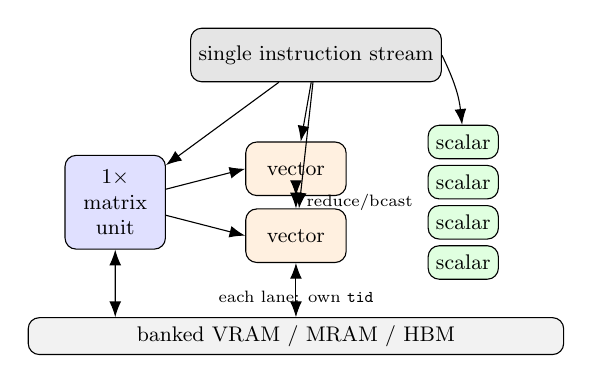
\begin{tikzpicture}[scale=0.85, transform shape, font=\small, >={Latex[length=2mm]},
  u/.style={draw, rounded corners, minimum width=1.5cm, minimum height=0.8cm, align=center}]
\node[u, fill=black!10, minimum width=3cm] (is) at (0,2.2) {single instruction stream};
\node[u, fill=blue!12, minimum height=1.4cm] (mat) at (-3,0) {1$\times$\\matrix\\unit};
\node[u, fill=orange!12] (v1) at (-0.3,0.5) {vector};
\node[u, fill=orange!12] (v2) at (-0.3,-0.5) {vector};
\node[u, fill=green!12, minimum width=1.0cm, minimum height=0.5cm] (s1) at (2.2,0.9) {scalar};
\node[u, fill=green!12, minimum width=1.0cm, minimum height=0.5cm] (s2) at (2.2,0.3) {scalar};
\node[u, fill=green!12, minimum width=1.0cm, minimum height=0.5cm] (s3) at (2.2,-0.3) {scalar};
\node[u, fill=green!12, minimum width=1.0cm, minimum height=0.5cm] (s4) at (2.2,-0.9) {scalar};
\draw[->] (is) -- (mat) node[midway,left]{};
\draw[->] (is) -- (v1); \draw[->] (is) -- (v2);
\draw[->] (is.east) to[bend left=10] (s1);
\draw[->] (mat) -- (v1.west); \draw[->] (mat) -- (v2.west);
% cross-unit reduce/broadcast between vector units
\draw[<->, dashed] (v1) -- (v2) node[midway,right=1pt]{\scriptsize reduce/bcast};
\node[align=center, below=0.3cm of v2] {\scriptsize each lane: own \texttt{tid}};
\node[u, fill=black!5, minimum width=8cm, minimum height=0.5cm] (mem) at (-0.3,-2) {banked VRAM / MRAM / HBM};
\draw[<->] (mat) -- (mem.north -| mat);
\draw[<->] (v2) -- (mem.north -| v2);
\end{tikzpicture}
\caption{The SIMT/SIMD hybrid: one matrix unit, several vector units, and
more scalar units, driven by a single instruction stream with per-lane thread
indices and a cross-unit reduce/broadcast network. Contrast with the
single-of-each SIMD baseline of Figure~\ref{fig:plena-arch}.}
\label{fig:simt-datapath}
\end{figure}

\subsection{Feeding the vector units: VRAM banking}

Replicating the vector units risks a \textbf{local memory wall}: several
vector units now want operands from the vector SRAM (VRAM) at once, and a
single VRAM port would serialise them. The fix is to \textbf{split the VRAM
into banks} --- independent sub-memories, each with its own port --- so the
vector units read \emph{concurrently}, each from its own bank, and the
aggregate VRAM$\to$vector bandwidth scales with the bank count to match the
units demanding it.

In practice this is a small change for PLENA, because the VRAM access
granularity is \emph{already} one full $\text{VLEN}$ row per access. The
memory is read a whole row at a time, so partitioning those rows across banks
aligns with how the data is already addressed --- the head-packed layout of
Section~\ref{sec:mem-angle} maps directly onto banks (different head groups in
different banks) without changing the access pattern or disturbing the
no-padding geometry. Banking is therefore the memory-side counterpart of
replicating the vector units, introduced alongside them, and it composes
cleanly with the existing row-granular reads rather than requiring a redesign
of how VRAM is accessed.

\subsection{The added instructions}

Four additions turn the baseline ISA into the hybrid, and no more were
needed:

\begin{itemize}
\item \textbf{Thread registers.} \texttt{blockIdx} and \texttt{tid} are
ordinary general-purpose registers, written and read like any other, exactly
as in a GPU's PTX. A kernel selects its slice of the work by indexing on
them; nothing else in the programming model changes.
\item \textbf{Barrier (\texttt{sync}).} A synchronisation instruction that
stalls until every parallel context has reached it. It gives the cross-unit
collectives a well-defined point at which all partial results exist.
\item \textbf{Memory barrier.} Orders the staged loads and stores of the
parallel contexts against one another, so the asynchronous copies that the
pipeline relies on (Section~\ref{sec:tiling}) remain correct when several
contexts share the memory path.
\item \textbf{Cross-unit reduce / broadcast.} The collectives that a single
vector unit did within itself --- the softmax sum, the norm statistic, the
modulation broadcast --- now span the vector units. The reduce tree and the
broadcast fan-out are extended across units, gated by the barrier above.
\end{itemize}

\subsection{Warps and the scheduler: full asynchrony}

The execution model this leads to is closely analogous to a modern NVIDIA
GPU \emph{after} the introduction of the warp-group matrix instruction
(WGMMA) on H100. The structure is the same; the difference is what the
issue slots drive. On the GPU a warp issues to load/store units and the
tensor core; here those load/store units are replaced by the device's two
real data paths --- a \textbf{matrix channel} (the systolic array) and a
\textbf{vector channel} (the vector units) --- plus the memory channel.
Threads are grouped into a \textbf{warp of 32}, and because the device issues
narrower than a warp is wide, one warp instruction takes \textbf{eight
cycles} to stream through. A \textbf{warp scheduler} holds many warps and
switches between them every issue slot, exactly as a GPU does.

% FIGURE TODO fig:simt-warp --- to be supplied:
%   warp scheduler issuing 32-thread warps over 8 cycles to three channels
%   (matrix / vector / memory); warps interleaved so that while one warp's
%   matrix op streams, another's vector op and a third's load/store run,
%   hiding all latency. (Author to add.)
\begin{figure}[t]
\centering
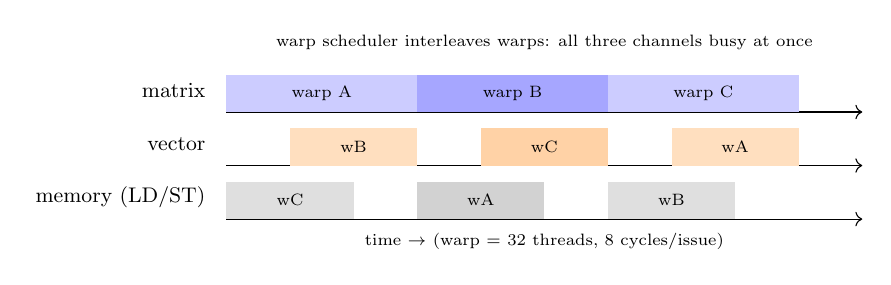
\begin{tikzpicture}[scale=0.85, transform shape, font=\small, x=0.95cm, y=0.8cm]
% three channel rows; time across; colored blocks = different warps' ops
\foreach \ch/\y/\name in {0/0/{memory (LD/ST)}, 1/1/{vector}, 2/2/{matrix}}{
  \node[left] at (-0.2,\y+0.4) {\name};
  \draw[->] (0,\y) -- (10,\y);
}
% matrix row (top): warp A, B, C streaming
\fill[blue!20] (0,2) rectangle (3,2.7); \node at (1.5,2.35){\scriptsize warp A};
\fill[blue!35] (3,2) rectangle (6,2.7); \node at (4.5,2.35){\scriptsize warp B};
\fill[blue!20] (6,2) rectangle (9,2.7); \node at (7.5,2.35){\scriptsize warp C};
% vector row (mid): different warps fill the gaps
\fill[orange!25] (1,1) rectangle (3,1.7); \node at (2,1.35){\scriptsize wB};
\fill[orange!35] (4,1) rectangle (6,1.7); \node at (5,1.35){\scriptsize wC};
\fill[orange!25] (7,1) rectangle (9,1.7); \node at (8,1.35){\scriptsize wA};
% memory row (bot)
\fill[gray!25] (0,0) rectangle (2,0.7); \node at (1,0.35){\scriptsize wC};
\fill[gray!35] (3,0) rectangle (5,0.7); \node at (4,0.35){\scriptsize wA};
\fill[gray!25] (6,0) rectangle (8,0.7); \node at (7,0.35){\scriptsize wB};
\node[below] at (5,-0.1) {\scriptsize time $\rightarrow$ (warp = 32 threads, 8 cycles/issue)};
\node[above, align=center] at (5,3) {\scriptsize warp scheduler interleaves warps: all three channels busy at once};
\end{tikzpicture}
\caption{Warp scheduling across the matrix, vector, and memory channels.
While one warp's matrix op streams, another warp's vector op and a third's
load/store run, so interleaving warps hides each channel's latency behind the
others' work --- the asynchronous pipeline.}
\label{fig:simt-warp}
\end{figure}

This warp model is what makes the device's three activities \textbf{fully
asynchronous}. By continually switching warps, the scheduler can keep the
matrix channel streaming one warp's GEMM while a second warp's vector
computation runs and a third warp's load/store moves the next tiles --- the
load/store, the matrix multiply, and the vector compute all overlapping
instead of running in series. This is the mechanism behind the latency the
SIMT sweep recovers (Section~\ref{sec:results-simt}): it is precisely the
serial dependency between the matrix and vector phases --- the barrel problem
of Section~\ref{sec:compute-angle} --- that warp interleaving dissolves. The
cost is real hardware complexity (a warp scheduler, 32-wide warp state, the
eight-cycle issue), but the complexity is in the issue logic, not in the
kernels.

\subsection{Why the hardware is harder but the use is easier}

This datapath is materially more complex than the pure-SIMD baseline: the
cross-unit reduce/broadcast network, the per-lane thread state, and the
barrier logic are all new silicon. The payoff is that, from the
\emph{programmer's and compiler's} side, almost nothing changes. Because the
thread indices are plain registers and the only new control is two barrier
instructions, the existing block-parallel lowering
(Section~\ref{sec:device-alloc}) extends to multiple contexts with no new
programming model --- the same TileLang kernels compile through the same
pipeline, now emitting \texttt{sync}/barrier where the collectives require it.
The complexity is absorbed once, in the hardware and the lowering, and hidden
from every kernel thereafter. This is the deliberate trade the design makes:
spend hardware and compiler effort once to widen the short staves, so that
every block --- and especially attention, whose vector phase was the binding
constraint --- runs closer to its matrix-bound limit without the kernel author
doing anything differently.

The three quantities this report measures are established by two
independent paths that share no code. \textbf{Latency and energy} fall
directly out of the compiled ISA (Chapter~\ref{ch:analysis}): the cycle
count comes from the instruction stream and the geometry, and the energy
from the precision-scaled power model. \textbf{Accuracy} is the harder one,
and is established through a deliberate chain that lets a fast \emph{GPU}
measurement stand in for the accelerator.

\subsection{The sim $\to$ GPU $\to$ ISA chain}
\label{sec:impl-verify}

\begin{enumerate}
\item \textbf{The simulator anchors numerical correctness.} The PLENA
transactional simulator is bit-faithful on the arithmetic (though it does
not model the pipeline finely enough for latency). A single kernel or block
is run on it and its output confirmed to match the quantised golden
reference. This validates that the quantisation convention --- per-operator
datatypes, MX/FP8 rounding, accumulation order --- is exactly what the
hardware computes, and, more fundamentally, that the from-scratch compiler's
lowering is correct: the ISA it emits, executed on the simulator, reproduces
the operator it was compiled from. Whole single- and double-stream blocks
have been run end-to-end on the simulator this way and pass to within pure
quantisation noise (Appendix~\ref{app:sim-validation}).
\item \textbf{The same quantisation is reproduced on the GPU.} The simulator
is far too slow to run a whole model. Once a kernel satisfies ``simulator
output $=$ quantised golden,'' the identical quantisation (same datatypes,
same per-operator rounding) is reproduced on the GPU. The two agree by
construction, so the GPU now stands in for the hardware on accuracy.
\item \textbf{The whole model is run on the GPU.} With every operator's
quantisation matched, the full MMDiT is run on the GPU to measure
end-to-end accuracy (cosine / NRMSE against the FP32 reference) and, just as
importantly, how the quantisation error propagates through depth and across
the denoising loop.
\item \textbf{Latency and energy come from the ISA, orthogonally.} The same
kernels are compiled to PLENA ISA and analysed for cycles and energy.
Because precision is cycle-invariant, this path is independent of the
accuracy path: they share no code and cannot mask each other's errors.
\end{enumerate}

This is why the accuracy results in Chapter~\ref{ch:results} are measured on
a GPU yet describe the PLENA deployment --- the GPU is running the
hardware-matched quantisation, anchored to the simulator on a per-kernel
basis.

As a precondition for the accuracy study, both block implementations were
first checked unquantised against a PyTorch reference at the real
dimensions; they reproduce it to the BF16 rounding floor, confirming the
kernels are correct by construction before any low-precision error is
introduced. The quantitative accuracy results --- forward correctness, FP8
quantisation, and error propagation through the denoising loop --- are
reported in Chapter~\ref{ch:results}.


% #####################################################################
% CHAPTER 5 — RESULTS AND EVALUATION
% #####################################################################
\chapter{Results}
\label{ch:results}

This chapter reports the measured results along the three axes of
Section~\ref{sec:objectives}: \textbf{accuracy}
(Section~\ref{sec:results-accuracy}), then \textbf{latency} and
\textbf{energy}. For latency and energy it works from the inside out: first
a \textbf{local}, per-kernel analysis of where each block spends its time and
energy (Section~\ref{sec:local-analysis}), then the \textbf{global} picture
--- whole blocks and the full MMDiT against the compute-matched A100, for
both inference and training (Sections~\ref{sec:results-latency} onward). The
interpretation of these numbers --- how well they meet the objectives, and
their limitations --- is the subject of Chapter~\ref{ch:evaluation}. Every
latency and energy figure comes from the compiled ISA analysed by the energy
tool of Chapter~\ref{ch:analysis} (real instruction counts, the
\texttt{customISA} cycle model, the bottom-up power model); nothing is
estimated from FLOP counts. Unless noted, the per-kernel figures are for a
\emph{single} PLENA device; the device allocation of
Section~\ref{sec:device-alloc} then divides the latency across the
deployment.

\section{Local analysis: where each kernel spends its time and energy}
\label{sec:local-analysis}

The first question is, within a block, which kernels dominate and what kind
of work they are. We answer it separately for the three stages of the model
lifecycle --- forward (inference), backward, and the optimiser --- and within
each, separately for the single-stream block (SSB) and the double-stream
block (DSB). For every kernel class we report its share of the block's
latency and of its energy, and the split of its compute between the matrix,
vector, and scalar units. Inference figures are at MX-E4M3; training
(backward and optimiser) figures are at FP32, per the precision design of
Section~\ref{sec:precision-design}.

\subsection{Forward (inference)}

\begin{table}[h]
\centering
\caption{Forward per-kernel-class breakdown, single device, MX-E4M3. ``Lat''
and ``Energy'' are shares of the block total; ``mm/vec/scl'' is the split of
that class's compute cycles across the matrix, vector, and scalar units.}
\label{tab:local-fwd}
\begin{tabular}{@{}llrrccc@{}}
\toprule
Block & Class & Lat & Energy & matrix & vector & scalar \\
\midrule
\multirow{3}{*}{SSB} & Attention & 41.6\% & 34.2\% & 60\% & 32\% & 7\% \\
 & Linear & 48.1\% & 61.6\% & 98\% & 2\% & 0\% \\
 & Other & 10.2\% & 4.2\% & 26\% & 68\% & 7\% \\
\midrule
\multirow{3}{*}{DSB} & Attention & 44.0\% & 36.6\% & 60\% & 32\% & 7\% \\
 & Linear & 45.9\% & 59.3\% & 98\% & 2\% & 0\% \\
 & Other & 10.1\% & 4.0\% & 25\% & 69\% & 7\% \\
\bottomrule
\end{tabular}
\end{table}

Table~\ref{tab:local-fwd} confirms the design analysis of
Chapter~\ref{ch:analysis} with measured numbers, and both blocks behave
almost identically. The linear kernels are the largest single share of
latency ($46$--$48\%$) and the dominant share of energy ($59$--$62\%$), and
they are essentially pure matrix work ($98\%$ on the matrix unit). Attention
is the next largest at $42$--$44\%$ of latency, and it is the only
\emph{mixed} kernel: its compute splits $60\%$ matrix, $32\%$ vector,
$7\%$ scalar --- exactly the profile that made it the hard case for compute
balance in Section~\ref{sec:compute-angle}. The seven ``other'' vector
kernels together are only ${\sim}10\%$ of latency and $4\%$ of energy, and
are vector-dominated as expected. The energy column is even more
matrix-skewed than the latency column because the matrix array is the
highest-power unit, so the linear and attention GEMMs account for
${\sim}96\%$ of energy between them.

\subsection{Backward (training)}

\begin{table}[h]
\centering
\caption{Backward per-kernel-class breakdown, single device, FP32. Columns
as in Table~\ref{tab:local-fwd}.}
\label{tab:local-bwd}
\begin{tabular}{@{}llrrccc@{}}
\toprule
Block & Class & Lat & Energy & matrix & vector & scalar \\
\midrule
\multirow{3}{*}{SSB} & Attention & 34.1\% & 36.4\% & 94\% & 6\% & 0\% \\
 & Linear & 54.2\% & 60.5\% & 99\% & 1\% & 0\% \\
 & Other & 11.7\% & 3.1\% & 11\% & 83\% & 6\% \\
\midrule
\multirow{3}{*}{DSB} & Attention & 31.0\% & 32.6\% & 94\% & 6\% & 0\% \\
 & Linear & 59.2\% & 64.9\% & 99\% & 1\% & 0\% \\
 & Other & 9.8\% & 2.5\% & 11\% & 83\% & 6\% \\
\bottomrule
\end{tabular}
\end{table}

The backward pass (Table~\ref{tab:local-bwd}) shifts the balance further
towards the linear kernels: because every forward linear becomes two
backward GEMMs, the linear class grows to $54$--$59\%$ of latency and
$60$--$65\%$ of energy. Attention's share of latency falls to $31$--$34\%$,
and --- notably --- its internal split moves to $94\%$ matrix, against only
$60\%$ in the forward. The reason is specific: the forward attention must
run the \emph{full} online softmax, whose row-wise \texttt{max} and
\texttt{sum} reductions are heavy vector operations (they dominate its $32\%$
vector share). The backward does \emph{not} redo that work --- it reuses the
softmax statistics ($L$, $D$) saved from the forward and only needs a cheap
element-wise rescale, with no row reductions. With the expensive reduce
removed and two extra GEMMs added (five in total), attention's backward is
almost pure matrix work. The ``other'' (vector) kernels stay small in
energy ($2$--$3\%$) but their backward forms are more vector-heavy
($83\%$) than their forward forms, reflecting the extra reductions that
normalisation backward requires (Section~\ref{sec:impl-backward}).

\subsection{Optimiser (AdamW)}

The optimiser step is, by design, negligible next to the forward and
backward passes. The AdamW kernel is a single element-wise vector pass over
each weight tensor: on one device it runs in ${\sim}0.23$\,ms and consumes
${\sim}0.7$\,mJ, with \emph{zero} matrix work --- all of it on the vector
unit. For comparison, one SSB backward pass is ${\sim}534$\,ms and
${\sim}9.5$\,J on the same device, so the optimiser is roughly four orders
of magnitude smaller and does not appear in the training cost in any
meaningful way. It is reported here for completeness; it plays no role in
the global analysis that follows.

\paragraph{Summary of the local picture.} Across all three stages the story
is the same: \textbf{the matrix kernels --- linears and attention --- are
essentially all of the cost}, carrying ${\sim}96\%$ of energy in the
forward and ${\sim}97\%$ in the backward, while the vector kernels are a
small latency overhead and a negligible energy one. Attention is the only
kernel that exercises all three units, and the optimiser is immaterial. The
global results that follow therefore track the matrix throughput almost
directly.

\section{Accuracy}
\label{sec:results-accuracy}

Before latency and energy, the first axis is accuracy: does the model still
produce correct outputs once its arithmetic is mapped onto the
accelerator's low-precision datapath? All accuracy numbers are measured on
the GPU running the hardware-matched quantisation, anchored to the simulator
per kernel (the methodology of Section~\ref{sec:impl-verify}), and reported
as cosine similarity and NRMSE against the FP32 reference.

\subsection{Forward numerical correctness}

As a baseline, the unquantised TileLang blocks reproduce the PyTorch
reference essentially exactly: the single-stream block to cosine
$1.000000$, and the two double-stream streams to $0.999999$, with the
residual error at the BF16 rounding floor rather than any algorithmic
discrepancy. The implementations are therefore correct by construction, and
what follows measures only the cost of low precision.

\subsection{FP8 quantisation of the whole MMDiT}

On the real Open-Sora weights, quantising to FP8 (E4M3) and measuring the
output against the FP32 teacher gives Table~\ref{tab:fp8-accuracy}. Two
granularities are shown: weight-only (W8A16) and weight-plus-activation
(W8A8, both GEMM operands FP8).

\begin{table}[h]
\centering
\caption{FP8 (E4M3) accuracy on the real Open-Sora weights, against the
FP32 reference. PTQ is plain post-training quantisation (no weight update);
QAT is short scale-only quantisation-aware fine-tuning.}
\label{tab:fp8-accuracy}
\begin{tabular}{@{}lcc@{}}
\toprule
Scheme & PTQ cosine & QAT cosine \\
\midrule
W8A16 (weight-only) & 0.99973 & 0.99976 \\
W8A8 (weight + activation) & 0.99944 & 0.99948 \\
\bottomrule
\end{tabular}
\end{table}

The result is that \textbf{8-bit (E4M3) is a near-lossless operating point}.
With per-output-channel scale calibration, plain PTQ already reaches cosine
\textbf{0.9997} (weight-only) and \textbf{0.9994} (W8A8) \emph{with no
fine-tuning}. Short scale-only fine-tuning closes the residual to numerically
indistinguishable from FP32, but is not required. (Letting fine-tuning also
update the weights overfits an already-perfect point and \emph{drops} the
cosine to ${\sim}0.91$; in the 8-bit safe zone the correct recipe is to tune
the scales only.)

\subsection{Error does not accumulate with depth or over the loop}

A single block being near-lossless is not sufficient: real inference is a
denoising loop of many steps, each a full MMDiT forward (19 DSB then 38 SSB,
${\sim}456$ large FP8 GEMMs per forward), whose output feeds the next step.
FP8 error could in principle accumulate along \emph{two} axes --- model
depth and loop time. Stacking the real-depth backbone and running a 30-step
rectified-flow loop, comparing the FP8 latent against FP32 at each step,
shows it does not:

\begin{table}[h]
\centering
\caption{FP8 vs.\ FP32 latent across a 30-step denoising loop at the real
backbone depth (57 blocks). The error is frozen from the first step.}
\label{tab:error-prop}
\begin{tabular}{@{}lcc@{}}
\toprule
Denoising step & cosine & NRMSE \\
\midrule
1 (first full forward) & 0.999381 & 0.0352 \\
6 & 0.999360 & 0.0358 \\
15 & 0.999360 & 0.0358 \\
30 (final latent) & 0.999360 & 0.0358 \\
\bottomrule
\end{tabular}
\end{table}

\textbf{FP8 error accumulates along neither axis.} Across 57 blocks of depth
the cosine holds at $0.9994$ --- the residual structure routes FP8 noise only
into the block's ``out'' branch, leaving the trunk lossless --- and across
the 30-step loop it is frozen at $0.99936$ (step 1 to 30 changes by
$+0.00002$). Sampling is a convergence process: the scheduler pulls the
latent back to the data manifold each step, so the ${\sim}3.5\%$ FP8 noise is
diluted, not amplified. \textbf{The whole Open-Sora model runs FP8 inference
with zero fine-tuning at a final-latent cosine of $0.9994$.}

\subsection{Accumulation precision confirms the power model}

Finally, the whole-MMDiT FP8 result under the two accumulation choices the
matmul datapath can use (FP8 products feeding an FP32 or an FP16
accumulator):

\begin{center}
\begin{tabular}{@{}lcc@{}}
\toprule
Whole MMDiT (FP8) & cosine & NRMSE \\
\midrule
FP8 + FP32 accumulation & 0.999457 & 0.0330 \\
FP8 + FP16 accumulation & 0.999448 & 0.0332 \\
\bottomrule
\end{tabular}
\end{center}

\noindent The accumulation precision \textbf{barely matters}: the gap between
FP32 and FP16 accumulation is $0.00001$ in cosine. This is the accuracy
counterpart to the power model's two-leg split
(Section~\ref{sec:precision-design}): because FP8 can accumulate into FP16
with no measurable accuracy loss, the matrix array stays at its FP16
accumulator --- the $1\times$ power point --- for FP8 inference rather than
paying for an FP32 accumulator. The accuracy measurement confirms exactly
what the energy model assumes.

\section{Inference: per-block latency and energy against the A100}
\label{sec:results-latency}

We now assemble the kernels into whole blocks and measure them against the
compute-matched A100 (Section~\ref{sec:a100-match}). All PLENA figures are
at the 12-device, BLEN-8 deployment; latency falls as $1/N$ with device
count while \textbf{total energy is unchanged} (the same work spread across
more silicon), so the energy advantage is independent of how many devices
are deployed. The A100 reference is its fastest result, PyTorch + scaled
dot-product attention. Speedup is A100\,latency\,/\,PLENA\,latency; the
energy ratio is A100\,energy\,/\,PLENA\,energy (above 1 means PLENA wins).

\subsection{Why the comparison runs at batch 4}
\label{sec:batch4}

A point that all the comparisons below depend on: \textbf{both sides are run
at batch 4}, and this is required for the A100 baseline to be \emph{fair}
rather than artificially slow. The A100 has 108 streaming multiprocessors,
and a GPU only reaches its peak throughput when every SM is given work ---
the launch grid must expose at least as many thread-blocks as there are SMs
($\ge 108$). At the Open-Sora dimensions a \emph{single} batch element does
not produce enough thread-blocks to cover all the SMs, so the A100 would sit
partly idle and report a misleadingly slow time. A batch of 4 pushes the
block count past the SM threshold and \textbf{saturates the GPU}, which is
the A100's best (most favourable) operating point. Comparing PLENA against a
\emph{saturated} A100 is the honest comparison; comparing against an
under-filled one would flatter PLENA. Batch 4 is therefore the shape used
for every per-block and per-pass result in this chapter.

The full \emph{generation} shape is larger still. Each denoising step issues
one MMDiT forward carrying the \textbf{classifier-free-guidance (CFG)}
branches --- the sampler concatenates 3 conditioning versions of the latent
(text-conditioned, image-conditioned, unconditional) into one batched
forward. Combined with the batch-4 GPU-fill, the effective batch per forward
at generation time is
\[
\text{batch} = 3\,(\text{CFG}) \times 4\,(\text{GPU fill}) = 12,
\]
and a generation is 50 such steps. The per-block tables use batch 4; the
generation totals (Section~\ref{sec:results-full}) use batch 12. Energy
scales linearly with batch and is independent of device count, so both
follow directly from the per-block numbers.

\subsection{The A100 baseline}
\label{sec:a100-baseline}

The A100 reference is established by running the same blocks on the GPU
itself, both as our own TileLang kernels and as the standard PyTorch +
scaled-dot-product-attention (SDPA) path, isolating kernel quality on the
GPU before any move to PLENA:

\begin{table}[h]
\centering
\caption{A100-80GB per-block baseline (BF16, batch 4): our TileLang kernels
vs.\ the PyTorch + SDPA reference. The fastest GPU result (PyTorch + SDPA)
is the baseline used for the PLENA comparison.}
\label{tab:a100-baseline}
\begin{tabular}{@{}llrrr@{}}
\toprule
Block & Implementation & Latency & Power & Energy \\
\midrule
\multirow{2}{*}{SSB} & PyTorch + SDPA & \textbf{73.4\,ms} & 393\,W & \textbf{28.9\,J} \\
 & TileLang (ours) & 85.1\,ms & 388\,W & 33.0\,J \\
\multirow{2}{*}{DSB} & PyTorch + SDPA & \textbf{87.4\,ms} & 391\,W & \textbf{34.2\,J} \\
 & TileLang (ours) & 101.1\,ms & 440\,W & 44.5\,J \\
\bottomrule
\end{tabular}
\end{table}

Our hand-written TileLang kernels land at \textbf{$0.86\times$} the speed of
PyTorch + SDPA for both blocks --- within ${\sim}15\%$ of the heavily-tuned
vendor library. This sets the GPU reference point and, importantly, fixes
the \emph{most demanding} A100 baseline: the PLENA comparison below uses the
\emph{faster} PyTorch + SDPA numbers, not our own TileLang GPU result, so
PLENA is measured against the strongest GPU figure available.

\begin{table}[h]
\centering
\caption{Per-block forward (inference, MX-E4M3, batch 4) vs.\ A100, swept
over PLENA device count. Energy is constant across the sweep; latency
divides by device count.}
\label{tab:fwd-vs-a100}
\begin{tabular}{@{}lrrrrr@{}}
\toprule
Config & Lat (ms) & Energy (J) & Power (W) & Speedup & Energy ratio \\
\midrule
\multicolumn{6}{@{}l}{\emph{SingleStreamBlock}}\\
A100 (PyTorch+SDPA) & 73.4 & 28.9 & 393 & 1.00$\times$ & 1.00$\times$ \\
PLENA --- 1 device & 1077.7 & 8.44 & 7.8 & 0.07$\times$ & 3.42$\times$ \\
PLENA --- 4 devices & 269.4 & 8.44 & 31.2 & 0.27$\times$ & 3.42$\times$ \\
\textbf{PLENA --- 12 devices} & \textbf{89.8} & \textbf{8.44} & 93.6 & \textbf{0.82$\times$} & \textbf{3.42$\times$} \\
\midrule
\multicolumn{6}{@{}l}{\emph{DoubleStreamBlock}}\\
A100 (PyTorch+SDPA) & 87.4 & 34.2 & 391 & 1.00$\times$ & 1.00$\times$ \\
PLENA --- 1 device & 1257.7 & 9.75 & 7.8 & 0.07$\times$ & 3.51$\times$ \\
PLENA --- 4 devices & 314.4 & 9.75 & 31.2 & 0.28$\times$ & 3.51$\times$ \\
\textbf{PLENA --- 12 devices} & \textbf{104.8} & \textbf{9.75} & 93.6 & \textbf{0.83$\times$} & \textbf{3.51$\times$} \\
\bottomrule
\end{tabular}
\end{table}

Table~\ref{tab:fwd-vs-a100} gives the headline inference result. Two things
stand out. First, \textbf{energy is the decisive win}: at a matched MAC
budget PLENA uses \textbf{3.4$\times$ (SSB) / 3.5$\times$ (DSB) less energy}
per block than the A100, and because adding devices does not change total
energy, this advantage holds at every point on the sweep, at roughly a
\emph{quarter} of the A100's average power. Second, \textbf{latency reaches
${\sim}0.8\times$ of the A100} at the 12-device match ($0.82\times$ SSB,
$0.83\times$ DSB --- within ${\sim}20\%$), using device-level parallelism
alone. Device scaling is clean and linear: latency divides by device count
at fixed energy, so the deployment can be dialled to any latency target by
trading aggregate power for speed.

\section{Memory: the workload is compute-bound, even split across 12 devices}
\label{sec:results-memory}

The latency comparison above only holds if PLENA is genuinely
\emph{compute-bound} --- if the matrix core, not the memory system, is the
limiting resource. This is the design intent established in
Section~\ref{sec:mem-angle}; here it is verified with measured traffic, and
the verification is pushed to its hardest case: many devices contending for
one shared HBM.

\paragraph{Bandwidth available.} PLENA moves data between HBM and the
on-chip SRAMs over two DMA ports --- a matrix port and a vector port, each
$\text{MLEN}/\text{VLEN}$-wide per cycle:
\[
\text{per-port BW} = 1024\,\text{B/cyc}\times1.0\,\text{GHz} = 1024\,\text{GB/s},
\qquad \text{total} \approx 2{,}048\,\text{GB/s}.
\]
This is in the same class as the A100-80GB's HBM2e ($2{,}039$\,GB/s), so the
comparison does not bias PLENA with an unrealistic memory subsystem.

\paragraph{Traffic per block.} All HBM tensors are MX-E4M3 (8-bit element +
E8M0 block scale, a $1.25\times$ byte overhead). Dividing per-block traffic
by the available bandwidth gives the memory time, which is minute next to
the single-device compute time:

\begin{table}[h]
\centering
\caption{Per-block HBM traffic versus compute time (batch 4, one device).
Memory is three to four orders of magnitude below compute.}
\label{tab:mem-traffic}
\begin{tabular}{@{}lrrrr@{}}
\toprule
Block & HBM traffic & Memory time & Compute (1 dev) & Mem / compute \\
\midrule
SSB & 356\,MB & 0.35\,ms & 1077.7\,ms & \textbf{0.03\%} \\
DSB & 509\,MB & 0.50\,ms & 1257.7\,ms & \textbf{0.04\%} \\
\bottomrule
\end{tabular}
\end{table}

\paragraph{Worst-case contention across 12 devices.} The interesting case is
the 12-device deployment, where a block is \emph{split} across devices, not
replicated --- so the total HBM traffic is fixed at one block's worth, just
partitioned into per-device shares. What changes is that all 12 devices want
to read the shared HBM at once, so accesses must queue. We take the most
pessimistic possible model: a single shared HBM pool at $2{,}039$\,GB/s with
every device's traffic \emph{fully serialised} through it (round-robin, one
device at a time, \emph{no} concurrent access at all), and compare the
resulting HBM-busy time against the per-block latency at 12 devices.

\begin{table}[h]
\centering
\caption{Worst-case HBM contention: one block split across 12 devices, all
traffic forced through a single $2{,}039$\,GB/s pool with zero concurrency.
The shared HBM is busy ${\sim}0.2\%$ of the wall-clock.}
\label{tab:hbm-contention}
\begin{tabular}{@{}lrrrr@{}}
\toprule
Block & Total traffic & HBM busy (serialised) & Latency (12 dev) & HBM duty cycle \\
\midrule
SSB & 356\,MB & 0.17\,ms & 89.81\,ms & \textbf{0.19\%} \\
DSB & 509\,MB & 0.24\,ms & 104.81\,ms & \textbf{0.23\%} \\
\bottomrule
\end{tabular}
\end{table}

Even in this worst case --- every HBM access pushed through one pipe with no
concurrency --- the shared HBM is busy only ${\sim}0.2\%$ of the wall-clock,
leaving \textbf{${\sim}430$--$530\times$ headroom}. Because the work is split
rather than replicated, the bytes to move never grow with device count;
queuing only reorders a few hundred megabytes in time, and there is far more
than enough bandwidth to drain the queue before the compute needs the data.
Twelve devices in parallel demand under $5$\,GB/s aggregate --- about
$0.2\%$ of one A100's HBM bandwidth.

The implication closes the latency argument: memory time is three to four
orders of magnitude below compute time, so under the overlapped
$\text{total}=\max(\text{compute},\text{memory})$ model every kernel is
compute-bound and the DMA traffic hides completely behind computation. The
latency and energy numbers are therefore governed entirely by the
matrix/vector compute, and device-level scaling does not stress aggregate
bandwidth. This is exactly the regime --- dense, high-arithmetic-intensity
GEMMs and attention, each HBM byte reused across many MACs --- that a
systolic matrix core is built to exploit, and it is the measured
confirmation of the no-padding, high-bandwidth memory design of
Section~\ref{sec:mem-angle}.

\section{Inference: the full MMDiT pass and a full generation}
\label{sec:results-full}

A block is not the end-to-end cost. The full MMDiT pass is
$38\,\text{SSB} + 19\,\text{DSB} + \text{final layer}$, and a generation
runs that pass once per denoising step.

\paragraph{The per-component split confirms the design judgement.}
\label{sec:results-finallayer}
Measured on the compiled ISA, the single- and double-stream blocks are
\textbf{99.97\%} of the pass (SSB $63\%$, DSB $37\%$), and the
\textbf{final layer is $0.03\%$} of both latency and energy. This is the
measured confirmation of the decision in Section~\ref{sec:edge} to implement
the final layer for functional correctness but exclude it from the cost
analysis: at $0.03\%$ it is three orders of magnitude below the blocks, so
ignoring it in every latency and energy figure introduces no error, while the
$99.97\%$ that \emph{is} the two block types is exactly what the acceleration
effort targeted. The per-block results therefore carry straight through to
the full pass.

\begin{table}[h]
\centering
\caption{Full MMDiT forward pass and one full 256px generation (50 steps,
batch $3\,\text{CFG}\times4 = 12$): PLENA (12 devices) vs.\ A100.}
\label{tab:full-mmdit}
\begin{tabular}{@{}lrrr@{}}
\toprule
 & A100 & PLENA (12 dev) & Ratio \\
\midrule
MMDiT pass --- latency & 4.45\,s & 5.41\,s & 0.82$\times$ \\
MMDiT pass --- energy & 1{,}748\,J & \textbf{506\,J} & \textbf{3.45$\times$ less} \\
MMDiT pass --- avg power & 393\,W & 93.6\,W & --- \\
\midrule
Full generation --- latency & 667.5\,s (11.1\,min) & 810.8\,s (13.5\,min) & 0.82$\times$ \\
Full generation --- energy & 262.2\,kJ & \textbf{75.9\,kJ} & \textbf{3.45$\times$ less} \\
\bottomrule
\end{tabular}
\end{table}

Table~\ref{tab:full-mmdit} carries the result to the end-to-end scale.
Generating one 256px clip drives the backbone for 50 steps; a 12-device
PLENA completes it at \textbf{0.82$\times$ the A100's speed} (13.5 vs
11.1 minutes) while consuming \textbf{75.9\,kJ against 262.2\,kJ --- a
$3.45\times$ reduction in generation energy} --- at a quarter of the average
power. Because the MMDiT is $99.4\%$ of generation FLOPs
(Section~\ref{sec:compute-breakdown}), this is effectively the energy
profile of the whole model. The latency gap is the cost of running at a
matched, not larger, MAC budget; it can be closed in two ways: by deploying
more devices (latency $\div N$ at the same energy), or by raising the SIMT
width, as the next subsection shows.

\subsection{Closing the latency gap with SIMT}
\label{sec:results-simt}

The per-pass figures above are at SIMT $=1$ (pure SIMD, no thread-level
widening). PLENA also supports a SIMT mode that overlaps the vector tail of
the pipeline; raising the SIMT width trims latency until the pass becomes
fully matmul-bound, while leaving energy essentially unchanged.

\begin{table}[h]
\centering
\caption{Full MMDiT pass (12 devices, batch 4) swept over SIMT width.
Energy is essentially flat; SIMT only trims the vector tail of latency,
after which the pass is matmul-bound.}
\label{tab:simt-sweep}
\begin{tabular}{@{}rrrr@{}}
\toprule
SIMT & Latency (s) & Energy (J) & Avg power (W) \\
\midrule
1 & 5.41 & 506 & 93.6 \\
2 & 4.72 & 499 & 105.6 \\
4 & 4.38 & 495 & 113.0 \\
8 & 4.21 & 493 & 117.2 \\
16 & 4.12 & 492 & 119.4 \\
32 & 4.08 & 492 & 120.5 \\
\bottomrule
\end{tabular}
\end{table}

Table~\ref{tab:simt-sweep} shows the energy flat at ${\sim}492$--$506$\,J
across the whole sweep, confirming that SIMT trades nothing on energy ---
it only hides the vector tail behind the matrix work, with the pass becoming
matmul-bound past SIMT $=4$. The effect on the A100 comparison is decisive:
against the A100's $4.45$\,s pass, PLENA moves from $5.41$\,s ($0.82\times$)
at SIMT $=1$ to $4.08$\,s at SIMT $=32$, \textbf{crossing over to
$1.09\times$ --- faster than the A100} --- at the same ${\sim}3.5\times$
energy advantage ($492$\,J vs $1{,}748$\,J). So at a matched MAC budget PLENA
can either match the A100's energy at $0.82\times$ its speed, or beat it on
\emph{both} latency and energy once SIMT is engaged; the latency gap of the
SIMT$=1$ numbers is not fundamental. \textbf{The SIMT sweep is an analytic
latency projection, not yet verified on a cycle-accurate simulator}
(Section~\ref{sec:simt-status}): its ISA, compiler, and analytic model are in
place, but the confirming simulator is future work
(Section~\ref{sec:future}). The headline result of this report is therefore
the \emph{measured} SIMT$=1$ figure ($0.82\times$ latency at ${\sim}3.5\times$
energy); the $>$$1\times$ crossover is the projected upside. (SIMT is also not
yet integrated into the training measurements, which are at SIMT $=1$.)

\section{Training: backward and optimiser}
\label{sec:results-training}

Training runs the backward pass and the optimiser, both at FP32. The
backward inherits the same clean device scaling; the difference from
inference is precision --- FP32 doubles the per-unit power
(Section~\ref{sec:precision-design}), which narrows the energy advantage.

\begin{table}[h]
\centering
\caption{Per-block backward (training, FP32, batch 4) vs.\ A100 (PyTorch
autograd, BF16 storage / FP32 accumulate), at the 12-device deployment.}
\label{tab:bwd-vs-a100}
\begin{tabular}{@{}lrrrr@{}}
\toprule
Backward & Lat (ms) & Energy (J) & Speedup & Energy ratio \\
\midrule
A100 --- SSB & 167.5 & 64.5 & 1.00$\times$ & 1.00$\times$ \\
PLENA (12 dev) --- SSB & 178.0 & \textbf{37.9} & 0.94$\times$ & \textbf{1.70$\times$} \\
A100 --- DSB & 195.7 & 74.3 & 1.00$\times$ & 1.00$\times$ \\
PLENA (12 dev) --- DSB & 241.6 & \textbf{52.4} & 0.81$\times$ & \textbf{1.42$\times$} \\
\bottomrule
\end{tabular}
\end{table}

The backward mirrors the forward (Table~\ref{tab:bwd-vs-a100}): at a matched
MAC budget PLENA delivers \textbf{1.4--1.7$\times$ lower energy} per backward
block at \textbf{0.8--0.9$\times$} of A100 latency. The advantage is smaller
than the forward's ${\sim}3.5\times$ for exactly one reason: training runs at
high precision (FP32, unit powers $\times2$) while inference runs
low-precision (MX-E4M3, $\times1$). Against the GPU's BF16 backward, the
doubled-power PLENA still wins on energy, just by the narrower $1.4$--$1.7\times$.

\paragraph{Even more matmul-bound than the forward.} Both backward chains
are \emph{more} matmul-bound than the forward --- $87$--$89\%$ of compute is
the matrix opcodes (the plain \texttt{M\_MM} of every $dX$, the transpose-A
\texttt{M\_TMM\_A} of every $dW$ and attention's $dQ$, the score-grad
\texttt{M\_BTMM}, and their \texttt{M\_MM\_WO} drains), against ${\sim}66\%$ in
the forward --- because the five-GEMM attention backward and the two-GEMM
linear backwards add matrix work without adding much vector work (the softmax
reductions are not redone, Section~\ref{sec:local-analysis}). The MCU consequently carries ${\sim}80\%$
of backward energy and the vector unit under $1\%$. Table~\ref{tab:bwd-totals}
collects the per-block and whole-pass backward figures.

\begin{table}[h]
\centering
\caption{Backward (FP32) per-block and whole-MMDiT totals. Per-block is
batch 4; the whole-MMDiT pass is $38\,\text{SSB}+19\,\text{DSB}$. Energy is
independent of device count; latency divides by device count.}
\label{tab:bwd-totals}
\begin{tabular}{@{}lrrr@{}}
\toprule
Backward & 1 device & 12 devices & matmul share \\
\midrule
SSB --- latency & 533.9\,ms & 44.5\,ms & \multirow{2}{*}{87.1\%} \\
SSB --- energy & 9.48\,J & 9.48\,J & \\
DSB --- latency & 724.7\,ms & 60.4\,ms & \multirow{2}{*}{88.9\%} \\
DSB --- energy & 13.09\,J & 13.09\,J & \\
\midrule
Whole MMDiT --- energy (batch 1) & \multicolumn{2}{c}{\textbf{609\,J}} & --- \\
Whole MMDiT --- energy (batch 12) & \multicolumn{2}{c}{\textbf{${\sim}7.31$\,kJ}} & --- \\
\bottomrule
\end{tabular}
\end{table}

The whole-MMDiT backward's per-component split shifts slightly from the
forward's $63/37$ towards \textbf{$59.6\%$ SSB $/ 40.4\%$ DSB}, as the
double-stream block's two streams and larger joint attention make its
backward relatively more matrix-heavy.

\subsection{Optimiser step (AdamW)}
\label{sec:results-adamw}

The second part of training is the optimiser step that consumes the
gradients and updates the weights. For the MMDiT this is an AdamW update:
element-wise moment accumulation, bias correction, the decoupled-weight-decay
update, and the $1/(\sqrt{\hat v}+\epsilon)$ rescaling. It is \textbf{pure
vector work --- no matmul} --- so its cost scales with the \emph{parameter
count}, not the sequence length or batch: the optimiser touches each weight
once per step regardless of how large a batch the forward and backward ran.

The AdamW kernel was compiled to PLENA ISA and measured; per element it is
$0.314$\,nJ / $0.110$\,ns (FP32). The full MMDiT has \textbf{8.611\,billion}
trainable parameters (38 SSB + 19 DSB, $50/50$ by parameter mass), giving
one full optimiser step:

\begin{table}[h]
\centering
\caption{One full AdamW step over the 8.611\,B-parameter MMDiT (FP32).
Energy is independent of device count; latency divides by device count.}
\label{tab:adamw}
\begin{tabular}{@{}lrrr@{}}
\toprule
AdamW step (8.611\,B params) & Latency & Energy & matmul \\
\midrule
PLENA --- 1 device & 950.1\,ms & 2.710\,J & 0 \\
\textbf{PLENA --- 12 devices} & \textbf{79.2\,ms} & \textbf{2.710\,J} & 0 \\
\bottomrule
\end{tabular}
\end{table}

The energy is matmul-free: $63.8\%$ sits in the vector SRAM, $36.2\%$ in the
vector unit, the MCU idle. As a cross-check, an A100 AdamW
\texttt{optimizer.step()} over one SSB block's $141.6$\,M BF16 parameters
measures \textbf{4.01\,ms / 1.13\,J} at $282$\,W --- well below the
${\sim}384$\,W of its backward, exactly the bandwidth-bound profile expected
of a GEMM-free element-wise update.

\textbf{The optimiser is a negligible tail on the training step.} Against
the full-MMDiT backward (Table~\ref{tab:bwd-totals}, batch 4, 12 devices:
${\sim}11.4$\,s / ${\sim}2.44$\,kJ), the AdamW step is \textbf{0.079\,s /
2.71\,J} --- under \textbf{1\% of the latency and ${\sim}0.1\%$ of the
energy}. Training cost is the backward; the optimiser barely registers.

\section{Power-model validation}
\label{sec:results-power}

Every energy figure above rests on the bottom-up per-unit power model
(1\,mW/MAC, 0.5\,mW/vector-lane, 0.055\,pJ/bit SRAM;
Section~\ref{sec:precision-design}). These are cross-validated against an
independent Design-Compiler synthesis fit in Appendix~\ref{app:power}: the
vector unit and both SRAMs agree to within ${\sim}1.3\times$, and the matrix
core --- which carries ${\sim}88\%$ of energy --- agrees once a known
$M^2$-scaling bug in the synthesis fit is corrected (it disagrees by
$34\times$ uncorrected; Appendix~\ref{app:power} shows the bug, and the fit's
own near-linear area model confirms the correction). The \emph{relative}
PLENA-vs-A100 energy ratios reported throughout this chapter are robust to
the residual activity-factor uncertainty, because both sides scale together;
the \emph{absolute} watts are a lower-to-nominal bound. The headline
conclusions --- ${\sim}3.5\times$ lower inference energy, $1.4$--$1.7\times$
lower training energy, at ${\sim}0.8\times$ latency on a matched budget ---
are therefore solid.

\section{The ideal-asynchrony limit}
\label{sec:results-ideal}

Finally, we bound how much the SIMT/SIMD hybrid of
Section~\ref{sec:impl-simt} could win by overlapping the matrix, vector, and
memory channels. The right way to count this is \textbf{per kernel}: within a
kernel the three channels can overlap, so the kernel's ideal time is the
\emph{maximum} of its matrix, vector, and memory times; across kernels the
times still add. Crucially, a \emph{pure} vector kernel (LayerNorm, GELU,
RoPE, the gates) has no matrix work to hide behind, so its vector time
survives in full --- only kernels that mix the two (above all attention) gain
from overlap. Summing the per-kernel maxima gives the limit in
Table~\ref{tab:ideal-async}.

\begin{table}[h]
\centering
\caption{Ideal-asynchrony latency, counted per kernel: each kernel's time
becomes $\max(\text{matrix},\text{vector},\text{memory})$ and the kernels are
summed. Pure vector kernels keep their full time; only mixed kernels overlap.
Measured from the compiled ISA (one device).}
\label{tab:ideal-async}
\begin{tabular}{@{}lrrr@{}}
\toprule
& Serial (now) & Ideal ($\Sigma$ per-kernel max) & Reduction \\
\midrule
SSB forward & 269.4\,ms & \textbf{222.1\,ms} & \textbf{17.6\%} \\
DSB forward & 314.4\,ms & \textbf{256.1\,ms} & \textbf{18.5\%} \\
SSB backward & 533.9\,ms & \textbf{519.6\,ms} & \textbf{2.7\%} \\
DSB backward & 724.7\,ms & \textbf{706.1\,ms} & \textbf{2.6\%} \\
\bottomrule
\end{tabular}
\end{table}

Within a kernel, the achievable reduction is \textbf{${\sim}18\%$ on the
forward} and only \textbf{${\sim}2.7\%$ on the backward}. The forward gains
because attention is a large mixed kernel whose softmax vector phase hides
behind its GEMMs; the backward gains almost nothing because it is already
${\sim}88\%$ matrix-bound (Section~\ref{sec:local-analysis}) --- its attention
backward reuses the saved softmax statistics and so carries little vector work
to overlap. Over a full forward pass the per-kernel limit is a $17.9\%$
reduction ($16.2$\,s $\to 13.3$\,s on one device).

This per-kernel figure is a \emph{conservative} bound, because it allows
overlap only \emph{inside} a kernel. The warp scheduler of
Section~\ref{sec:impl-simt} can do more: by interleaving warps across kernel
boundaries it can hide one kernel's vector tail (a LayerNorm, say) behind the
\emph{next} kernel's matrix work. This is why the measured SIMT sweep
(Section~\ref{sec:results-simt}) reaches a larger $24.6\%$ reduction on the
full pass ($5.41$\,s $\to 4.08$\,s) than the $17.9\%$ within-kernel limit:
cross-kernel overlap recovers the pure-vector tails that per-kernel overlap
cannot. Either way the ceiling is the same --- the matrix channel, which the
hybrid cannot beat but can almost fully expose by removing the serial vector
and memory time from the critical path.

\paragraph{What the ideal time is made of.} It is worth being precise about
where the SSB ideal of $222.1$\,ms comes from, because it is \emph{not} just
the matrix channel. It splits into two parts:
\[
\underbrace{202.2\,\text{ms}}_{\text{matrix-bearing kernels}}
\;+\;
\underbrace{19.9\,\text{ms}}_{\text{pure vector kernels}}
\;=\; 222.1\,\text{ms}.
\]
The matrix-bearing kernels (the linears and attention) each have more matrix
than vector work, so their $\max$ is the matrix time and their vector phase
hides for free --- this group's total is exactly the matrix channel,
$202.2$\,ms. But the \textbf{pure vector kernels} (LayerNorm, QK-norm, GELU,
modulation, the gates) have \emph{no} matrix work to hide behind, so their
$19.9$\,ms cannot be overlapped and survives in full. The ideal time is the
matrix channel \emph{plus} this irreducible vector tail; overlap removes the
vector work that sits next to matrix work, not the vector work that stands
alone.

\section{Specialised devices: an energy estimate}
\label{sec:results-specialised}

Section~\ref{sec:specialised-devices} proposed routing each kernel class to a
device specialised for it. We make that concrete with three device variants,
each stripped down to exactly what its kernel class needs, and estimate the
energy of running the blocks across them.

\paragraph{The three device variants.} The configuration follows directly
from which units each kernel class exercises:

\begin{itemize}
\item \textbf{Attention device --- full.} Attention uses the matrix array,
the vector unit, and both SRAMs (it streams Q/K/V, runs the softmax, and
mixes the values), so its device is the unchanged general device. It is the
one kernel that justifies the complete datapath.
\item \textbf{Linear device --- matrix array, small SRAM.} A linear is a
pure tiled GEMM that reuses each loaded tile across the whole contraction, so
it needs the matrix array but only a little SRAM staging. It keeps the full
matrix array and matrix SRAM path but with \emph{small} VRAM and MRAM.
\item \textbf{Vector device --- no matrix array, no MRAM.} The vector
kernels never touch the matrix array, so a vector device drops the matrix
array (MCU) and the matrix SRAM (MRAM) entirely, keeping only the vector unit
and a small VRAM.
\end{itemize}

\begin{table}[h]
\centering
\caption{Specialised-device settings: which units each variant carries,
relative to the general device. ``--'' means the unit is removed; ``small''
means a reduced-capacity SRAM.}
\label{tab:specialised-settings}
\begin{tabular}{@{}lcccc@{}}
\toprule
Variant (kernel class) & Matrix array & Vector unit & MRAM & VRAM \\
\midrule
General (baseline) & full & full & full & full \\
\textbf{Attention} & full & full & full & full \\
\textbf{Linear} & full & full & small & small \\
\textbf{Vector} & --- (removed) & full & --- (removed) & small \\
\bottomrule
\end{tabular}
\end{table}

We estimate the energy of this configuration from the same per-kernel unit
breakdown used above: removing a unit removes its energy, and the shrunk
SRAMs are estimated at half their general-device energy.

\begin{table}[h]
\centering
\caption{Estimated per-block energy of a specialised-device configuration
(attention full; linear with small VRAM/MRAM; vector with no MCU/MRAM)
against the general device. Same per-kernel ISA data; MX-E4M3 forward, FP32
backward.}
\label{tab:specialised-energy}
\begin{tabular}{@{}lrrr@{}}
\toprule
Block & General device & Specialised & Saving \\
\midrule
SSB forward & 1.92\,J & 1.78\,J & 7.0\% \\
DSB forward & 2.21\,J & 2.06\,J & 6.8\% \\
SSB backward & 9.62\,J & 8.81\,J & 8.4\% \\
DSB backward & 13.26\,J & 12.16\,J & 8.3\% \\
\bottomrule
\end{tabular}
\end{table}

The estimated saving is \textbf{${\sim}7\%$ (forward) / ${\sim}8\%$
(backward)} in dynamic energy. Most of it comes from the vector-specialised
device, whose per-block energy collapses (e.g.\ $0.088\,\text{J}\to
0.011\,\text{J}$ for the SSB forward vector kernels) once its idle matrix
array and MRAM are removed, plus the linears' halved SRAM staging. Attention
is unchanged, as it should be --- it is the one kernel that needs the full
device.

This figure is a \emph{conservative lower bound} on the real benefit, because
the dynamic-energy model captures only the active switching, not the two
larger wins of specialisation: \textbf{leakage and area}. A
vector-specialised device omits the systolic array and the matrix SRAM
entirely, so it does not pay their static (leakage) power at all and is much
smaller in silicon; the linear-specialised device's smaller SRAMs likewise
cut static power and area. These static and area savings, which the
report's activity-based power model does not represent
(Section~\ref{sec:results-power}), would push the real advantage well above
the ${\sim}7$--$8\%$ dynamic figure. Specialisation is therefore a promising
direction the analysis enables, estimated here but not built; the measured
results elsewhere are all on the general device.


% #####################################################################
% CHAPTER 6 — EVALUATION
% #####################################################################
\chapter{Evaluation}
\label{ch:evaluation}

Chapter~\ref{ch:results} presented the measurements; this chapter judges
them. It returns to the three objectives set in Section~\ref{sec:objectives}
--- accuracy, latency, and power --- and assesses how well each was met
(Section~\ref{sec:eval-objectives}), then sets out what the comparison does
and does not establish, the limitations of the study, and the threats to the
validity of its conclusions (Sections~\ref{sec:eval-meaning}--\ref{sec:eval-threats}).

\section{Meeting the objectives}
\label{sec:eval-objectives}

\paragraph{Accuracy --- met, and more strongly than expected.} The objective
was to show the MMDiT still produces correct outputs on the low-precision
datapath. The result exceeds it: the whole model runs in FP8 at a cosine of
$0.9994$ against FP32 \emph{with no fine-tuning at all}
(Section~\ref{sec:results-accuracy}). More importantly, the error does not
compound: it is flat across the 57-block depth and frozen across the 30-step
denoising loop, because the residual structure confines quantisation noise to
the ``out'' branch and the sampler is a convergence process that dilutes
rather than amplifies it. The practical consequence is that low-precision
inference is not a quality trade-off to be managed here --- it is essentially
free --- and the available fine-tuning is a safety margin, not a necessity.
The accuracy result also \emph{validates a hardware assumption}: because FP8
loses nothing accumulating into FP16, the matrix array can stay at its $1\times$
power point, exactly as the energy model assumes.

\paragraph{Latency --- met, with a caveat about the operating point.} The
objective was to measure how fast a block, a pass, and a generation run
against a compute-matched A100. At the 12-device match, PLENA reaches
$0.82$--$0.83\times$ of the A100's wall-clock at SIMT $=1$
(Section~\ref{sec:results-latency}), and \emph{crosses over to $1.09\times$
--- faster than the A100 --- at SIMT $=32$} (Section~\ref{sec:results-simt}),
at the same energy. So PLENA matches the A100 on latency to within ${\sim}20\%$
at a matched budget and can exceed it once the SIMT path is engaged. The
caveat is that the headline $0.8\times$ is at the most conservative operating
point; the latency gap is not fundamental, since it closes either by adding
devices (latency $\div N$) or by raising SIMT, both at constant energy.

\paragraph{Power and energy --- met; the decisive result.} The objective was
the energy per pass and per generation versus the GPU. This is where the
accelerator wins clearly: \textbf{${\sim}3.45\times$ lower energy per
inference pass and per generation} ($75.9$\,kJ vs $262.2$\,kJ for a full
256px clip), at roughly a quarter of the average power. The advantage is
intrinsic to the architecture, not the device count, because total energy is
invariant to how the work is parallelised. For training the same direction
holds at a narrower $1.4$--$1.7\times$, the narrowing being fully explained
by the FP32 precision tier doubling the per-unit power. Energy is the axis on
which the dedicated accelerator most clearly beats the GPU.

\section{What the comparison establishes}
\label{sec:eval-meaning}

The comparison is deliberately constructed to isolate \emph{architecture and
dataflow} as the variable. PLENA and the A100 are matched on MAC count
(within $11\%$) and sit on the \emph{same} 7\,nm node, so neither a process
advantage nor a raw-size advantage explains the result --- a $3.45\times$
energy gap at equal MAC budget on equal silicon is attributable to the
specialised datapath doing less non-arithmetic work per operation. The A100
baseline is run at batch 4 to keep it \emph{saturated}
(Section~\ref{sec:batch4}), i.e.\ at its most favourable operating point, so
the comparison does not flatter PLENA by measuring against an under-utilised
GPU. The conclusion that transfers beyond Open-Sora is structural: because
the same two block types make up essentially all of any MMDiT-based model, the
energy profile measured here applies to the whole family of models built on
the architecture.

\section{Limitations and threats to validity}
\label{sec:eval-threats}

Several caveats bound the strength of the claims.

\begin{itemize}
\item \textbf{Analytic, not silicon.} The PLENA latency and energy come from
a compiled-ISA analytic model, not a fabricated chip or a cycle-accurate RTL
power simulation. The model is grounded --- it reads real instruction counts
from real compiled kernels and uses a cycle model and per-unit powers with
published anchors --- but it is a model. The \emph{relative} ratios are the
robust output; the \emph{absolute} watts are a lower-to-nominal bound.
\item \textbf{Power-model uncertainty is bounded and one-sided.} The
bottom-up unit powers are cross-checked against an independent synthesis fit
(Appendix~\ref{app:power}): the vector unit and both SRAMs agree to within
${\sim}1.3\times$. Crucially, the PLENA-vs-A100 \emph{ratio} is insensitive to
the residual uncertainty because the activity-factor assumptions scale both
sides together.
\item \textbf{Accuracy measured on a proxy.} Full-model accuracy is measured
on a GPU running the hardware-matched quantisation, not on the accelerator
itself, because the bit-faithful simulator is too slow for whole-model runs.
The proxy is anchored to the simulator per kernel
(Section~\ref{sec:impl-verify}), so the quantisation it runs is the hardware's
by construction, but the chain is a methodology rather than a direct
hardware measurement.
\item \textbf{Scope.} The study covers the MMDiT backbone --- $99.4\%$ of
generation compute --- and deliberately excludes the VAE and text encoders,
which are run once and are together under $0.6\%$. It also evaluates a single
model size and resolution (Open-Sora at 256px); the conclusions are expected
to hold across the family by the structural argument above, but that
generalisation is not separately measured.
\end{itemize}

None of these undermine the central finding. The headline conclusions ---
near-lossless FP8 inference, ${\sim}3.5\times$ lower inference energy and
$1.4$--$1.7\times$ lower training energy at ${\sim}0.8\times$ (to $>$$1\times$
with SIMT) of A100 latency on a matched 7\,nm budget --- rest on relative
quantities that are robust to the model's residual uncertainties.


% #####################################################################
% CHAPTER 7 — REFLECTIONS
% #####################################################################
\chapter{Reflections}
\label{ch:reflections}

This chapter steps back from the technical results to consider the wider
context of the work, along the dimensions required of an engineering
project: legal and ethical matters, environmental and social impact,
equality, diversity and inclusion, and quality management.

\section{Legal and ethical matters}

The project accelerates a \emph{generative} model, and the ethics of the
work are inseparable from the ethics of what such models produce.

\paragraph{Dual use of the capability.} A faster, cheaper text-to-video
backbone lowers the barrier to producing synthetic video for everyone ---
including for harmful ends such as non-consensual imagery, disinformation,
and impersonation (``deepfakes''). The work here is an efficiency layer
under the model, not a new generative capability, and the same acceleration
benefits legitimate uses (film pre-visualisation, education, accessibility,
research) as much as illegitimate ones. Nonetheless, efficiency is not
ethically neutral: making a powerful capability cheaper broadens who can
misuse it. The appropriate mitigations --- provenance watermarking, content
authentication, and usage policies --- sit at the model and deployment
layer, above the accelerator, and a responsible deployment of this work
would pair it with them.

\paragraph{Intellectual property and licensing.} The benchmark model
(Open-Sora) and the reference architecture (Flux MMDiT) are open and were
used within their licences; the comparison baseline (the A100 figures) is
measured, not reproduced from vendor material. The cited prior work ---
the transformer, DiT, RoPE, FlashAttention, the normalisation and optimiser
methods, and the MX format --- is attributed in the bibliography. A second
IP question concerns \emph{training data}: large video models are trained on
web-scale corpora whose provenance and consent status are often unclear.
That concern attaches to the models, not to the accelerator, but anyone
deploying the trained system inherits it.

\paragraph{Data and privacy.} The project uses only model weights and
synthetic or benchmark inputs; no personal data is collected or processed,
so there are no direct data-protection obligations in the work itself.

\section{Environmental and social impact}

The environmental dimension is, unusually, the \emph{point} of the project
rather than a side-effect. Generative video is extraordinarily
energy-hungry --- a single 256px clip drives the backbone for 50 steps, and
the measured A100 cost is $262$\,kJ per generation --- and the inference
load is multiplied across every user and every generation at deployment
scale. The headline result, a ${\sim}3.45\times$ reduction in generation
energy at a matched compute budget (Chapter~\ref{ch:results}), is therefore
a direct environmental contribution: at scale it translates into a
corresponding reduction in the electricity and carbon footprint of serving
these models. The same applies to training, where the $1.4$--$1.7\times$
energy saving compounds over the very large number of steps a model of this
size requires.

This cuts both ways, and honesty requires naming the rebound risk: making
generation cheaper also makes it more abundant, and cheaper inference can
increase total usage enough to offset per-generation savings (a Jevons-style
effect). The per-generation efficiency gain is real and worth pursuing; the
net environmental outcome depends on deployment decisions beyond the scope
of this work. Socially, lowering the cost of high-quality video synthesis
broadens access to a creative and communicative tool, with the
double-edged consequences already noted under ethics.

\section{Equality, diversity, and inclusion}

Two EDI considerations bear on the work. First, the \emph{models} this
accelerator serves can encode and amplify the biases of their training data
--- in the representation of people, cultures, and languages in generated
video. The accelerator does not change a model's outputs (it reproduces them
to a cosine of $0.9994$), so it neither introduces nor removes such bias; but
by making the models cheaper to run it widens their reach, which raises the
stakes of addressing bias at the model layer. Second, on the positive side,
\textbf{cost is itself an inclusion barrier}: when state-of-the-art video
generation requires expensive GPU time, access concentrates among
well-resourced institutions. An efficiency result that lowers the hardware
cost of running these models helps democratise access to them --- the
explicit goal of the open Open-Sora effort the benchmark is drawn from ---
making the capability available to smaller groups, educators, and
researchers who could not otherwise afford it.

\section{Quality management}

The project's central quality concern is \textbf{trustworthiness of the
numbers}, since the conclusions are quantitative. Several practices were
adopted to that end. Correctness was established before performance: every
kernel was checked against a PyTorch reference (to the BF16 floor) before any
low-precision or timing study. Accuracy and performance were measured on
\emph{independent} paths that share no code --- a bit-faithful simulator
anchoring the quantisation, a GPU proxy for whole-model accuracy, and the
compiled-ISA analytic model for latency and energy
(Section~\ref{sec:impl-verify}) --- so that an error in one cannot mask an
error in another. Nothing in the results is estimated from FLOP counts;
every latency and energy figure is read from a real compiled instruction
stream. The power model's unit figures are cross-validated against an
independent synthesis fit (Appendix~\ref{app:power}), and the comparison is
constructed to be conservative at every choice point --- a matched MAC budget
on the same process node, a saturated A100 baseline, and the GPU's fastest
(vendor-library) result as the reference. The limitations of this
methodology --- an analytic rather than silicon measurement, accuracy on a
proxy --- are stated plainly in Section~\ref{sec:eval-threats} rather than
left implicit.

\section{Where the engineering value really lies}

Stepping back from the measured results, the part of this work I judge most
valuable in an industrial sense is the one that is, in this report, the least
finished: the \textbf{SIMT/SIMD hybrid execution model}. The measured
contribution is a strong one --- a specialised dense-GEMM datapath that
matches an A100's throughput at a third of its energy on a matched budget ---
but it is a \emph{point} result on a fixed datapath. The SIMT layer is what
turns that point into a \emph{lever}: by letting a single instruction stream
drive many vector units behind the one matrix array, it directly attacks the
``short stave'' of the barrel (the serial vector tail behind the matmul work,
Section~\ref{sec:compute-angle}), which is exactly where the present
SIMT$=1$ latency gap comes from. Almost every open question this report
flags --- the unverified $>$$1\times$ latency crossover, the training
numerics still checked only at SIMT$=1$, the question of how far utilisation
can be pushed --- is downstream of the same missing piece: a cycle-accurate
simulator for that datapath. From an industrial standpoint that makes the
simulator, and the verified SIMT model it unlocks, not a loose end but the
\emph{highest-leverage} next investment: it is where the architecture's
projected advantage becomes a measured one, and where the gaps acknowledged
in Section~\ref{sec:eval-threats} are closed rather than caveated. If this
work were to continue as a funded effort, that is where I would put it first
(Section~\ref{sec:future}).


% #####################################################################
% CONCLUSIONS AND FUTURE DIRECTIONS
% #####################################################################
\chapter{Conclusions and future directions}
\label{ch:conclusions}

\section{Conclusions}

This report set out to accelerate the Flux MMDiT --- the architecture that
underpins Open-Sora, and a backbone reused well beyond it, in models such as
Qwen and in vision--language--action policies --- on the PLENA systolic
accelerator, and to characterise it along three axes: accuracy, latency, and
energy. The main conclusions are:

\begin{itemize}
\item \textbf{Accelerating Open-Sora reduces to accelerating two block
types.} The MMDiT forward is $99.4\%$ of generation compute, and the single-
and double-stream blocks are $99.8\%$ of every pass. The same two blocks
carry both inference and training, so the whole effort concentrates on them
and transfers to any MMDiT-based model.
\item \textbf{FP8 inference is near-lossless on the whole model.} The full
MMDiT runs in FP8 at a cosine of \textbf{0.9994} against FP32 with no
fine-tuning, and the error accumulates neither with depth (57 blocks) nor
across the denoising loop (30 steps). The FP8$\to$FP16 accumulator choice
costs $0.00001$ in cosine, which both confirms and licenses the power model's
assumption that the matrix array can stay at its FP16 (1$\times$ power)
operating point.
\item \textbf{Inference: ${\sim}3.5\times$ lower energy at comparable
latency.} At a 12-device deployment matched to one A100's MAC budget on the
same 7\,nm node, PLENA delivers ${\sim}3.45\times$ lower energy per pass and
per generation at $0.82\times$ the A100's latency --- crossing to
$1.09\times$ (faster) once SIMT is engaged --- at roughly a quarter of the
average power.
\item \textbf{Training: $1.4$--$1.7\times$ lower energy.} All backward
kernels compile to real ISA; the backward is even more matmul-bound than the
forward ($87$--$89\%$). At the FP32 training tier PLENA delivers
$1.4$--$1.7\times$ lower energy per backward block at $0.8$--$0.9\times$
latency --- narrower than inference only because FP32 doubles the per-unit
power. The AdamW optimiser is a ${\sim}0.1\%$-energy tail.
\item \textbf{Compute-bound by construction.} Even under the most
pessimistic fully-serialised HBM model, memory traffic stays under
${\sim}0.2\%$ of the wall-clock, so the results are governed entirely by the
matrix/vector datapath --- exactly the regime the no-padding head layout was
designed to produce.
\end{itemize}

Taken together, bringing both the time and the energy of this high-demand
structure to roughly a third of a GPU baseline (and the energy of training
to well under it) is a result that applies far beyond video generation, to
every model that shares the MMDiT backbone.

\section{Future directions}
\label{sec:future}

\begin{itemize}
\item \textbf{A cycle-accurate SIMT simulator --- the central next project.}
The single most valuable piece of follow-on work is the cycle-accurate
simulator for the SIMT datapath. The other three layers a result rests on ---
the ISA, the compiler, and the analytic model --- already exist for the SIMT
path (Section~\ref{sec:simt-status}); the simulator is the one missing piece,
and it is what would turn the report's \emph{projected} $>$$1\times$ latency
crossover into a \emph{verified} one. Building it is a substantial project in
its own right --- it must model the warp scheduler, the split VRAM banks, and
the cross-unit collectives cycle by cycle --- and is best taken on as a
formally scoped effort rather than an add-on. It is also the lever that
closes the report's main open questions: a verified SIMT model would settle
the latency story end-to-end (not just at SIMT $=1$), and the same simulation
infrastructure would let the training numerics, currently checked at
SIMT $=1$, be carried through the full datapath. From an industrial
standpoint this is the most promising direction of all: it is where the
present analytic limitations are resolved and where the architecture's real
throughput advantage would be demonstrated rather than projected.
\item \textbf{A quantitative fine-tuning study.} Measure a real
quantisation-aware fine-tuning run (MX-E4M3 forward with an FP32 backward in
the loop) and report the accuracy recovered against the step budget spent,
turning the qualitative treatment of the inference/training bridge into a
measured one.
\item \textbf{From analytic to validated power.} Pin down the matrix-unit
cycle constant and the 1\,mW/MAC anchor against a re-synthesis with annotated
toggle rates, moving the absolute watt figures from a lower-to-nominal bound
to a validated point (the relative ratios are already robust).
\item \textbf{An FP8-capable GPU baseline.} The A100 (Ampere) baseline used
here has no native FP8 datapath, so the inference comparison runs PLENA's
FP8 against a BF16 GPU; an FP8-vs-FP8 baseline on an FP8-capable GPU (e.g.\
Hopper) would isolate how much of the energy advantage is the datatype versus
the architecture. This was out of scope here for hardware-access reasons
(Appendix~\ref{app:power}).
\item \textbf{Larger device geometry.} Extend the inference and training
analysis to the larger BLEN geometry, where the per-device throughput and
power both rise, to map the latency/energy trade-off across device shapes
rather than at a single point.
\end{itemize}


% #####################################################################
% APPENDICES
% #####################################################################
\appendix

\chapter{Simulator validation of the compiler: end-to-end block runs}
\label{app:sim-validation}

Every PLENA number in this report is produced by a compiler that was written
from scratch for this work: it lowers a high-level TileLang kernel all the way
to PLENA machine code. The single most important question about that pipeline
is whether the machine code it emits is \emph{correct} --- whether running the
generated ISA actually computes the operator it was compiled from. This
appendix answers that question directly, by running whole blocks through the
bit-faithful transactional simulator and comparing the result against a golden
reference.

\paragraph{Methodology.} For each block, every kernel is compiled to ISA,
assembled to machine code, and \textbf{executed on the Rust transactional
simulator} (the same bit-faithful arithmetic model of
Section~\ref{sec:impl-verify}). The simulator output is compared, tensor by
tensor along the whole block, against a golden chain in which each step's
reference is built from the previous step's golden with an MX-E4M3 round-trip
at every HBM hop --- so the error reported is \emph{cumulative}, accumulating
kernel by kernel, and the final row is the true end-to-end block error. The
golden is the PyTorch reference run through exactly the same per-operator
MX-E4M3 quantisation the hardware applies; any gap between the simulator and
this golden is therefore a \emph{compiler / hardware} discrepancy, not a
quantisation one (the quantisation is identical on both sides by
construction).

\paragraph{Why the geometry is reduced.} These are full functional runs of the
Rust simulator, which models the chip cycle by cycle and is correspondingly
slow: the single-stream block below took \textbf{68 minutes} of wall-clock and
the double-stream block \textbf{105 minutes}, the overwhelming majority of it
in MX-quantising and seek-writing the weights, not in the kernels themselves.
Running the bit-faithful simulator at the full Open-Sora dimensions
(Table~\ref{tab:model-shape}) would take impractically long, so these
validation runs use a \emph{smaller but structurally identical} geometry
($\text{MLEN}=1024$, $\text{HLEN}=128$, $S=4096$, 16 heads). The point of the
run is not to reproduce the performance numbers --- those come from the
compiled ISA at the real dimensions (Chapter~\ref{ch:results}) --- but to
confirm that the compiler's lowering is \emph{algorithmically correct}, which
is a property of the lowering itself and does not depend on the sequence
length.

\paragraph{Single-stream block.} All 15 kernels of a single-stream block run
end-to-end on the simulator and pass (Table~\ref{tab:sim-ssb}). The cumulative
cosine against the ideal MX-roundtrip chain stays above $0.996$ at every step
and ends at \textbf{0.9966} for the full block output --- well above the
$0.8$ pass threshold, and consistent with a residual that is pure MX-E4M3
quantisation noise rather than any algorithmic error.

\begin{table}[h]
\centering
\caption{Single-stream block on the transactional simulator: cumulative cosine
and NRMSE vs.\ the ideal MX-roundtrip golden, kernel by kernel. The final row
(\texttt{residual\_gate}) is the end-to-end block output.}
\label{tab:sim-ssb}
\begin{tabular}{@{}rllrr@{}}
\toprule
\# & Kernel & Tensor & Cosine & NRMSE \\
\midrule
1  & layernorm       & LN\_Y      & 0.999375 & 0.220\% \\
2  & modulate        & MOD\_Y     & 0.998851 & 0.261\% \\
3  & linear\_q       & Q          & 0.998006 & 0.763\% \\
4  & linear\_k       & K          & 0.998007 & 0.789\% \\
5  & linear\_v       & V          & 0.998006 & 0.763\% \\
6  & linear\_mlp     & MLP        & 0.998008 & 0.763\% \\
7  & qknorm\_q       & QKN\_Q     & 0.997198 & 0.518\% \\
8  & qknorm\_k       & QKN\_K     & 0.997201 & 0.501\% \\
9  & rope\_q         & ROPE\_Q    & 0.996483 & 0.601\% \\
10 & rope\_k         & ROPE\_K    & 0.996485 & 0.622\% \\
11 & gelu            & GELU       & 0.997987 & 1.083\% \\
12 & flash\_attention& ATTN       & 0.997645 & 1.014\% \\
13 & concat          & CONCAT     & 0.997978 & 0.717\% \\
14 & linear2         & LIN2       & 0.997158 & 0.944\% \\
15 & residual\_gate  & BLOCK\_OUT & \textbf{0.996595} & 0.375\% \\
\bottomrule
\end{tabular}
\end{table}

\paragraph{Double-stream block.} The double-stream block is a stronger test:
39 kernels across two streams, joined through a single flash attention and
split back. All 39 run on the simulator and pass (Table~\ref{tab:sim-dsb}).
The two stream outputs end at \textbf{0.9865} (image) and \textbf{0.9858}
(text) cosine; the slightly lower figure than the single-stream block reflects
the deeper cumulative chain (the joint attention and the per-stream
post-attention chains stack more MX round-trips), and the two streams track
each other closely, with no asymmetric error --- evidence that the compiler
handles the two-stream dataflow correctly.

\begin{table}[h]
\centering
\caption{Double-stream block on the transactional simulator: cumulative cosine
at the key chain points. \texttt{IMG\_OUT}/\texttt{TXT\_OUT} are the two
end-to-end stream outputs (39 kernels run in total; all pass).}
\label{tab:sim-dsb}
\begin{tabular}{@{}llrr@{}}
\toprule
Kernel & Tensor & Cosine & NRMSE \\
\midrule
concat\_q & QJ (joint Q)   & 0.996943 & 0.571\% \\
flash     & ATTNJ (joint)  & 0.989356 & 1.015\% \\
I\_res2   & IMG\_OUT       & \textbf{0.986494} & 0.746\% \\
T\_res2   & TXT\_OUT       & \textbf{0.985772} & 0.587\% \\
\bottomrule
\end{tabular}
\end{table}

\paragraph{What this establishes.} These runs close the loop on the report's
\emph{nothing-is-estimated} principle from the side that matters most for a
custom compiler: the ISA it generates, run on a bit-faithful model of the
hardware, reproduces the operator it was compiled from to within pure
quantisation noise. The gap to the FP32 reference is entirely the MX-E4M3
arithmetic --- the \emph{same} quantisation the whole-model accuracy study of
Section~\ref{sec:results-accuracy} measures on the GPU --- with no algorithmic
or structural discrepancy introduced by the lowering. In other words, the
GPU-proxy accuracy results stand on a compiler whose correctness has been
checked directly against the hardware model, not assumed. (The reduced
geometry is a runtime concession, not a correctness one: lowering correctness
is independent of sequence length, and the per-kernel and end-to-end passes
here exercise every operator class the full-size blocks use.)

\paragraph{Inspecting the lowering directly.} For anyone who wants to verify
the dataflow rather than take the cosine numbers on trust, the compiler dumps
its full intermediate representation for every kernel, and these artifacts can
be read directly. Each compiled kernel writes, alongside its final
\texttt{.isa}, the high-level IR (\texttt{<kernel>.hlir.txt}), the mid-level IR
(\texttt{<kernel>.midir.txt}), the low-level IR (\texttt{<kernel>.lowir.txt}),
and the per-pass MIR snapshots (\texttt{mir\_passes/}). The \textbf{HLIR} is
the clearest view: it lists every operation with its operand buffers, their
scopes (VRAM / MRAM / HBM), and the per-axis algebra roles (M/K/N) --- so the
data flow of a kernel, including exactly which operand each GEMM contracts and
transposes (for instance the \texttt{M\_TMM\_A} transpose-A points of the
backward $dW$ and $dQ$, visible as a \texttt{(K, M)} role order on the
activation operand), can be read off without running anything. The simulator
results above confirm that this lowering is correct; the IR dumps let a reader
confirm \emph{why}.

\chapter{End-to-end A100 validation of the analytic generation numbers}
\label{app:a100-validation}

The full-generation A100 figures in Chapter~\ref{ch:results} (per pass
$5{,}244$\,J, full generation $262.2$\,kJ) are not measured end-to-end ---
they are scaled analytically from the per-block A100 baseline
(Section~\ref{sec:a100-baseline}): one MMDiT pass $= 38\,\text{SSB} +
19\,\text{DSB}$, then $\times3$ (CFG, batch $4\to12$) $\times50$ denoising
steps. To check that this scaling is sound, the \emph{full generation} was
also run end-to-end on the A100 (PyTorch + SDPA, batch 12, 50 steps) and
compared against the analytic column.

\begin{table}[h]
\centering
\caption{End-to-end A100 generation measured vs.\ the analytic scaling used
in Chapter~\ref{ch:results}. Every figure agrees to within $0.5\%$.}
\label{tab:a100-e2e}
\begin{tabular}{@{}lrrr@{}}
\toprule
Metric & End-to-end measured & Analytic & Agreement \\
\midrule
Per pass (batch 12) latency & 13.288\,s & 13.35\,s & 0.5\% \\
Full generation (50 steps) latency & 664.36\,s & 667.5\,s & 0.5\% \\
Full generation energy & 261.47\,kJ & 262.2\,kJ & 0.3\% \\
Per-pass energy & 5.229\,kJ & 5.244\,kJ & 0.3\% \\
Average power & 393.6\,W & 393\,W & $\approx$ equal \\
\bottomrule
\end{tabular}
\end{table}

Every figure agrees to within $0.5\%$, so the analytic generation numbers
--- and the PLENA-vs-A100 ratios built on them --- are a faithful proxy for
an end-to-end run. The scaling is valid because the single-block A100 timing
is taken with the GPU already \emph{saturated}: measuring at batch 4 pushes
the launch grid past the SM count (Section~\ref{sec:batch4}), so each block
costs what its single-block measurement says and the
$\times(\text{blocks})\times(\text{CFG})\times(\text{steps})$ scaling
reproduces the real run to within half a percent.

\chapter{Power-model details and validation}
\label{app:power}

The per-unit power figures used throughout the report (1\,mW/MAC,
0.5\,mW/vector-lane, 0.055\,pJ/bit SRAM) are bottom-up estimates anchored to
the BF16$\to$FP32 / 7\,nm point. To check them, they are compared against an
\emph{independent} analytic power model fit to Synopsys Design Compiler
synthesis of the parameterised RTL for the same four units, at the same
geometry (BLEN 8, MLEN/VLEN 1024).

\begin{table}[h]
\centering
\caption{Bottom-up unit powers vs.\ an independent Design-Compiler synthesis
fit. Vector and both SRAMs agree to within ${\sim}1.3\times$; the matrix
core differs by $34\times$ for a known reason (below).}
\label{tab:power-validation}
\begin{tabular}{@{}lrrl@{}}
\toprule
Unit & Bottom-up (ours) & DC-synthesis fit & Ratio \\
\midrule
Matrix core (MCU) & 8.2\,W & 279\,W & $34\times$ (synthesis bug) \\
Vector unit & 0.51\,W & 0.37--0.54\,W & ${\sim}1\times$ \\
Matrix SRAM & 0.90\,W & 1.15\,W & 1.28$\times$ \\
Vector SRAM & 0.90\,W & 0.57\,W & 0.63$\times$ \\
\bottomrule
\end{tabular}
\end{table}

\paragraph{Vector and SRAMs are cross-validated.} The synthesis-fit vector
model is anchored on real DC points (VLEN 8$\to$64 measured at
$4.3\to34.0$\,mW, i.e.\ ${\sim}0.53$\,mW/lane); our $0.5$\,mW/lane lands
almost exactly on that line. The two SRAMs differ only by method (our
Horowitz-derived~\cite{horowitz2014energy} $0.055$\,pJ/bit vs the synthesis
toggle-rate fit) and stay within ${\sim}1.3\times$. These three units are therefore independently
confirmed.

\paragraph{The matrix-core discrepancy is the other model's error, not
ours.} The synthesis fit's matrix-core formula scales as $M^2\!\cdot\!K$,
which is physically wrong for a systolic array whose PE count --- and hence
power --- is linear in $M\!\cdot\!K$. That model's own notes flag an RTL
switching bug for $M\ge 8$; at $M=8$ the $M^2$ term already inflates the
figure $34\times$, and at large $M$ it diverges to hundreds of kilowatts.
Our linear $1\,\text{mW}\times M\!\cdot\!K$ is the corrected form, and the
same model's near-linear \emph{area} fit ($M^{0.77}K^{1.14}$) independently
confirms that the $M^2$ power term is the anomaly.

\paragraph{Caveat.} All of these are activity-factor-1 synthesis figures:
they assume default (low) switching and do not annotate real toggle rates,
so realistic operational power may be higher (7\,nm dynamic:leakage is
${\approx}37{:}1$, so leakage is small, but switching can lift absolute
dynamic power). The \emph{relative} PLENA-vs-A100 energy ratio is robust to
this because both sides scale together; the \emph{absolute} watts are best
read as a lower-to-nominal bound.

\paragraph{On the GPU baseline's precision.} A second, unrelated limit is
worth recording here for honesty. PLENA's inference runs at FP8 (MX-E4M3),
but the A100 (Ampere) baseline it is compared against has \emph{no native
FP8 datapath} --- its lowest practical inference precision is BF16. The
inference comparison is therefore PLENA-FP8 against GPU-BF16, which means a
part of the ${\sim}3.5\times$ energy advantage is the datatype (8-bit vs
16-bit elements on the vector/SRAM leg) rather than the architecture alone.
Cleanly separating the two would require an FP8-vs-FP8 baseline on an
FP8-capable GPU (e.g.\ Hopper), which was not available for this work;
running it is listed as future work (Section~\ref{sec:future}). The
\emph{matrix-core} energy --- the dominant term --- is not affected by this,
since FP8 products still accumulate in FP16/FP32 and the MAC array stays at
the FP16 power level on both sides (Section~\ref{sec:precision-design}); the
datatype effect is confined to the smaller vector/SRAM leg.

\chapter{The final layer is negligible}
\label{app:final-layer}

The cost analysis throughout the report treats the MMDiT pass as
$38\,\text{SSB} + 19\,\text{DSB}$ and \emph{excludes} the final layer
(Section~\ref{sec:edge}). This appendix records the measurement that
justifies that exclusion. The final layer was compiled to PLENA ISA from the
same already-validated norm, modulation, and linear kernels as the blocks
(Section~\ref{sec:impl-final}), and analysed with the same energy tool, at
MX-E4M3, batch 4.

\begin{table}[h]
\centering
\caption{Final layer latency and energy from the compiled ISA (MX-E4M3,
batch 4), beside one single-stream block on the same device. The output
projection dominates; the whole layer is a fraction of a percent of one
block, and $0.007\%$ of a full pass.}
\label{tab:final-layer-cost}
\begin{tabular}{@{}lrr@{}}
\toprule
 & Latency (1 device) & Energy \\
\midrule
\multicolumn{3}{@{}l}{\emph{Final layer, per kernel:}}\\
\quad output linear (\,HD$\to$64\,) & 3.63\,ms & 32.3\,mJ \\
\quad final LayerNorm & 0.74\,ms & 0.51\,mJ \\
\quad adaLN scale / shift / modulate & 0.08\,ms & 0.26\,mJ \\
\textbf{Final layer (total)} & \textbf{4.45\,ms} & \textbf{33.0\,mJ} \\
\midrule
One single-stream block (for scale) & 1077.7\,ms & 8.44\,J \\
\bottomrule
\end{tabular}
\end{table}

The whole final layer costs \textbf{4.45\,ms / 33\,mJ} on one device
($0.37$\,ms across the 12-device deployment; energy is device-invariant) ---
\textbf{$0.41\%$ of a single SSB} and \textbf{$0.007\%$ of a full MMDiT pass}
in both latency and energy. It is three to four orders of magnitude below the
work the report measures, so excluding it from every latency and energy
figure introduces no error beyond the third significant figure. The design
judgement of Section~\ref{sec:edge} --- implement the final layer for
functional completeness but ignore it in the cost budget --- is thus confirmed
by direct measurement.


% #####################################################################
% BIBLIOGRAPHY  (always last — after all chapters and appendices)
% #####################################################################
\begin{thebibliography}{99}
\addcontentsline{toc}{chapter}{Bibliography}

\bibitem{vaswani2017attention}
A.~Vaswani \emph{et al.},
``Attention Is All You Need,''
\emph{Advances in Neural Information Processing Systems (NeurIPS)}, 2017.

\bibitem{peebles2023dit}
W.~Peebles and S.~Xie,
``Scalable Diffusion Models with Transformers,''
\emph{Proc.\ IEEE/CVF International Conference on Computer Vision (ICCV)}, 2023.
arXiv:2212.09748.

\bibitem{esser2024sd3}
P.~Esser \emph{et al.},
``Scaling Rectified Flow Transformers for High-Resolution Image Synthesis,''
\emph{Proc.\ International Conference on Machine Learning (ICML)}, 2024.
arXiv:2403.03206.

\bibitem{opensora2024}
Z.~Zheng \emph{et al.},
``Open-Sora: Democratizing Efficient Video Production for All,''
arXiv preprint arXiv:2412.20404, 2024.

\bibitem{qwenimage2025}
Qwen Team, Alibaba Group,
``Qwen-Image Technical Report,''
arXiv preprint arXiv:2508.02324, 2025.

\bibitem{openvla2024}
M.~J.~Kim \emph{et al.},
``OpenVLA: An Open-Source Vision-Language-Action Model,''
arXiv preprint arXiv:2406.09246, 2024.

\bibitem{su2021roformer}
J.~Su \emph{et al.},
``RoFormer: Enhanced Transformer with Rotary Position Embedding,''
arXiv preprint arXiv:2104.09864, 2021.

\bibitem{dao2022flashattention}
T.~Dao \emph{et al.},
``FlashAttention: Fast and Memory-Efficient Exact Attention with IO-Awareness,''
\emph{Advances in Neural Information Processing Systems (NeurIPS)}, 2022.
arXiv:2205.14135.

\bibitem{ba2016layernorm}
J.~L.~Ba, J.~R.~Kiros, and G.~E.~Hinton,
``Layer Normalization,''
arXiv preprint arXiv:1607.06450, 2016.

\bibitem{zhang2019rmsnorm}
B.~Zhang and R.~Sennrich,
``Root Mean Square Layer Normalization,''
\emph{Advances in Neural Information Processing Systems (NeurIPS)}, 2019.
arXiv:1910.07467.

\bibitem{hendrycks2016gelu}
D.~Hendrycks and K.~Gimpel,
``Gaussian Error Linear Units (GELUs),''
arXiv preprint arXiv:1606.08415, 2016.

\bibitem{loshchilov2019adamw}
I.~Loshchilov and F.~Hutter,
``Decoupled Weight Decay Regularization,''
\emph{Proc.\ International Conference on Learning Representations (ICLR)}, 2019.
arXiv:1711.05101.

\bibitem{ocp2023mx}
Open Compute Project,
``OCP Microscaling Formats (MX) Specification, v1.0,''
2023. Also: B.~D.~Rouhani \emph{et al.}, ``Microscaling Data Formats for Deep
Learning,'' arXiv:2310.10537, 2023.

\bibitem{bfl2024flux}
Black Forest Labs,
``FLUX.1: Flow-Matching Transformers for Text-to-Image Generation,''
2024. \url{https://github.com/black-forest-labs/flux}.

\bibitem{ho2020ddpm}
J.~Ho, A.~Jain, and P.~Abbeel,
``Denoising Diffusion Probabilistic Models,''
\emph{Advances in Neural Information Processing Systems (NeurIPS)}, 2020.
arXiv:2006.11239.

\bibitem{rombach2022ldm}
R.~Rombach, A.~Blattmann, D.~Lorenz, P.~Esser, and B.~Ommer,
``High-Resolution Image Synthesis with Latent Diffusion Models,''
\emph{Proc.\ IEEE/CVF Conf.\ on Computer Vision and Pattern Recognition (CVPR)},
2022. arXiv:2112.10752.

\bibitem{lipman2023flowmatching}
Y.~Lipman, R.~T.~Q.~Chen, H.~Ben-Hamu, M.~Nickel, and M.~Le,
``Flow Matching for Generative Modeling,''
\emph{Proc.\ International Conference on Learning Representations (ICLR)}, 2023.
arXiv:2210.02747.

\bibitem{liu2023rectifiedflow}
X.~Liu, C.~Gong, and Q.~Liu,
``Flow Straight and Fast: Learning to Generate and Transfer Data with
Rectified Flow,''
\emph{Proc.\ International Conference on Learning Representations (ICLR)}, 2023.
arXiv:2209.03003.

\bibitem{ho2022cfg}
J.~Ho and T.~Salimans,
``Classifier-Free Diffusion Guidance,''
\emph{NeurIPS 2021 Workshop on Deep Generative Models}, 2022.
arXiv:2207.12598.

\bibitem{jouppi2017tpu}
N.~P.~Jouppi \emph{et al.},
``In-Datacenter Performance Analysis of a Tensor Processing Unit,''
\emph{Proc.\ 44th Annual International Symposium on Computer Architecture
(ISCA)}, 2017. arXiv:1704.04760.

\bibitem{nvidia2020a100}
NVIDIA Corporation,
``NVIDIA A100 Tensor Core GPU Architecture (Whitepaper),''
2020.
\url{https://www.nvidia.com/content/dam/en-zz/Solutions/Data-Center/nvidia-ampere-architecture-whitepaper.pdf}.

\bibitem{xiao2023smoothquant}
G.~Xiao, J.~Lin, M.~Seznec, H.~Wu, J.~Demouth, and S.~Han,
``SmoothQuant: Accurate and Efficient Post-Training Quantization for Large
Language Models,''
\emph{Proc.\ International Conference on Machine Learning (ICML)}, 2023.
arXiv:2211.10438.

\bibitem{horowitz2014energy}
M.~Horowitz,
``1.1 Computing's Energy Problem (and What We Can Do About It),''
\emph{IEEE International Solid-State Circuits Conference (ISSCC) Digest of
Technical Papers}, pp.~10--14, 2014.

\end{thebibliography}

\end{document}
